\documentclass[pdftex,12pt,a4paper,twoside]{article}

\usepackage{amsfonts}
\usepackage{amsthm}
\usepackage{amsmath}
\usepackage{amscd}
\usepackage{algorithm}
\usepackage{algorithmic}
\usepackage[toc]{appendix}
\usepackage{fancyhdr}
\usepackage{graphicx}
\usepackage{multirow}
\usepackage{pdfpages}
\usepackage{setspace}       % change padding
\usepackage{verbatim}       % verb newenvironment
\usepackage{wrapfig}
\usepackage{changepage}
\usepackage{url}            % clickable links
\usepackage{newclude}       % provides include for no clearpage
\usepackage{helvet}         % font
\usepackage{lipsum}         % placeholder text
\usepackage{pgfplots}       % gantt
\usepackage{listings}       % code listings
\usepackage{array}          % default column format
\usepackage[none]{hyphenat} % No broken words
\usepackage{ifthen}         % conditionals
\usepackage{changepage}     % modify lengths
\usepackage{subfig}         % multiple images in on figure
\usepackage{multirow}       % multiple table rows
\usepackage[export]{adjustbox}
\usepackage{pgfgantt}       % Gantt chart package
\usepackage{titlesec}       % section spacing

\titlespacing*{\subsection}{0pt}{1em}{0.5em}
\titlespacing*{\subsubsection}{0pt}{1em}{0.25em}

\usepackage[backend=biber,dateabbrev=false]{biblatex}
\addbibresource{diss.bib}
\DeclareFieldFormat{url}{\newline\mkbibacro{URL}\addcolon\nobreakspace\url{#1}}
%URL on new line

\makeatletter
\let\old@lstKV@SwitchCases\lstKV@SwitchCases
\def\lstKV@SwitchCases#1#2#3{}
\makeatother
\usepackage{lstlinebgrd}
\makeatletter
\let\lstKV@SwitchCases\old@lstKV@SwitchCases

\lst@Key{numbers}{none}{%
    \def\lst@PlaceNumber{\lst@linebgrd}%
    \lstKV@SwitchCases{#1}%
    {none:\\%
     left:\def\lst@PlaceNumber{\llap{\normalfont
                \lst@numberstyle{\thelstnumber}\kern\lst@numbersep}\lst@linebgrd}\\%
     right:\def\lst@PlaceNumber{\rlap{\normalfont
                \kern\linewidth \kern\lst@numbersep
                \lst@numberstyle{\thelstnumber}}\lst@linebgrd}%
    }{\PackageError{Listings}{Numbers #1 unknown}\@ehc}}
\makeatother

% Use the margin size here to adjust text width!
\usepackage[margin=3cm]{geometry}
\usepackage{tikz}
\usetikzlibrary{shapes,arrows.meta, fit, matrix, positioning}

\tikzstyle{line} = [draw, -{Latex[length=5mm,width=3mm]}, line width=2pt]
\tikzstyle{thinline} = [draw, -{Latex[length=3mm,width=2mm]}, line width=1pt]

\tikzstyle{block} = [rectangle, draw, fill=blue!10,%black!10,
  text width=5em, text centered, rounded corners, minimum height=4em]
\tikzstyle{file} = [rectangle, draw, fill=blue!20,%black!20,
  minimum height=2em, text width=5em, text centered]
\tikzstyle{bin} = [circle, draw, fill=blue!30,%black!30,
  minimum height=3em, text width=5em, text centered, inner sep=0pt]

\tikzstyle{jblock} = [rectangle, draw, fill=red!20,%black!10,
  text width=5em, text centered, rounded corners, minimum height=4em]
\tikzstyle{jfile} = [rectangle, draw, fill=red!30,%black!20,
  minimum height=2em, text width=5em, text centered]
\tikzstyle{jbin} = [circle, draw, fill=red!40,%black!30,
  minimum height=3em, text width=5em, text centered, inner sep=0pt]

\tikzstyle{rblock} = [rectangle, draw, fill=green!20,%black!10,
  text width=5em, text centered, rounded corners, minimum height=4em]
\tikzstyle{rfile} = [rectangle, draw, fill=green!30,%black!20,
  minimum height=2em, text width=5em, text centered]
\tikzstyle{rbin} = [circle, draw, fill=green!40,%black!30,
  minimum height=3em, text width=5em, text centered, inner sep=0pt]

\tikzstyle{wfile} = [rectangle, draw, minimum height=2em, text width=5em, text centered]
\tikzstyle{wblock} = [rectangle, draw, text width=5em, text centered, rounded corners, minimum height=4em]

\fancyhf{}
\pagestyle{fancy}
\renewcommand{\headrulewidth}{0.2pt}
\renewcommand{\abstractname}{\vspace{-\baselineskip}}

% Styles can be Sonny, Lenny, Glenn, Conny, Rejne, Bjarne and Bjornstrup
\usepackage[Sonny]{fncychap}

\graphicspath{ {./figures/} }
\setlength{\parskip}{.5em}
\linespread{1.75}

\newcommand{\codelabel}[1]{
\vspace{-1em}
\begin{footnotesize}
  \hfill#1
\end{footnotesize}
}

\newcommand{\codeline}[2]{
\begin{adjustwidth}{-.5in}{-.5in}
 \begin{center}
 \lstinline{#1}

 \end{center}
\end{adjustwidth}

 \ifthenelse{\equal{#2}{}}
 {} %ignore if empty
 {
   \codelabel{#2}
 }
 \par
}

\newcommand{\pyline}[2]{
  \lstset{language=Python}
  \codeline{#1}{#2}
  \lstset{language=C}
}

\newcounter{mini}[subsubsection]

\newcommand{\minititle}[1]{\refstepcounter{mini}\vspace{\parskip}\hspace{-1\parindent}\textbf{~\themini. #1:}\\}

\newcommand{\tinytitle}[1]{\vspace{\parskip}\hspace{-1\parindent}\textbf{#1:}\hspace{3pt}}

\newcommand{\testresult}[2]{
\vspace{4pt}
\begin{adjustwidth}{-.5in}{-.5in}
  \begin{center}
   \setlength{\fboxsep}{1em}
   \fbox{%
    \parbox{\textwidth}{%
      \ifthenelse{\equal{#2}{pass}}
      {
        #1. The test is considered \textbf{\textcolor{green!20!black}{PASSED}}.
      }
      {
        #1 The test is considered \textbf{\textcolor{red!20!black}{FAILED}}.
      }
    }%
  }
  \end{center}
\end{adjustwidth}
\vspace{2pt}
}

\newenvironment{minipageparskip}
  {
   \begin{minipage}{.67\textwidth}% open the minipage
   \parskip 1em\relax% restore the value
   \parindent 1.5em\relax% restore the value
   \linespread{1.5}
  }
  {\end{minipage}}

\begin{document}

\lstset{language=C, basicstyle=\linespread{1.1}\ttfamily\footnotesize,
frame=tlbr,
backgroundcolor=\color{lightgray!15},
showspaces=false, showstringspaces=false,
commentstyle=\ttfamily\footnotesize\color{gray},
escapechar=|,
emph={
       cudaMalloc, cudaFree,
       __global__, __shared__, __device__, __host__,
       __syncthreads,
   }
}

%%TC:ignore
% !TEX root =  ../report.tex
% !TeX spellcheck = en-GB

\thispagestyle{empty}

\begin{spacing}{2}
	\begin{center}
		
\includegraphics[scale = 0.45]{Preamble/WarwickCrest.pdf}
	\end{center}
	\vspace{5mm}
	\begin{center}
		\textbf{\LARGE Just-In-Time Compilation for a High-Level DSL}
		\vspace{5mm}
	\end{center}
	\begin{center}
		\textbf{\Large Nathan Dunne}\\
		\textbf{\large 1604486}
		\vspace{20mm}
	\end{center}
	\begin{center}
		\textbf{\Large 3rd Year Dissertation Project}\\
		\textbf{\large Supervised by Dr. Gihan Mudalige}\\
		\vspace{20mm}
	\end{center}
	\begin{center}
		{\large Department of Computer Science}\\
		{\large University of Warwick}\\
		{\large 2019--20}
	\end{center}
\end{spacing}

\pagenumbering{roman}

% !TEX root =  ../report.tex

%
\vspace*{\fill}
\begin{adjustwidth}{60pt}{60pt}
\begin{center}
\section*{Abstract}
\addcontentsline{toc}{section}{Abstract}
\normalsize
TODO\\
\lipsum[1]
\section*{Key Words}
\addcontentsline{toc}{section}{Key Words}
High Performance Computing, Unstructured Mesh, Just-In-Time Compilation, Run-Time Efficiency
\end{center}
\end{adjustwidth}
\vspace*{\fill}

% !TeX spellcheck = en-GB

\vspace*{\fill}
\begin{adjustwidth}{55pt}{55pt}
\section*{Acknowledgements}
\addcontentsline{toc}{section}{Acknowledgements}
I am grateful for the assistance given by my project supervisor, Dr. Gihan Mudalige, in helping me develop the idea for this project, and guiding me throughout with his expertise in the field. This gratitude should extend to all teaching staff at the University of Warwick Computer Science Department, for inspiring me throughout my degree.
\par Special thanks must also go to the Cambridge Service for Data-Driven Discovery , for allowing me to use their machines to gather benchmarking data for my implementation.
\par Finally, I wish to acknowledge the help provided by Yvette Dunne, Rachel Dunne, and Kaviyana Sitartha in reading over many pages of drafts, and providing much needed feedback.
\end{adjustwidth}
\vspace*{\fill}

% !TeX spellcheck = en-GB

\tableofcontents
\listoffigures

% !TeX spellcheck = en-GB

\pagenumbering{arabic}

\lfoot{\centering \thepage}

%%TC:endignore

% !TEX root =  ../report.tex

\section{Introduction}
%The introduction should provide content for the report, discuss relevant background material and state the main aims of the work. Clearly establishing the aims of the work is important for this coursework, since you have a great deal of freedom in what you will seek to achieve.

In the field of High Performance Computing (HPC), computers with processing power tens or hundreds of times greater than conventially available machines are used to solve (or appoximate solutions to) problems that would otherwise take an unwarrantable amount of time. Such computers have been required for some time to make use of a large degree of parallelism in order to complete with reasonable runtime: dividing work into independant subsections which can be executed simultaneously.
\par Many paradigms for executing parallel workloads have emerged over time: including vector instructions (SIMD), many and multi-core CPUs, clusters of interconnected computers, and General Purpose Graphical Processing Units (GPGPUs). Hardware which was originally specilised for graphical shader calculations through it's very high number of processing units, allows carrying out the same operation across a very large amount of data in parallel. This harware has been adapted in GPGPUs to perform non-specific operations that would normally have been done by the CPU.
\par
There is always space for further benefit to be gained, and even small gains in runtime can have large impact on workload that take hours or days to complete. This report details an investigation into applying a new optimisation to the CUDA code generation library subsection of OP2, and secondarily benchmarking what performance gain if any it is able to provide. The optimisation is named "Just-In-Time Compilation" for its similarities to a comparable process often performed by compilers when runtime efficiency is desired.

\subsection{Background Work}
\label{sec:bgwork}
The OP2 library is an Open Source Domain Specific Langauge (DSL) which provides a high level abstraction for describing physics problems which can be abstracted to an Unstructured Mesh.
A large proportion of HPC workloads involve approximating Partial Differential Equations (PDEs) to simulate complex interactions in physics problems, for example the Navier-Stokes equations for computational fluid dynamics, prediciting weather patterns, or computational electro-magnetics. It is usually necessary to discretise such problems across some form of mesh, either structured (regular) or unstructured.

\begin{figure}[h!]
  \begin{minipage}{.5\textwidth}
    \centering
    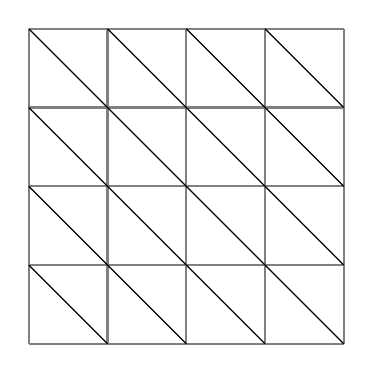
\begin{tikzpicture}
      \draw[step=1cm,gray,thick]
      (0,0) grid (4,4);

      \foreach \x in {0,...,3}{
        \draw (\x, 0) -- (0, \x) ;
        \draw (\x, 4) -- (4, \x) ;
      }

    \end{tikzpicture}
    \caption{Tri-Structured Mesh}
    \label{fig:struct}
  \end{minipage}
  \begin{minipage}{.5\textwidth}
    \centering
    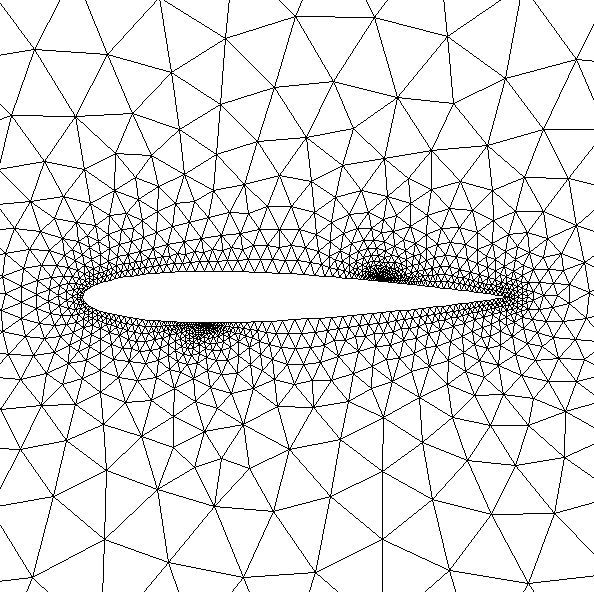
\includegraphics[width=.55\textwidth]{umesh}
    \caption{Airfoil Tri-Unstructed Mesh}
    \label{fig:umesh}
  \end{minipage}
\end{figure}
\par
Unstructed Meshes, such as Figure \ref{fig:umesh}, use connectivity information to specify the mesh topology. The position of elements is highly arbritrary, unlike structured meshes where elements follow a regular pattern (Figure \ref{fig:struct}). A particular simulation might, for example, be approximating the velocity of a fluid in each cell based on the cells around it.

\subsection{Motivations}
The idea for this project was provided by my supervisor, Dr Gihan Mudalige - an Associate Proffesor in the University of Warwick Computer Science Department. It was pulled from the pool of uncompleted features for the OP2 project, and I selected it as it aligned with my interest in High Performance Computing, and similar experience with optimising exisiting codes.
\par
Since OP2 is Open Source and freely available, the implementation I produce will become part of the library, allowing future contributors to build on my work. The project also allows me the opportunity to operate on a large codebase, where most university work is done largely within the confines of one's own code.

% !TEX root =  ../report.tex
% !TeX spellcheck = en-GB

\section{Research}
\label{s:research}
\vspace{-2em}
\subsection{NVidia CUDA Programming Model}
Since this project will require the automatic generation of GPU code source files from sequential code, it is important to introduce the NVidia hardware, and the C Application Programming Interface (API) which will be utilised. NVidia's Compute Unified Device Architecture (CUDA) is used to program their GPUs, which is a proprietary language. Relevant information for this project from the \textit{NVidia CUDA C Programming Guide} \cite{guide} has been summarised below, and it will continue to be used for reference throughout this report.

\subsubsection{Hardware}
The GPU is a computer component that exists alongside the CPU, and communicates on the Peripheral Component Interconnect express (PCIe) bus. The CPU is able to pass workloads over to the GPU for it to execute, particularly compute-heavy workloads which would bottleneck the CPU. As can be seen in Figure \ref{fig:pci}, the GPU has its own onboard memory, and cannot access the computer's RAM directly, so any data that the GPU will process must be copied across the PCIe bus and stored in the GPU's local memory, at the expense of time.

\begin{figure}[h!]
  \centering
  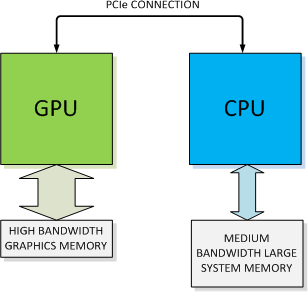
\includegraphics[width=0.37\textwidth]{pci}
  \caption{\label{fig:pci} CPU - GPU communication. Diagram from \cite{nvlink}}
\end{figure}

\par
Figure \ref{fig:arch} contrasts the design of a traditional CPU to that of a GPU, where area of a component corresponds to resources devoted to it. Since the Arithmetic Logic Unit (ALU, coloured green) is responsible for arithmetic operations, and the Cache and DRAM components (coloured orange) will speed up memory operations, it should be clear why the GPU is ideal for compute-heavy workloads, where the ratio of arithmetic operations to memory operations is high.

\begin{figure}[h]
  \centering
  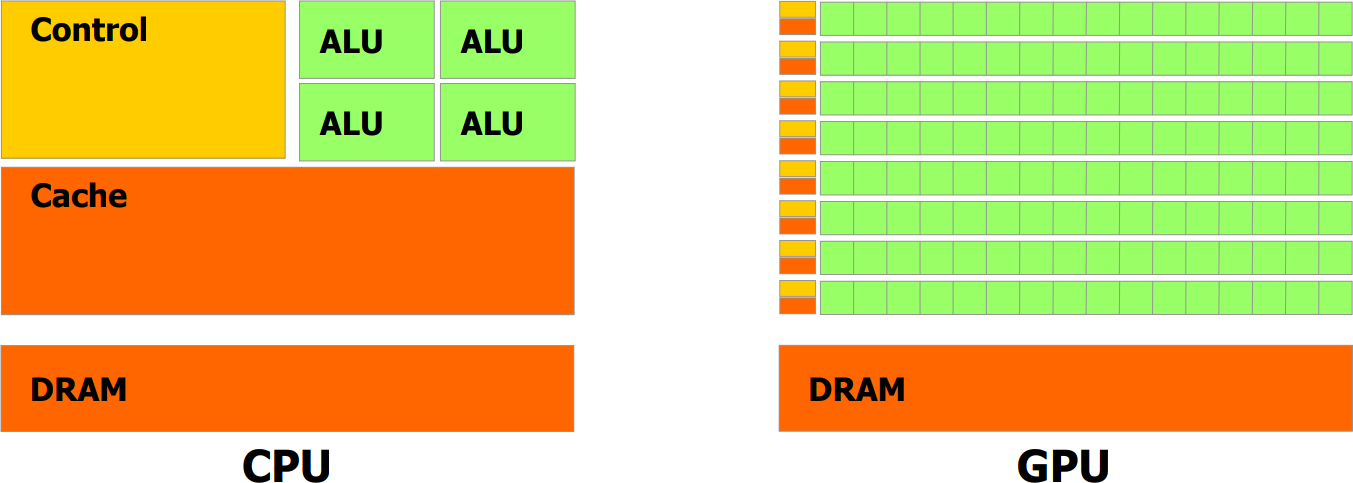
\includegraphics[width=\textwidth]{Architecture}
  \caption{\label{fig:arch} Architecture Comparison. Diagram from \cite[p3]{guide}}
\end{figure}

\par
This structure allows GPUs to excel at performing parallel tasks requiring the same operations to be performed on large sets of data, and therefore well suited to the needs of OP2, where a particular function often need to be repeatedly applied to all edges, cells, or nodes in a given mesh.

\subsubsection{GPU Parallelism}
Workloads executed on a GPU are divided among a Grid of Blocks, where each Block contains a number of Threads, all executing simultaneously in parallel. To allow for easier mapping from the problem space to a Thread Identifier, the Block ID and Thread Identifiers within each block can be 1D, 2D or 3D \cite[p9]{guide}. Figure \ref{fig:threadgrid} shows an example where 2D identifiers are used.

\begin{figure}[h!]
  \centering
  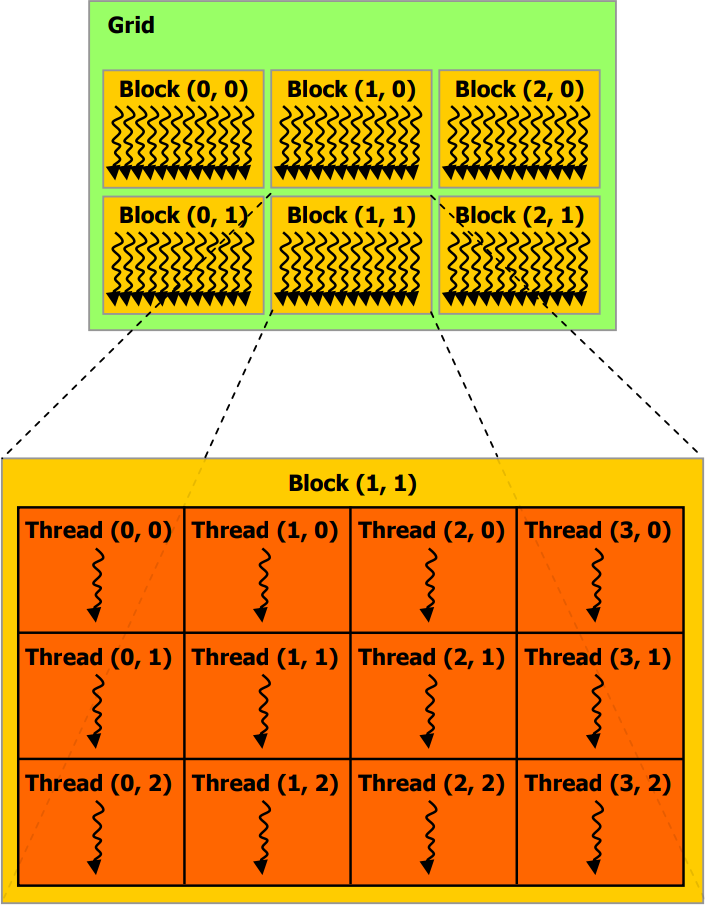
\includegraphics[width=0.6\textwidth]{threadgrid}
  \caption{\label{fig:threadgrid} 2D grid of Blocks and Threads. Diagram from \cite[p9]{guide}}
\end{figure}

\subsubsection{Programming Interface}
The CUDA C API provides two function type quantifiers that will need to be used in the generated code:
\begin{itemize}
\vspace{-.5cm}
\setlength{\itemsep}{0pt}%
\setlength{\parskip}{0pt}%
\item{\verb|__device__|}
\item{\verb|__global__|}
\vspace{-.5cm}
\end{itemize}
Both indicate that the function should be compiled to \textit{PTX}, the CUDA instruction set architecture \cite[p15]{guide}, and executed on an NVidia GPU device. The difference however, is that a function declared \verb|__global__| can be invoked from host (CPU) code, or device (GPU) code; whereas a \verb|__device__| function can only be called from code that is already executing on the device \cite[p81]{guide}.
\par
Global functions therefore act as a sort of entry point into device code. They are called using additional ``execution configuration" syntax \cite[p7]{guide}, added as a C language extension by NVidia, which allows the user to specify special parameters for the required number of blocks, and threads per block:
\codeline{function<<< num_blocks, threads_per_block >>>( [arguments...] )}{}
\noindent Where the data type of \verb|num_blocks| and \verb|threads_per_block| can be a normal, C language \verb|int| type (1D), or use a CUDA type \verb|dim3| \cite[p9]{guide} to specify up to 3 dimensions. Any value left unspecified is initialised as 1 \cite[p87]{guide}. The function body will then be executed $\verb|num_blocks| \times \verb|threads_per_block|$ times, with all threads beginning at the same time. The number of threads has an upper limit depending on the hardware, for example the Kepler Architecture can support 2048 total threads per multiprocessor \cite{kepler}, for example 8 blocks of 16 $\times$ 16 threads (2 dimensions of thread IDs).
\par
Inside the function body built in variables \verb|threadIdx.x|, \verb|blockIdx.x|, and \verb|blockDim.x| can be used to determine the work which a certain thread should carry out, usually by calculating an array index from their values. Appendix \ref{app:cudaEx} is a CUDA program written during research to build familiarity with writing CUDA code, which utilises these constructs and ideas.
\par
In the next section, the OP2 Framework and its existing code generation will be discussed. It can produce optimised code executable on a GPU from unoptimised sequential code, and parts of this code generator will aid in development of the new code generation script being produced for this report, with the Just-In-Time Compilation functionality as an addition.

\subsection{OP2}

\subsubsection{Existing Work}

This project is focussed on a contribution made to the OP2 open source library. There is a large quantity of literature available on the OP2 website \cite{op-dsl}, but the following section aims to provide enough understanding for someone unfamiliar with OP2 to follow the rest of this report.
\par
OP2 is an "active library" framework \cite{op2main}, which takes a single application code written using the OP2 Application Programming Interface (API), embedded in either C or Fortran and uses source-to-source translation to produce multiple different source codes, each targeting a different optimised parallel implementation. The generated source code is then compiled, and linked against the OP2 library files to produce an executable for the original application which will run on the desired platform. It is the extra step of code generation that makes OP2 an "active" library, compared to conventional software libraries.
\par
Since this project is focused on the GPU back-end, the journal article \textit{Designing OP2 for GPU architectures} \cite{gpudesign} is necessary background material, as it covers a lot of important details from the implementation of the existing GPU framework.

\tinytitle{Designing OP2 for GPU architectures}
This article, originally published in the Journal of Parallel and Distributed Computing in 2013, describes the key design features of the current OP2 library for generating efficient code targeting GPUs based on NVidia’s \textit{Fermi} architecture. It is worth noting that \textit{Fermi} is no longer the latest architecture, and the code generation process has been modified since publication, however the article still provides useful information.
\par
One of the key points made in the paper is on the managing of data dependencies (p1454), where an operation relies on another being complete before it can begin, otherwise the result may be incorrect. Solutions include: an owner of node data which performs the computation; colouring of edges such that no two edges of the same colour update the same node; and atomic operations which perform a read-modify-write operation as a single, uninterruptible action on a 32-bit or 64-bit word residing in global or shared memory \cite[p96]{guide}. This means that a thread cannot alter the value in memory between the read and write operations of another thread, which could cause a data dependency to be violated, as all three operations are performed as a single atomic action, and therefore they cannot overlap. \\In the implementation for this project, atomic operations were selected as the best solution for this issue.
\par
The paper also introduces the consideration of data layout in memory. Figure \ref{fig:SoA_v_AoS} demonstrates the different layouts possible when there are multiple components for each element, in this case 4 elements with 4 components each. While using Array-of-Structs is the default layout, and the easier to implement, the paper concludes that transforming application code to utilise the Struct-of-Arrays layout is effective for reducing the total amount data transferred to and from GPU global memory, in some cases by over 50\%.


\begin{figure}[h]
  \centering
  \subfloat[Array-of-Structs (AoS) layout]
  {
    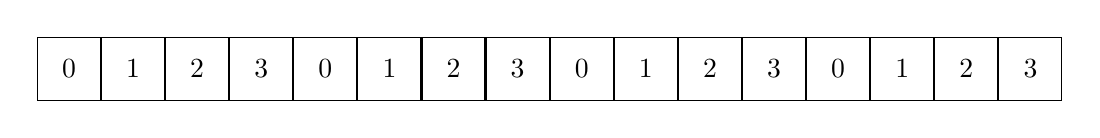
\begin{tikzpicture}[cell/.style={rectangle,draw=black}, ampersand replacement=\&, space/.style={minimum height=1.5em,matrix of nodes,row sep=-\pgflinewidth,column sep=-\pgflinewidth,column 1/.style={font=\ttfamily}},text depth=0.5ex,text height=2ex,nodes in empty cells]

    \matrix (A) [matrix of nodes, nodes={draw, minimum size=8mm}]{
        0 \& 1 \& 2 \& 3 \& 0 \& 1 \& 2 \& 3 \& 0 \& 1 \& 2 \& 3 \& 0 \& 1 \& 2 \& 3\\};
    \end{tikzpicture}
  }

  \quad

  \subfloat[Struct-of-Arrays (SoA) layout]
  {
    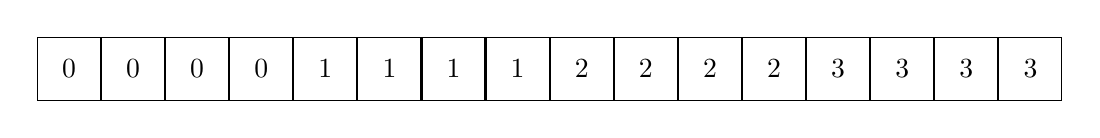
\begin{tikzpicture}[cell/.style={rectangle,draw=black}, ampersand replacement=\&, space/.style={minimum height=1.5em,matrix of nodes,row sep=-\pgflinewidth,column sep=-\pgflinewidth,column 1/.style={font=\ttfamily}},text depth=0.5ex,text height=2ex,nodes in empty cells]

    \matrix (A) [matrix of nodes, nodes={draw, minimum size=8mm}]{
      0 \& 0 \& 0 \& 0 \& 1 \& 1 \& 1 \& 1 \& 2 \& 2 \& 2 \& 2 \& 3 \& 3 \& 3 \& 3\\};
    \end{tikzpicture}
  }
  \caption{\label{fig:SoA_v_AoS} Data layouts. Diagram reproduced from \cite{gpudesign}}
\end{figure}

\noindent The SoA layout is enabled by setting the value of an environment variable:\\ \verb|OP_AUTO_SOA=1|
The environment must be set prior to code generation \cite[p13]{manual}, as it modifies the output of the code generation stage. In the Implementation section (Section \ref{s:impl}) the differences in generated code when this is enabled will be explained in greater detail.
\par
The existing solution is able to generate optimised CUDA code for a parallel loop where the resulting code can map set elements to a GPU thread by which it will be processed, therefore operating on many set elements at once in parallel. It is important to note that the existing implementation for CUDA code generation produces a solution that is compiled entirely ahead of time, i.e.\ prior to the inputs being known, and therefore is not able to make optimisations based on the mesh input. This project aims to bridge this gap, and determine if there is benefit to be gained from such optimisations.
\par
Since OP2 enforces that the order in which the function is applied to the members of the set must not affect the final result \cite[p4]{manual}, the consideration for not violating data dependencies between iterations is removed in the generated code, and therefore loop iterations can be scheduled in any order, based on best performance.

\subsubsection{OP2 Applications}
There are a number of industrial applications that have been implemented using the OP2 active library framework, which would immediately benefit from further optimisation of the generated code, including: \textit{airfoil} \cite{airfoil} - a non-linear 2D inviscid \textit{airfoil} code; \textit{Hydra} \cite{hydra} - Rolls Royce’s turbo-machinery simulator; and \textit{Volna} \cite{volna} - a finite-volume nonlinear shallow-water equation solver used to simulate tsunamis.
\par
They make use of the abstraction provided by the OP2 API to allow scientists and engineers to focus on the description of the problem, and separates the consideration for parallelism, data-movements, and performance into the OP2 library and code generation.
\par
A further benefit is that such applications can be ported onto a new generation of hardware, which could be developed in the future. Only the OP2 back-end library would need to be modified to provide support for the new hardware, instead of every application individually. This portability can save both time and money in development of HPC applications if multiple different hardware platforms are desired to be used.
\par
Later in this report we will see \textit{airfoil} used for benchmarking runtime, to determine whether the new optimisation presented in the report is likely to provide benefit to other OP2 applications.

\subsubsection{OP2 Results}
The optimisation of the Hydra turbo-machinery simulator was presented in a 2016 paper titled \textit{Acceleration of a Full-scale Industrial CFD Application with OP2} \cite{hydrapaper}. This paper compares the newer OP2 framework with its predecessor OPS \cite{ops}, as well as benchmarking the application against OP2 code generated utilising OpenMP \cite{OpenMP} and MPI \cite{MPI} for thread and process level parallelism respectively. Initially, OP2's GPU code generation was outperformed by both OPS generating MPI, and most of the OP2 MPI implementations - completing 45\% slower than the best CPU performance (2 CPUs, 24 MPI processes).
\par However, after some parameters had been tweaked including modifying the block sizes and enabling the Struct-Of-Arrays data layout, a single K20 GPU was able to achieve nearly $1.8\times$ speedup over the original OPlus version, and close to $1.5\times$ over the MPI version of Hydra with OP2. It is worth noting that these MPI implementations are already optimised parallel versions, not sequential implementations, so a speedup of 150\% is a very significant result.
\clearpage

\subsection{Just-In-Time Compilation}
\label{ss:rw_JIT}

The term ``Just-In-Time Compilation" is most commonly associated with the Java programming language, and particularly the Java Run-time Environment (JRE), as ``JIT" Compilation is an integral part of the design and usage of the Java Virtual Machine (JVM).

\par The Java compiler (\verb|javac|) compiles code into platform independent "bytecode" \cite{javac}, then at run-time this bytecode can be interpreted, or compiled a second time by the JVM into native code, and optimised specifically for the machine it is running on. It can also take the program's inputs into account, since they will be known and fixed at run-time.
\par
This re-compilation from bytecode to native code is only done for ``hot" sections which are dominating the runtime \cite{javac}, while the rest continues to be interpreted, as it is not worth the time cost to recompile. Chapter 4 of \textit{Java Performance: The Definitive Guide} \cite{javaPerf} contains further detail on the JIT compiler and its impact on the performance of Java.
\par
The core idea of recompiling code at run-time to obtain performance is the inspiration for the new optimisation investigated in this report, and the origin of its name. However, the Java approach does not exactly map onto OP2. In the existing framework, there is no possibility of intermediate code, and no Virtual Machine in which the binary will execute that can profile the running code and react to ``hot" sections. Instead, an alternative source file at the same ``level" above native code is created (see Figure \ref{fig:jit_compare}). This new source code that has been translated will be able to utilise assertions made using the input data, and so is compiled and used in place of the equivalent but unoptimised functions compiled ahead of time. The design of the JIT compilation system for OP2 will be covered in greater detail in Section \ref{s:spec}.

\begin{figure}[h!]
  \vspace{2em}
  \makebox[\textwidth][c]{
  \resizebox{1.1\textwidth}{!}{
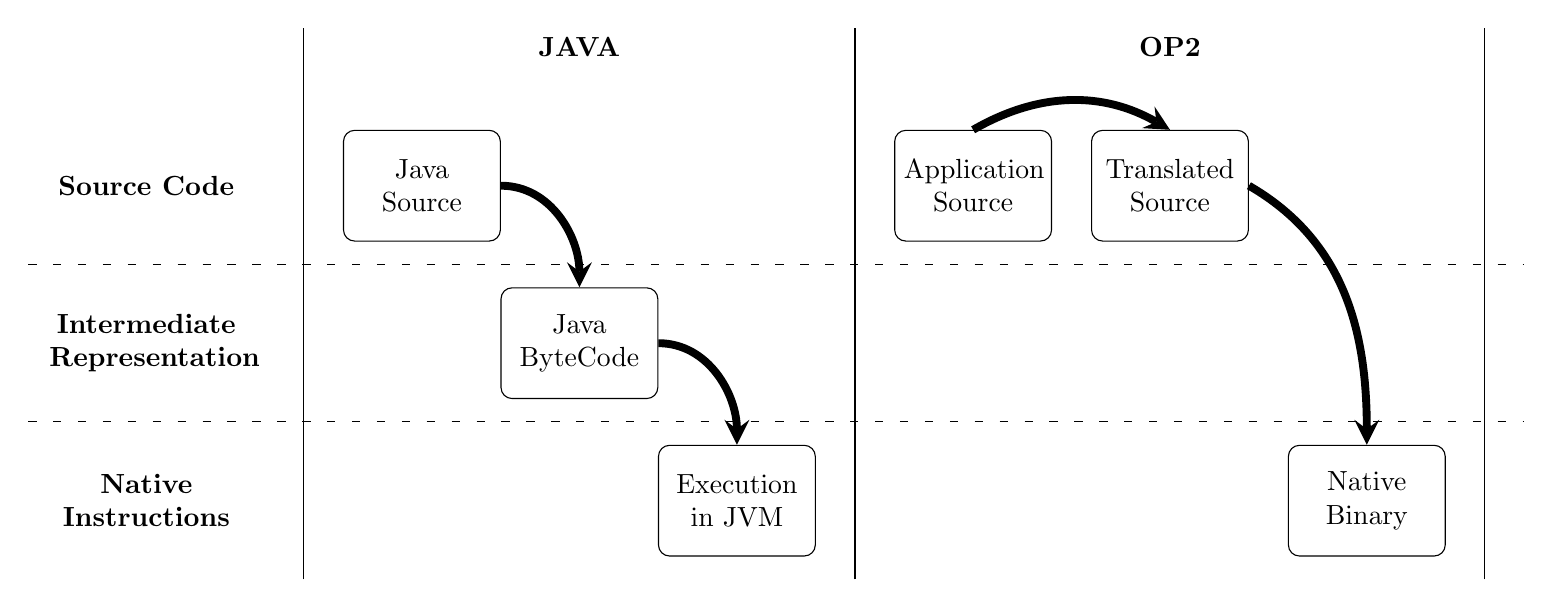
\begin{tikzpicture}

    \tikzstyle{arr} = [->, >=stealth, line width=1mm];
    \tikzstyle{rowtitle} = [text width=7em, text centered, font=\bfseries];

    %\draw [help lines] (0,0) grid (10,6);

    \node [rowtitle] at (0,4) (source) {Source Code};
    \node [rowtitle] at (0,2) (inter) {Intermediate Representation};
    \node [rowtitle] at (0,0) (native) {Native Instructions};

    \draw [loosely dashed] (-1.5,1) -- (17.5,1);
    \draw [loosely dashed] (-1.5,3) -- (17.5,3);

    \draw (2,-1) -- (2,6);
    \draw (9,-1) -- (9,6);
    \draw (17,-1) -- (17,6);

    \node [anchor=north] at (5.5,6) (JAVA) {\textbf{JAVA}};

    \node [wblock] at (3.5,4) (jsource) {Java Source};
    \node [wblock] at (5.5,2) (jbyte) {Java ByteCode};
    \node [wblock] at (7.5,0) (jsvm) {Execution in JVM};

     \node [anchor=north] at (13,6) (OP2) {\textbf{OP2}};
    %
     \node [wblock] at (10.5,4) (appsource) {Application Source};
     \node [wblock] at (13,4) (tsource) {Translated Source};
     \node [wblock] at (15.5,0) (bin) {Native Binary};

     \draw [arr] (appsource.north) to [out=30,in=150] (tsource.north);
     \draw [arr] (tsource.east) to [out=-30,in=90] (bin.north);

     \draw [arr] (jsource.east) to [out=0,in=90] (jbyte.north);
     \draw [arr] (jbyte.east) to [out=0,in=90] (jsvm.north);

\end{tikzpicture}
  }}

  \caption{Comparison of Java and OP2 JIT}
  \label{fig:jit_compare}
\end{figure}

\subsubsection{Related Work}

While Java's JIT compilation gives a good indication that there is real benefit to be gained from using the technique, its implementation does not translate well on to the active library workflow. While researching more similar applications of the concept, the \textit{easy::JIT} library was discovered.\\
\par
\tinytitle{easy::JIT} \textit{easy::JIT} \cite{eJIT} is a library created by Juan Manuel Martinez Caamaño and Serge Guelton of \textit{Quarkslab} \cite{Quarkslab}. It targets C++ code, and utilises \verb|clang| \cite{clang} as the compiler, which is built using the Low Level Virtual Machine (LLVM) framework. It therefore can make use of the LLVM's Intermediate Representation, where other C compilers like \verb|gcc| cannot. \textit{easy::JIT} does also differ from this project however, as it utilises code generation at run-time, and a cache of code to ensure this does not need to be done on every execution. The OP2 implementation discussed in this report will generate all of the code ahead of time, as this is a slow process.
\par
Applications developed for OP2 are not currently limited to only LLVM-based C compilers like \verb|clang|, although a translator using LLVM Intermediate Representation to replace the current Python and MatLab source-to-source translation scripts is currently in development \cite{op2clang}. This would bring it more in line with Java, having an original source, an intermediate representation, and then native code after the second compilation stage.\\
The implementation completed for this report is building on the compiler agnostic OP2 implementation, and therefore will not utilise LLVM .

% !TEX root =  ../report.tex
% !TeX spellcheck = en-GB

\section{Specification}
\label{s:spec}

In order to clearly explain the design of the extension that will be made to the OP2 framework, it is important to first understand the pre-existing work-flow. The following is a high level overview of the components of OP2 that pre-date this project, so that when the new system is described in Section \ref{ss:reqs} it is easier to understand.

\subsection{Pre-Existing System}
\begin{figure}[h!]
\makebox[\textwidth][c]{
 \resizebox{1.1\textwidth}{!}{
  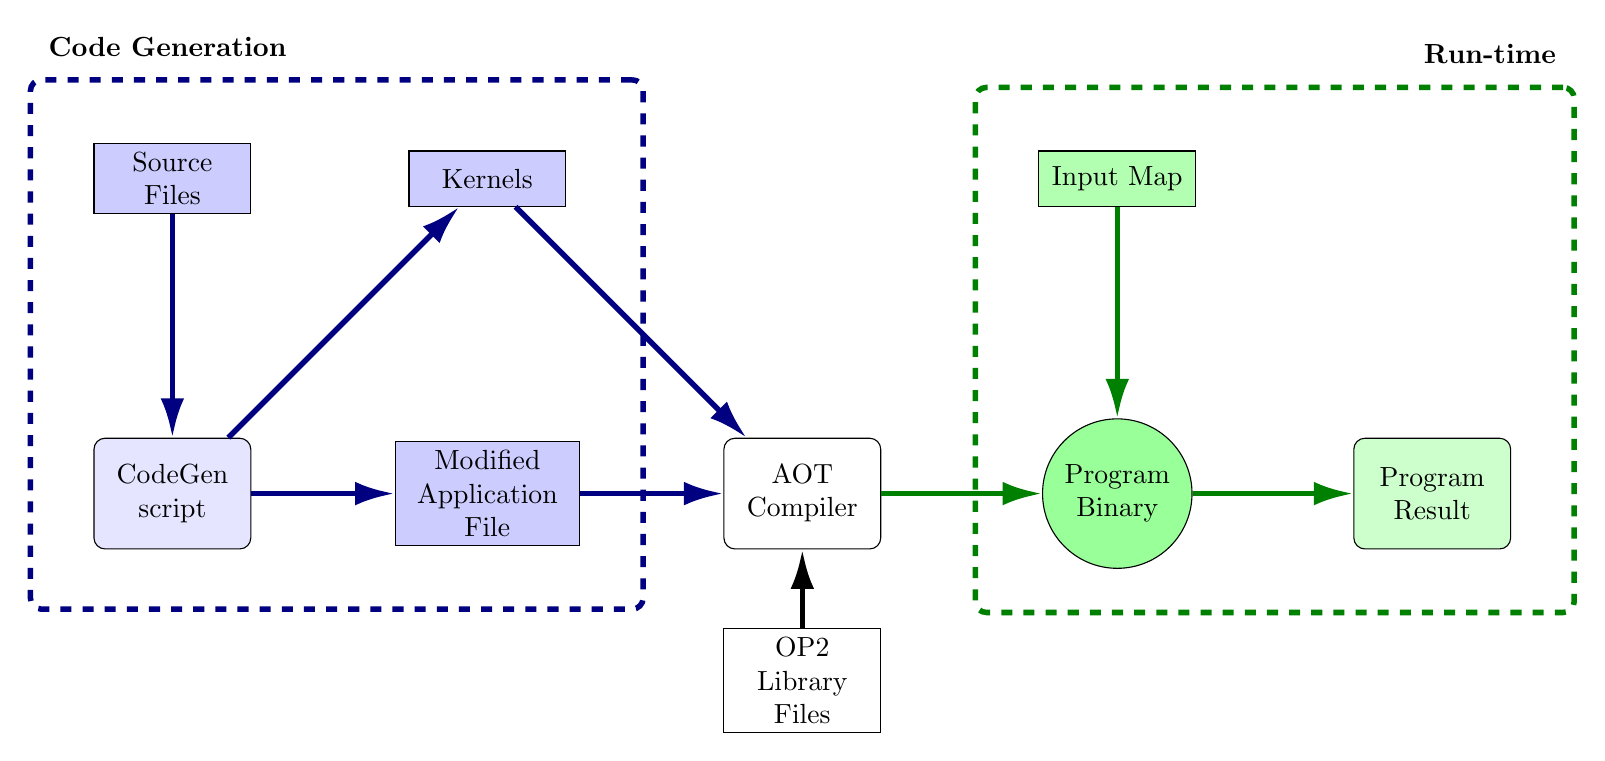
\begin{tikzpicture}[node distance=4cm, auto]
    \node [file] (source) {Source Files};
    \node [block, below of=source] (op2py) {CodeGen script};
    \node [file, right of=op2py, text width=6em] (sourceOp) {Modified Application File};
    \node [file, above of=sourceOp] (Kernels) {Kernels};
    \node [wblock, right of=sourceOp] (aot) {AOT Compiler};
    \node [wfile, below=1cm of aot] (op2lib) {OP2 Library Files};

    \node [rbin, right of=aot] (binary) {Program Binary};
    \node [rfile, above of=binary] (input) {Input Map};
    \node [rblock, right of=binary] (result) {Program Result};

    \tikzset{dotted box1/.style={draw=black!100, dash pattern=on 4pt off 4pt,
      inner sep=8mm, rectangle, rounded corners, line width=2pt}};

    \node (run-time) [dotted box1, fit = (input) (result), color=green!50!black] {};
    \node at (run-time.north east) [above left=2mm] (rtbox) {\textbf{Run-time}};

    \node (code-gen) [dotted box1, fit = (source) (sourceOp), color=blue!50!black] {};
    \node at (code-gen.north west) [above right=2mm] (rtbox) {\textbf{Code Generation}};

    \path [line, color=blue!50!black] (source) -- (op2py);
    \path [line, color=blue!50!black] (op2py) -- (sourceOp);
    \path [line, color=blue!50!black] (op2py) -- (Kernels);
    \path [line, color=blue!50!black] (sourceOp) -- (aot);
    \path [line, color=blue!50!black] (Kernels) -- (aot);
    \path [line, color=black] (op2lib) -- (aot);
    \path [line, color=green!50!black] (aot) -- (binary);
    \path [line, color=green!50!black] (input) -- (binary);
    \path [line, color=green!50!black] (binary) -- (result);

  \end{tikzpicture}
  }}
  \caption{Pre-existing OP2 System Diagram}
  \label{fig:aot_sys}
\end{figure}

\noindent The pre-existing OP2 workflow is shown in Figure \ref{fig:aot_sys}. The diagram starts in the top left with the Code Generation stage, beginning at the system's input: a set of Source Files. The set of Source Files cannot be empty, and must contain a Master Application file. The Master Application file is a normal C program, which makes OP2 API calls to define of sets, maps, and constants, as well as for initialising and cleaning up the OP2 execution with \verb|op_init()| and \verb|op_exit()|. It describes the application structure, and when parallel loops should be executed.
\par
The input Source Files can optionally contain additional C source and header files, included in the normal way with \verb|#include| statements, to assist with the organisation of a complex application with a large code-base. An example usage of these files would be a header file for each parallel loop, containing the function to be executed as the loop body.
\par
These Source Files are parsed by the code generation Python script, from which the output is a modified version of the master application file, and a kernel file for each parallel loop. The output files are compiled, and linked against the OP2 library files for the GPU platform to produce an executable Program Binary. The expectation is that this binary will run without error on the target hardware, taking a map as an input to produce the result desired by the application programmer.
\par
The pre-existing system is able to generate optimised code for GPUs from the high level application code, and apply optimisations ahead of time. It is not, however, able to optimise based on the inputs at all, as they are only known at run-time, after the compiler has completed and the binary is being executed. This is where the implementation for this project comes in: to provide the ability to use the input data when optimising.

\subsubsection{op2.py}
\label{ss:impl_op2}
The code generation is done using Python scripts, with the main script being \verb|op2.py|, which parses the input files to gather data, and provides this data to a number of other scripts. Each of these other scripts performs the code generation for a specific hardware platform. \verb|op2.py| uses the Python Regular Expressions (RegEx) library: \verb|re| \cite{re} to identify OP2 API calls in the Application File, and ensures certain conditions are met - for example that \verb|op_init| and \verb|op_exit| are both called at least once to initialise and clean up the OP2 execution environment.
\par
Information is also gathered during the parse about each parallel loop, including the number of the parameters and their types, and the details of the indirect data set if the loop is indirect. This stage includes some error checking, by ensuring types and dimensions are consistent throughout the application.
\par
Once the Application has been analysed, \verb|op2.py| produces a modified copy of the Application File, named \verb|[application]_op.cpp|, which is largely the same as the file provided by the application programmer, but with the addition of \verb|extern| declarations for the function each parallel loop will call: \verb|op_par_loop_[name]|. Defining a function \verb|extern| means it has external linkage \cite{linkage}, and therefore the definition of the function may be found during the linking stage of compilation, not in the current pass.
\par
The generator scripts for each platform will receive the list of loop details gathered using RegEx as its parameters, then will generate a definition of every parallel loop's execute function in the form of Kernel files. At compile-time the definitions given in these Kernel files will be linked to the extern declaration in the Modified Application File by the linker.
\par
The requirements for the code generation script that will be created as part of this project, that will produce kernels containing CUDA code with JIT compilation, will be discussed in the following section.

\subsection{New System Requirements}
\label{ss:reqs}

Implementing the new system will require work in two main areas: a new Python code generation script, and some modifications to the OP2 library itself. The OP2 Library is currently implemented in both C and Fortran, but only the C library will be modified, due to developer familiarity with the C language. OP2 does also include code generation using MatLab, however the Python script is preferable for new developments, since Python is now ubiquitous, and provides very convenient string manipulation capabilities. The following are the necessary requirements to consider this project a success.

\subsubsection{Python Script}
The new code generation script will be named \verb|op2_gen_cuda_jit.py|, and will need to perform a somewhat similar source-to-source translation process to pre-existing CUDA script for Ahead-Of-Time (AOT) compiled code. The extension required is the ability to also generate a second, altered code-base that will be compiled at run-time, as well as the original code that is compiled prior to running the executable.
\par
All code generated by the new code generation script must form valid C files, and compile using a the Intel C compiler \cite{icc} without errors. Since the project will involve generation of NVidia CUDA as well, the generated CUDA code must also be valid, and compile with the NVidia C Compiler (\verb|nvcc|) from the NVidia CUDA Toolkit \cite{nvcc,toolkit} without errors.
\par
When the resulting executable which has been compiled from the generated code is executed, it will need to invoke a re-compilation stage while it is running, and execute code that has been compiled during its runtime as part of its execution. It must produce an output within some tolerance of the expected result, obtained from executing the parallel loop iterations sequentially in an arbitrary order. The order is not significant, as OP2 enforces a restriction that the order in which elements are processed must not affect the final result, within the limits of finite-precision floating-point arithmetic \cite[p3]{op2main}.
\par
Lastly, the above requirements must be met for both Array-of-Structs and Struct\\-of-Arrays data layouts, especially when automatic SoA conversion is enabled, as this alters the generated code.

\subsubsection{Run-time Assertions}
The application's input will be a large number of data points forming an unstructured mesh which it will operate over. The optimisation that will be made for this project is "Constant Definition", built on the assertion that values declared as OP2 constants are certainly not going to change during the course of execution. To apply this optimisation, constant values provided as part of the input must be turned into \verb|#define| directives for the C pre-processor in the recompiled code. This will result in all references to the variable's identifier in the code being transformed so they are seen as a literal value rather than a memory read by the compiler.
\par
An example of how this is normally used can be seen in the CUDA example program from before (Appendix \ref{app:cudaEx}), where the size of the arrays to be added together is defined as \verb|N|, and everywhere \verb|N| appears in the code the literal value \verb|32| will be substituted before compilation.
\par
As a result of the need to store constant values in memory being removed, retrieval time from memory when a constant value is required has been eliminated. The literal value is immediately available. Other possible optimisations will be discussed in Section \ref{ss:fw} (Future Work).
\par
The overall goal of this project is to investigate whether this technique does provide any performance benefit, however any performance increase that incurs unacceptable deviation from the expected result is not a useful benefit. Therefore, the addition of defined constants should not reduce the accuracy of the result outside tolerance. It is not expected that it will.


\subsubsection{OP2 Library}
Outside the translation script, some OP2 API functions may need to be implemented differently in the OP2 library files, as the functions may require additional information to be stored and retrieved at runtime. It is a requirement that the OP2 API itself is not altered in any way by modifications to the library, so that all existing programs currently using the API will be able to seamlessly update to using the modified version.

\subsection{Testing \& Benchmarking}
Once the code generation stage has been completed, and the Python Script is able to generate valid C and CUDA code that can be compiled without error for an example OP2 Application, the resulting binary needs to be tested to ensure the result is correct, and its runtime needs to be benchmarked to determine if there is performance gain.
\par
The runtime will be compared against the same application generated for graphics cards without JIT compilation, to see if there is any benefit. Benchmarking results will include the time taken to recompile at runtime for the JIT compiled version, and the time taken to copy constant values to device memory for the AOT compiled version.


\clearpage
\subsection{New System Model}

\begin{figure}[h!]
\makebox[\textwidth][c]{
\resizebox{1.1\textwidth}{!}{
  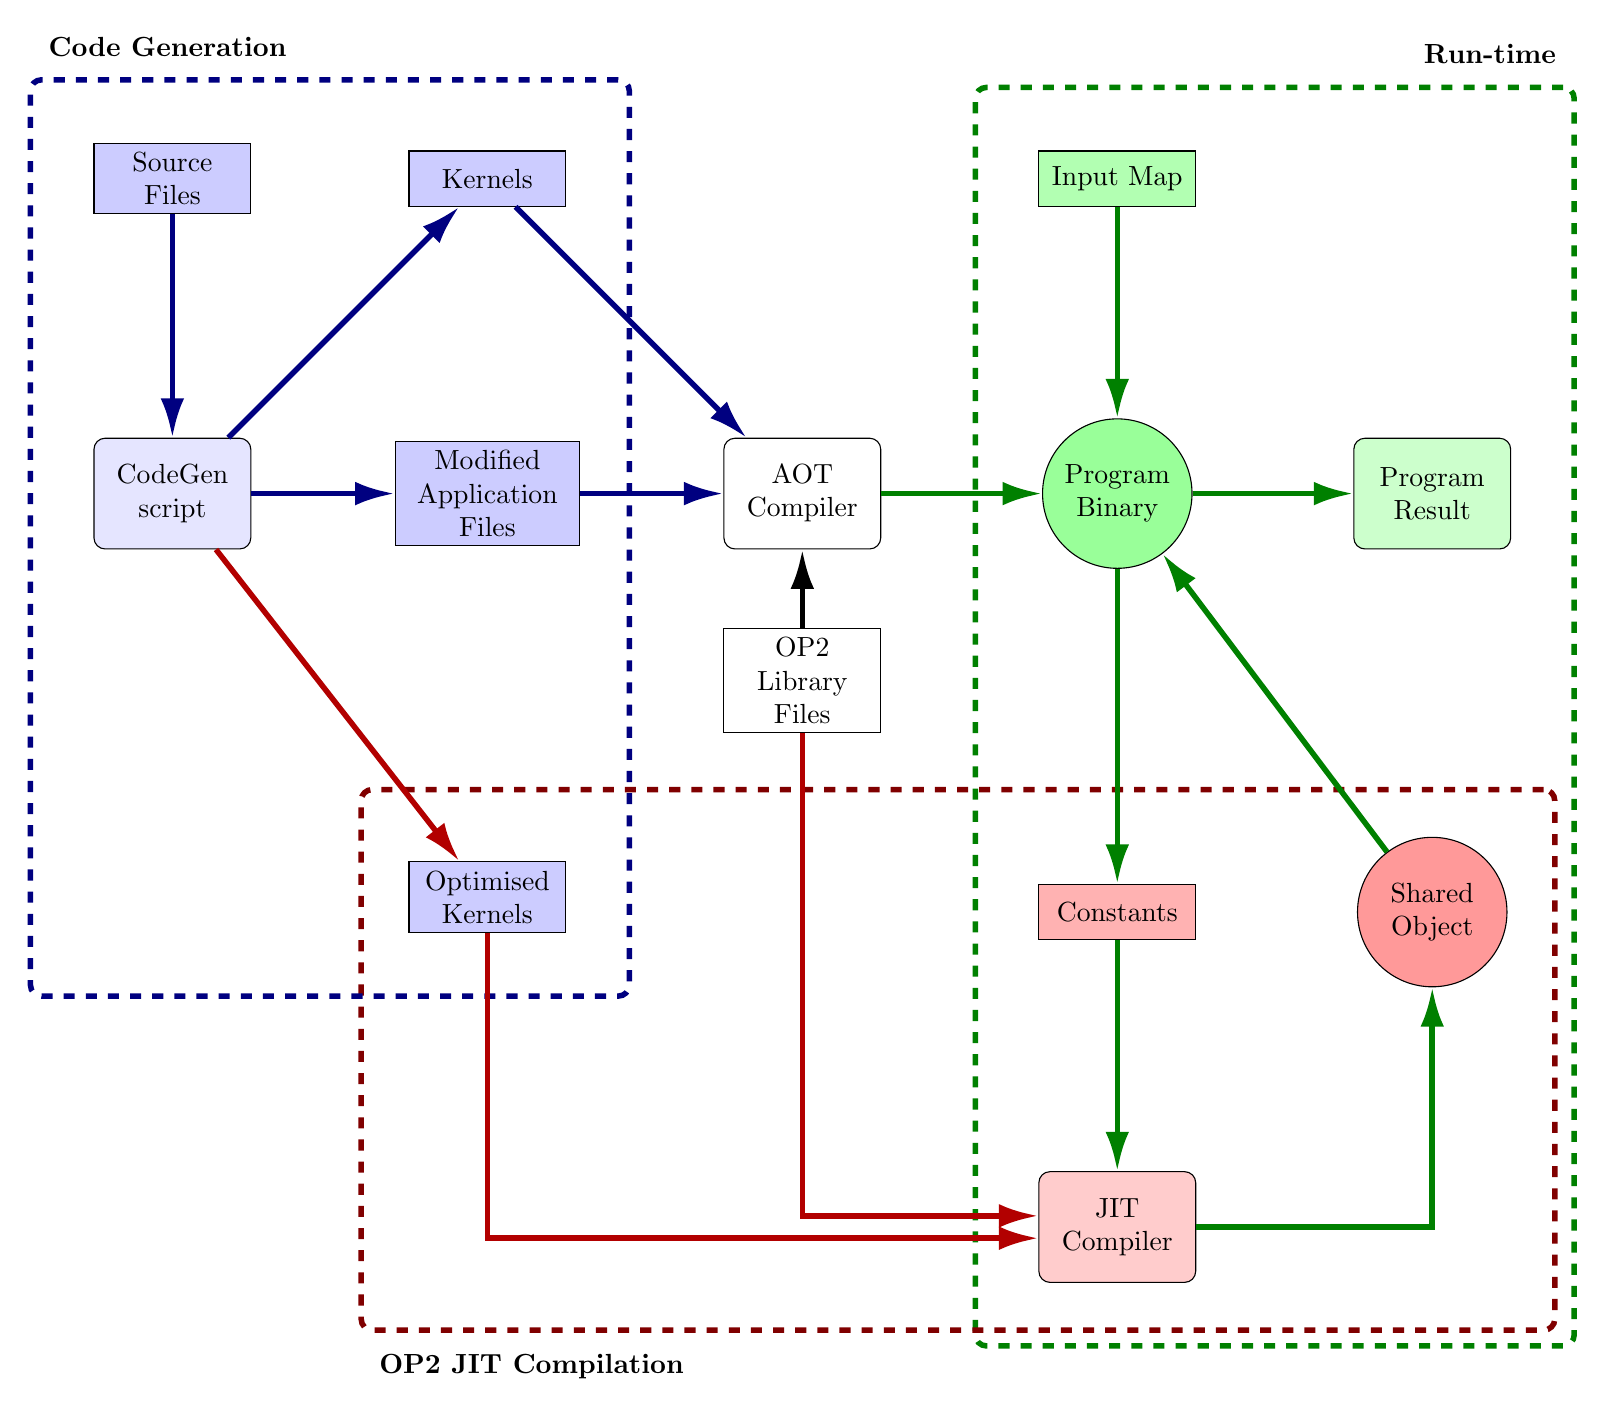
\begin{tikzpicture}[node distance=4cm, auto]
    \node [file] (source) {Source Files};
    \node [block, below of=source] (op2py) {CodeGen script};
    \node [file, right of=op2py, text width=6em] (sourceOp) {Modified Application Files};
    \node [file, above of=sourceOp] (Kernels) {Kernels};
    \node [wblock, right of=sourceOp] (aot) {AOT Compiler};
    \node [wfile, below=1cm of aot] (op2lib) {OP2 Library Files};

    \node [rbin, right of=aot] (binary) {Program Binary};
    \node [rfile, above of=binary] (input) {Input Map};
    \node [rblock, right of=binary] (result) {Program Result};

    \node [file, below=4cm of sourceOp] (recKernels) {Optimised Kernels};
    \node [jfile, below=4cm of binary] (consts) {Constants};
    \node [jblock, below of=consts] (jit) {JIT Compiler};
    \node [jbin, right of= consts] (so) {Shared Object};

    \tikzset{dotted box1/.style={draw=black!100, dash pattern=on 4pt off 4pt,
      inner sep=8mm, rectangle, rounded corners, line width=2pt}};
    \tikzset{dotted box2/.style={draw=black!100, dash pattern=on 4pt off 4pt,
      inner sep=6mm, rectangle, rounded corners, line width=2pt}};

    \node (run-time) [dotted box1, fit = (input) (jit) (result), color=green!50!black] {};
    \node (jitbox) [dotted box2, fit = (recKernels) (so) (jit), color=red!50!black] {};

    \node at (run-time.north east) [above left=2mm] (rtbox) {\textbf{Run-time}};
    \node at (jitbox.south west) [below right=2mm] (corner) {\textbf{OP2 JIT Compilation}};

    \node (code-gen) [dotted box1, fit = (source) (recKernels), color=blue!50!black] {};
    \node at (code-gen.north west) [above right=2mm] (rtbox) {\textbf{Code Generation}};

    \path [line, color=blue!50!black] (source) -- (op2py);
    \path [line, color=red!70!black] (op2py) -- (recKernels);
    \path [line, color=blue!50!black] (op2py) -- (sourceOp);
    \path [line, color=blue!50!black] (op2py) -- (Kernels);
    \path [line, color=blue!50!black] (sourceOp) -- (aot);
    \path [line, color=blue!50!black] (Kernels) -- (aot);
    \path [line, color=black] (op2lib) -- (aot);
    \path [line, color=red!70!black] (op2lib) |- ($(jit.west)!0.2!(jit.north west)$);
    \path [line, color=green!50!black] (aot) -- (binary);
    \path [line, color=green!50!black] (input) -- (binary);
    \path [line, color=green!50!black] (binary) -- (consts);
    \path [line, color=red!70!black] (recKernels) |- ($(jit.west)!0.2!(jit.south west)$);
    \path [line, color=green!50!black] (consts) -- (jit);
    \path [line, color=green!50!black] (jit) -| (so);
    \path [line, color=green!50!black] (so) -- (binary);
    \path [line, color=green!50!black] (binary) -- (result);

  \end{tikzpicture}
  }}
  \caption{OP2 System Diagram with JIT Addition}
  \label{fig:jit_sys}
\end{figure}

\noindent Figure \ref{fig:jit_sys} describes the new workflow of the OP2 library, with Just-In-Time compilation (denoted with a dotted red box). As before, code generation takes an input of the application and optional additional files, and generates the Kernels and Modified Application Files. It also generates an additional set of Optimised Kernels, which contain code that will only be compiled inside the green box denoting `run-time', at which point the constants from the Input Map are known to the program. These Kernel files are not seen by the Ahead-Of-Time compiler.
\par
The JIT compilation will take place during the execution of the binary, and will therefore make up part of the program's execution duration. It will need to link the Optimised Kernels against the OP2 Library Files, so it is necessary that they are stored in a location that is also accessible at run-time, not just when the executable is compiled.
\par
The result of JIT compilation will be a Shared Object file, otherwise known as a Dynamically Loaded Library (DLL) file, with a standardised name. The program can then load this Shared Object and utilise its exported functions, which will be the recompiled versions of each parallel loop. As black boxes the two are equivalent (i.e.\ they have the same inputs and outputs), however theoretically the recompiled versions are faster to execute than the original versions.

\tinytitle{Ahead-Of-Time Kernels}

\noindent The Kernels compiled ahead of time could be altered such that their sole purpose is to invoke the compiler at runtime, then pass execution over to the JIT compiled function. It will be beneficial, however, to allow executables with the JIT compilation feature enabled or disabled to be compiled from the same source code.
\par
This requires the Ahead-Of-Time Kernels to retain the ability to execute the loop body without requiring JIT compilation, as well as being able to initiate the runtime compilation of the optimised kernels. Constant values should still be copied to device memory, but only if the re-compiled kernels will not be used, and copying the values is necessary.
\clearpage
\subsection{Library Modifications}
In the OP2 library, the main API function that will need to be modified is:
\codeline{void op_decl_const(int dim, char *type, T *dat, char *name)}{\cite[p9]{manual}}
\noindent This function is used to declare a constant value, its dimension, data type, and identifier.
Previously, this function copied the value to a device symbol, so that when required it could be read from device memory. In the implementation for this project, it will need to maintain a de-duplicated list of identifiers, and persist their values, data types, and dimensions. These parameters will be used when the first parallel loop is invoked to generate a header file, at which point it is known that no more constants can be declared. In the header file, each of the constant values will have a \verb|#define| directive making the value available as a literal value.\par
In the next section, the completed implementation is discussed. The contents of the files generated by the Python code generation script will be examined in more detail, and design decisions that were made will be explained. The Implementation is presented in its finished form, however the development process is covered later, in Section \ref{ss:pm}.

% !TEX root =  ../report.tex
% !TeX spellcheck = en-GB

\section{Implementation}
\label{s:impl}
The new optimisation of adding a compilation stage during runtime, and defining constants from the input, was implemented over the course of approximately 50 hours as part of this project. The following Section describes the completed addition to the OP2 Framework.

The source code for the existing OP2 Library is hosted open source as a GitHub\cite{OP2rep} repository. Instructions for obtaining the version described in the following section, and for getting started with OP2, are provided in Appendix \ref{app:getStart}.
\subsection{Git Repository}
In the Git Repository, the feature branch for this project is named \verb|feature/jit|. It was branched from \verb|feature/lazy-execution| on 13th November 2019, which was last committed to in April 2018, and therefore it lagged behind the \verb|master| branch somewhat. \verb|feature/lazy-execution| needed to be synchronised with the \verb|master| branch before any other changes could be made.
\par
A rebase was selected as the best method of synchronisation. In git terminology, a rebase involves making copies of a branch's commits, and "re-playing" these changes on to the top of another branch \cite{scm-rebase}. In this case, making copies of all commits made to \verb|feature/lazy-execution| and applying them to the latest commit of \verb|master|. The result once any merge conflicts are resolved will be a code-base with all the features of both branches available.
\begin{figure}[t]
  \centering
  \caption{Rebase vs. Merge. Diagram reproduced from \cite{scm-rebase}}
  \label{fig:git_merge}

  \subfloat
  {
    \makebox[\textwidth][c]{
    \resizebox{.45\textwidth}{!}{
    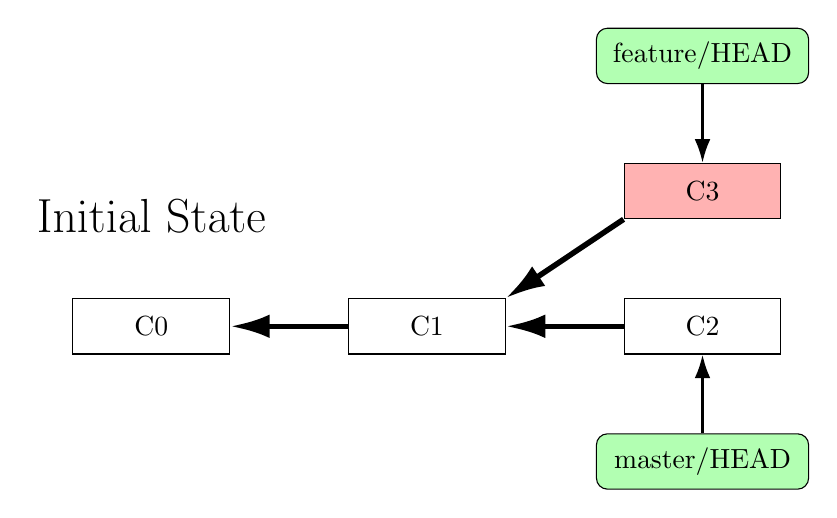
\begin{tikzpicture}[node distance=3.5cm, auto]

      %
      % Initial
      %

      \tikzstyle{label} = [rblock, text width=7em, minimum height=2em, fill=green!30]

      \node [wfile] (C0) {C0};
      \node [wfile, right of=C0] (C1) {C1};
      \node [wfile, right of=C1] (C2) {C2};
      \node [jfile, above=1cm of C2] (C3) {C3};
      \node [label, above=1cm of C3] (fhead) {feature/HEAD};
      \node [label,  below=1cm of C2] (mhead) {master/HEAD};

      \node [above=2em of C0] (initial) {\LARGE Initial State};

      \path [line] (C1) -- (C0);
      \path [line] (C2) -- (C1);
      \path [line] (C3.south west) -- (C1.north east);
      \path [thinline] (fhead) -- (C3);
      \path [thinline] (mhead) -- (C2);

    \end{tikzpicture}
    }}}
    \newline
    \subfloat
    {
      \makebox[\textwidth][c]{
      \resizebox{1.2\textwidth}{!}{
      \begin{tikzpicture}[node distance=3.5cm, auto]

      \tikzstyle{label} = [rblock, text width=7em, minimum height=2em, fill=green!30]

      %
      % Rebase
      %

      \node [wfile, below=6cm of C0] (fC0) {C0};
      \node [wfile, right of=fC0] (fC1) {C1};
      \node [wfile, right of=fC1] (fC2) {C2};
      \node [jfile, above=1cm of fC2, opacity=0.2] (fC3) {C3};
      \node [label, below=1cm of fC2] (fmhead) {master/HEAD};

      \node [above=2em of fC0] (rebase) {\LARGE Rebased Commits};

      \node [jfile, right of=fC2] (fC3prime) {C3'};
      \node [label, above=1cm of fC3prime] (ffhead) {feature/HEAD};

      \path [line] (fC1) -- (fC0);
      \path [line] (fC2) -- (fC1);
      \path [line, opacity=0.2] (fC3.south west) -- (fC1.north east);
      \path [thinline] (ffhead) -- (fC3prime);
      \path [line] (fC3prime) -- (fC2);
      \path [thinline] (fmhead) -- (fC2);

      %
      % Merge
      %

      \node [wfile, right=3cm of fC3prime] (mC0) {C0};
      \node [wfile, right of=mC0] (mC1) {C1};
      \node [wfile, right of=mC1] (mC2) {C2};
      \node [jfile, above=1cm of mC2] (mC3) {C3};
      \node [label, above=1cm of mC3] (mfhead) {feature/HEAD};

      \node [wfile, right of=mC2] (mC4) {C4};
      \node [label, below=1cm of mC4] (mmhead) {master/HEAD};

      \node [above=2em of mC0] (merge) {\LARGE Merged Commits};

      \path [line] (mC1) -- (mC0);
      \path [line] (mC2) -- (mC1);
      \path [line] (mC3.south west) -- (mC1.north east);
      \path [line] (mC4) -- (mC2);
      \path [line] (mC4.north west) -- (mC3.south east);
      \path [thinline] (mfhead) -- (mC3);
      \path [thinline] (mmhead) -- (mC4);


      \end{tikzpicture}
    }}}
\end{figure}
\par
Figure \ref{fig:git_merge} outlines the differences between synchronisation using \verb|rebase|, and the more commonly used \verb|merge|. For this project, rebasing was preferable to merging as a synchronisation action, as the result is a linear branch history, rather than creating a diamond. This is a destructive action, i.e. the git history is re-written, but it allows a future viewer to easily follow the origin of each line of code. Using rebase also avoids modifying the master branch.
\par
Furthermore, in the case of merge conflicts (where a change has been made in both branches, and one needs to be selected) a rebase will halt at the first conflicting commit and allow the conflict to be resolved \cite{rebase-doc}, while synchronising using merge would result in receiving all conflicts in one go, which can make the necessary resolution of the conflicts harder, especially if not familiar with either of the branches, and which change is the newest.
\par
The downside of rebasing is it can be harder to recover from an erroneous rebase, than an erroneous merge. This is due to the fact that merges are not destructive, since they do not re-write history in the same way as a rebase. This will not be an issue here however, since it was unlikely the rebase would need to be undone, and the previous state of both branches remains untouched since a new one is being created.
\par
The \verb|feature/lazy-execution| branch was created for developing a system to execute parallel loops when resulting values are required, rather than when they are called. This functionality will be achieved using an internal library function:
\codeline{void op_enqueue_kernel(op_kernel_descriptor *desc)}{op2/c/src/core/op\_lazy.cpp [71-89]}
\noindent Currently this function executes the queued loop as soon as it is invoked, but there is ongoing work into determining when the result of the loop will be needed, and potentially compressing multiple queued actions into fewer to save time. Lazy execution will not be the focus of this project, however this process for invoking parallel loops will continue to be utilised throughout the work done to enable Just-In-Time Compilation for CUDA, so that future efforts towards lazy execution can be continued on top of the JIT compilation implementation.

\subsection{Code Generation}
\label{ss:codegen}
As described in the Specification before, the majority of the Implementation work can be found in a Python code generation script named \verb|op2_gen_cuda_jit.py|, which is located in the folder: \verb|translator/c/python/jit/| of the OP2 repository.
\par This code generator, which produces source files for CUDA with JIT compilation, is called from another Python script named \verb|op2.py| which was explained in the Section \ref{ss:impl_op2}. \verb|op2.py| can be found in the parent directory: \verb|translator/c/python/|, and its purpose is to handle the generation of the Modified Application File. Since the existing Modified Application File generation is sufficient to meet the requirements of this project, \verb|op2.py| is only slightly changed. The modification made is adding a call to the new code generator described below.

\subsubsection{jit/op2\_gen\_cuda\_jit.py}
The entry point function for the new CUDA JIT code generation script is:
\pyline{op2_gen_cuda_jit(master, date, consts, kernels)}{translator/c/python/jit/op2\_gen\_cuda\_jit.py [102]}
\noindent The arguments passed to it from \verb|op2.py| are:
\begin{center}
\begin{tabular}{>{\bfseries}l l}
master: & The name of the Application file \\[\medskipamount]
date: & The exact date and time of code generation \\[\medskipamount]
consts: & list of constants, with their type, dimension and name \\[\medskipamount]
kernels: & \parbox[t]{.8\textwidth}{list of kernel descriptors, where each element is a map containing many fields describing the kernel.} \\[\medskipamount]
\end{tabular}
\end{center}
\vspace{1em}
\noindent The \verb|kernels| argument serves as the primary input that the output will be most affected by. The output will be two C source code files, referred to as \textbf{kernel files}, for each parallel loop. They will have the following naming scheme:
\begin{itemize}
\vspace{-.5em}
\item{AOT: \verb|cuda/[name]_kernel.cu|}
\vspace{-.5em}
\item{JIT: \verb|cuda/[name]_kernel_rec.cu|}
\end{itemize}

\begin{wrapfigure}[5]{r}{.4\textwidth}
  \vspace{-1cm}
\resizebox{0.4\textwidth}{!}{
  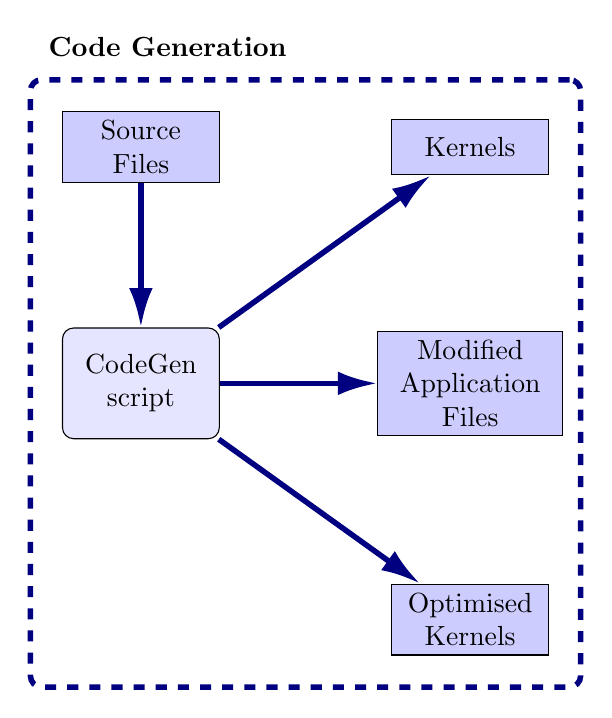
\begin{tikzpicture}[node distance=3cm, auto]
    \node [file] (source) {Source Files};
    \node [block, below of=source] (op2py) {CodeGen script};
    \node [file, right=2cm of op2py, text width=6em] (sourceOp) {Modified Application Files};
    \node [file, above of=sourceOp] (Kernels) {Kernels};

    \node [file, below of=sourceOp] (recKernels) {Optimised Kernels};

    \tikzset{dotted box1/.style={draw=black!100, dash pattern=on 4pt off 4pt,
      inner sep=4mm, rectangle, rounded corners, line width=2pt}};

    \node (code-gen) [dotted box1, fit = (source) (recKernels), color=blue!50!black] {};
    \node at (code-gen.north west) [above right=2mm] (rtbox) {\textbf{Code Generation}};

    \path [line, color=blue!50!black] (source) -- (op2py);
    \path [line, color=blue!50!black] (op2py) -- (recKernels);
    \path [line, color=blue!50!black] (op2py) -- (sourceOp);
    \path [line, color=blue!50!black] (op2py) -- (Kernels);
  \end{tikzpicture}
  }
\end{wrapfigure}
\noindent In the JIT filename ``\verb|_rec|" is short for ``recompiled". These files were referred to as ``Kernels" and ``Optimised Kernels" respectively in the System Model from Section \ref{s:spec}.

\clearpage
A single \textbf{central kernels file} is also generated in the same folder, which is shared between all parallel loops:
\begin{itemize}
\vspace{-.5em}
\item{\verb|cuda/[application]_kernels.cu|}
\end{itemize}
It will contain function definitions required by all loops, or by the Application File; as well as include statements for each of the parallel loops' AOT kernels so they are collated into a single file by the compiler.

\subsubsection{Execution Setup}
The first action performed by the code generation script when it is invoked is to check across all kernels for the Struct-of-Arrays data layout, or if all are using the default Array-of-Structs. If any do use SoA, a flag named \verb|any_soa| becomes a non-zero value, so will evaluate as \verb|True| in a conditional.
\par Then, a folder \verb|cuda/| is created if it does not already exist, and the script will iterate over each kernel, generating both the Ahead-Of-Time (AOT) kernel file, and the Just-In-Time (JIT) kernel file simultaneously.

\subsubsection{Kernel Files}
\label{ss:krnl_files}
As mentioned above, the code generator outputs two C source code files for each parallel loop. The following section explains these kernel files, covering the purpose of each function in the order they are generated, and how they can vary based on the inputs.
\par To avoid ambiguity between code written by the developer, and code that has been generated as part of the output, Python code that is an extract of the implementation will be marked with just a file and line reference, and C code that has been generated as part of the output of the script will be marked \textit{generated by ...} and then a file and line reference.
\par Furthermore, Python code will also always be in a frame filled grey, while generated C code will be in green, blue or red frame - depending on if the code contained in the box is unique to the JIT kernel, the AOT kernel, or is common to both.

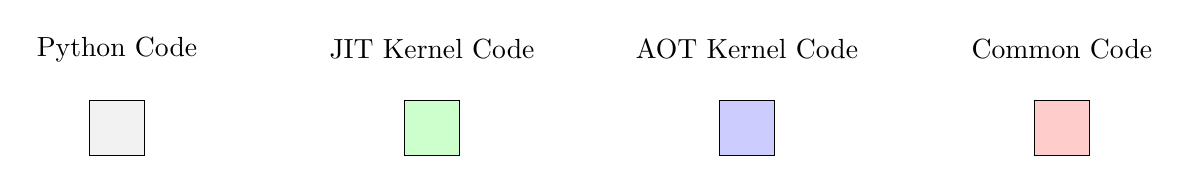
\begin{tikzpicture}
\centering
\node[draw, rectangle, minimum height=2em, minimum width=2em, fill=lightgray!20] at (0,0) (py) {};
\node[text centered] at (0,1) {Python Code};
\node[draw, rectangle, minimum height=2em, minimum width=2em, fill=green!20] at (4,0) (py) {};
\node[text centered] at (4,1) {JIT Kernel Code};
\node[draw, rectangle, minimum height=2em, minimum width=2em, fill=blue!20] at (8,0) (py) {};
\node[text centered] at (8,1) {AOT Kernel Code};
\node[draw, rectangle, minimum height=2em, minimum width=2em, fill=red!20] at (12,0) (py) {};
\node[text centered] at (12,1) {Common Code};


\end{tikzpicture}

\par
Figures \ref{fig:jit_include}-\ref{fig:loop_func} show the progression of the two kernel files for a typical parallel loop during the execution of the code generation script (starting from empty files). They are provided only for the purpose of highlighting the relevant sections of each file. The generated code in the figures is not intended to be a legible size.
\par
It may aid in understanding to follow this section with either the translation script, or a set of generated kernel files to hand, since  full code listings are not included for every section. A summary of the generated functions can be found on page \pageref{impl_summary}.

% May need to move
\clearpage
%
\begin{wrapfigure}[16]{r}{.33\textwidth}
  \centering
  \caption{JIT includes}
  \label{fig:jit_include}
  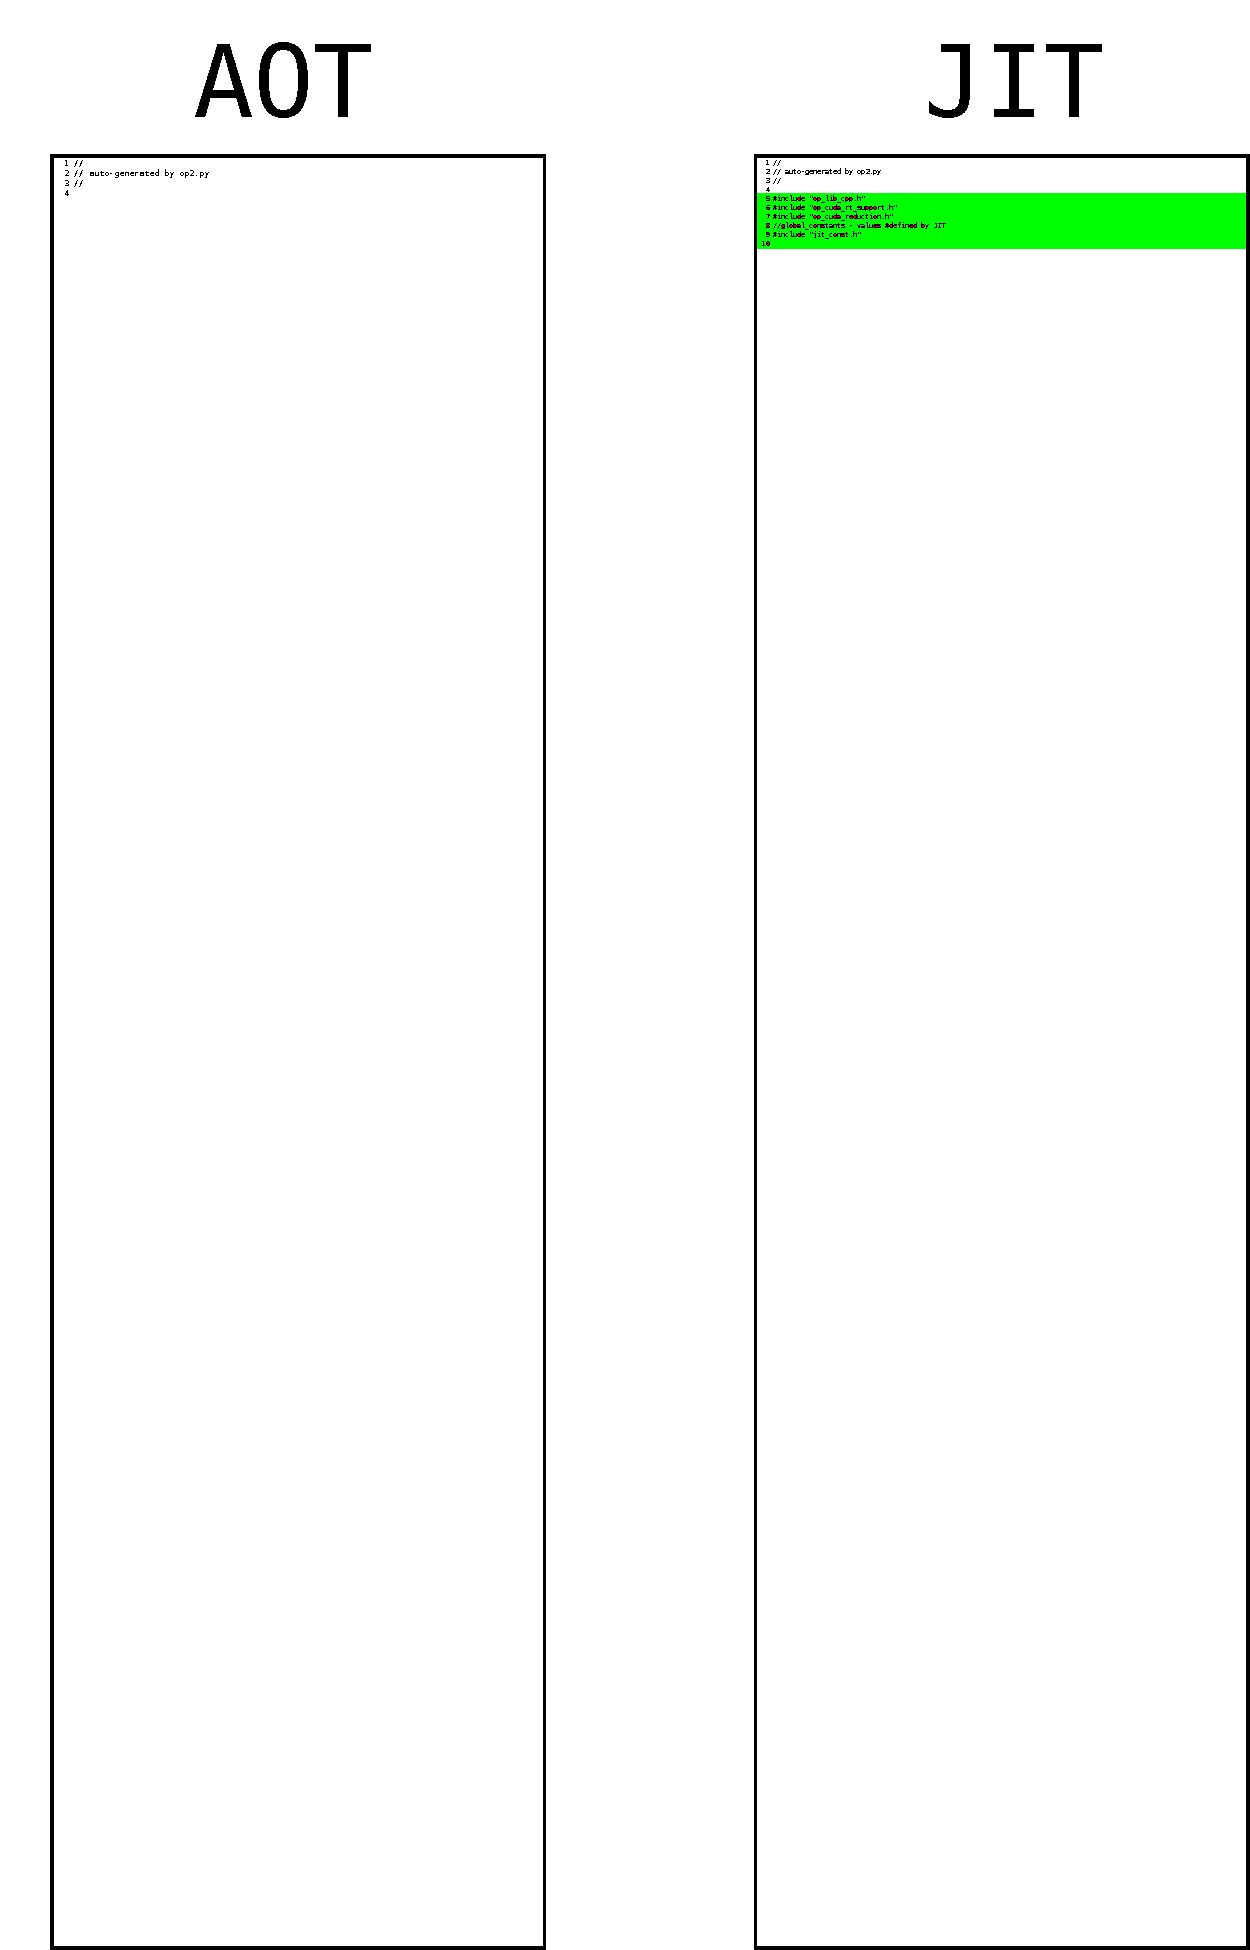
\includegraphics[width=.3\textwidth]{jit_include}
\end{wrapfigure}
\minititle{JIT includes}
The first piece of C code generated by the Python script is simply OP2 library include directives. These are only needed for JIT compiled kernels since they will be processed individually by the compiler, so each requires a reference to the OP2 library files.
\par
They are not needed by AOT kernels, as they will be included by the central kernels file, which will contain these same \verb|#include| statements:
\begin{lstlisting}[backgroundcolor = \color{green!20}, language=C]
 #include `op_lib_cpp.h'
 #include `op_cuda_rt_support.h'
 #include `op_cuda_reduction.h'
 ...
\end{lstlisting}
\codelabel{generated by TODO}

The JIT kernel file also includes a file named \verb|jit_const.h|, which will be generated at run-time (before the compiler is invoked) to contain a \verb|#define| for all input constants, to be handled by the pre-processor.
\begin{lstlisting}[backgroundcolor = \color{green!20}, language=C]
 ...
 //global_constants - values #defined by JIT
 #include `jit_const.h'
\end{lstlisting}
\codelabel{generated by op2\_gen\_cuda\_jit.py [170-172]}

\noindent The Python code for generating these statements makes use of the \verb|code()| and \verb|comm()| helper functions, which automatically indent using a global variable \verb|depth| that is updated whenever scope is changed.

\begin{lstlisting}[backgroundcolor = \color{lightgray!20}, language=Python]
comm('global_constants - values #defined by JIT')
code('#include "jit_const.h"')
code('')
\end{lstlisting}
\codelabel{op2\_gen\_cuda\_jit.py [170-172]}

\clearpage

\begin{wrapfigure}[13]{r}{.33\textwidth}
  \centering
  \caption{User Function}
  \label{fig:usr_func}
  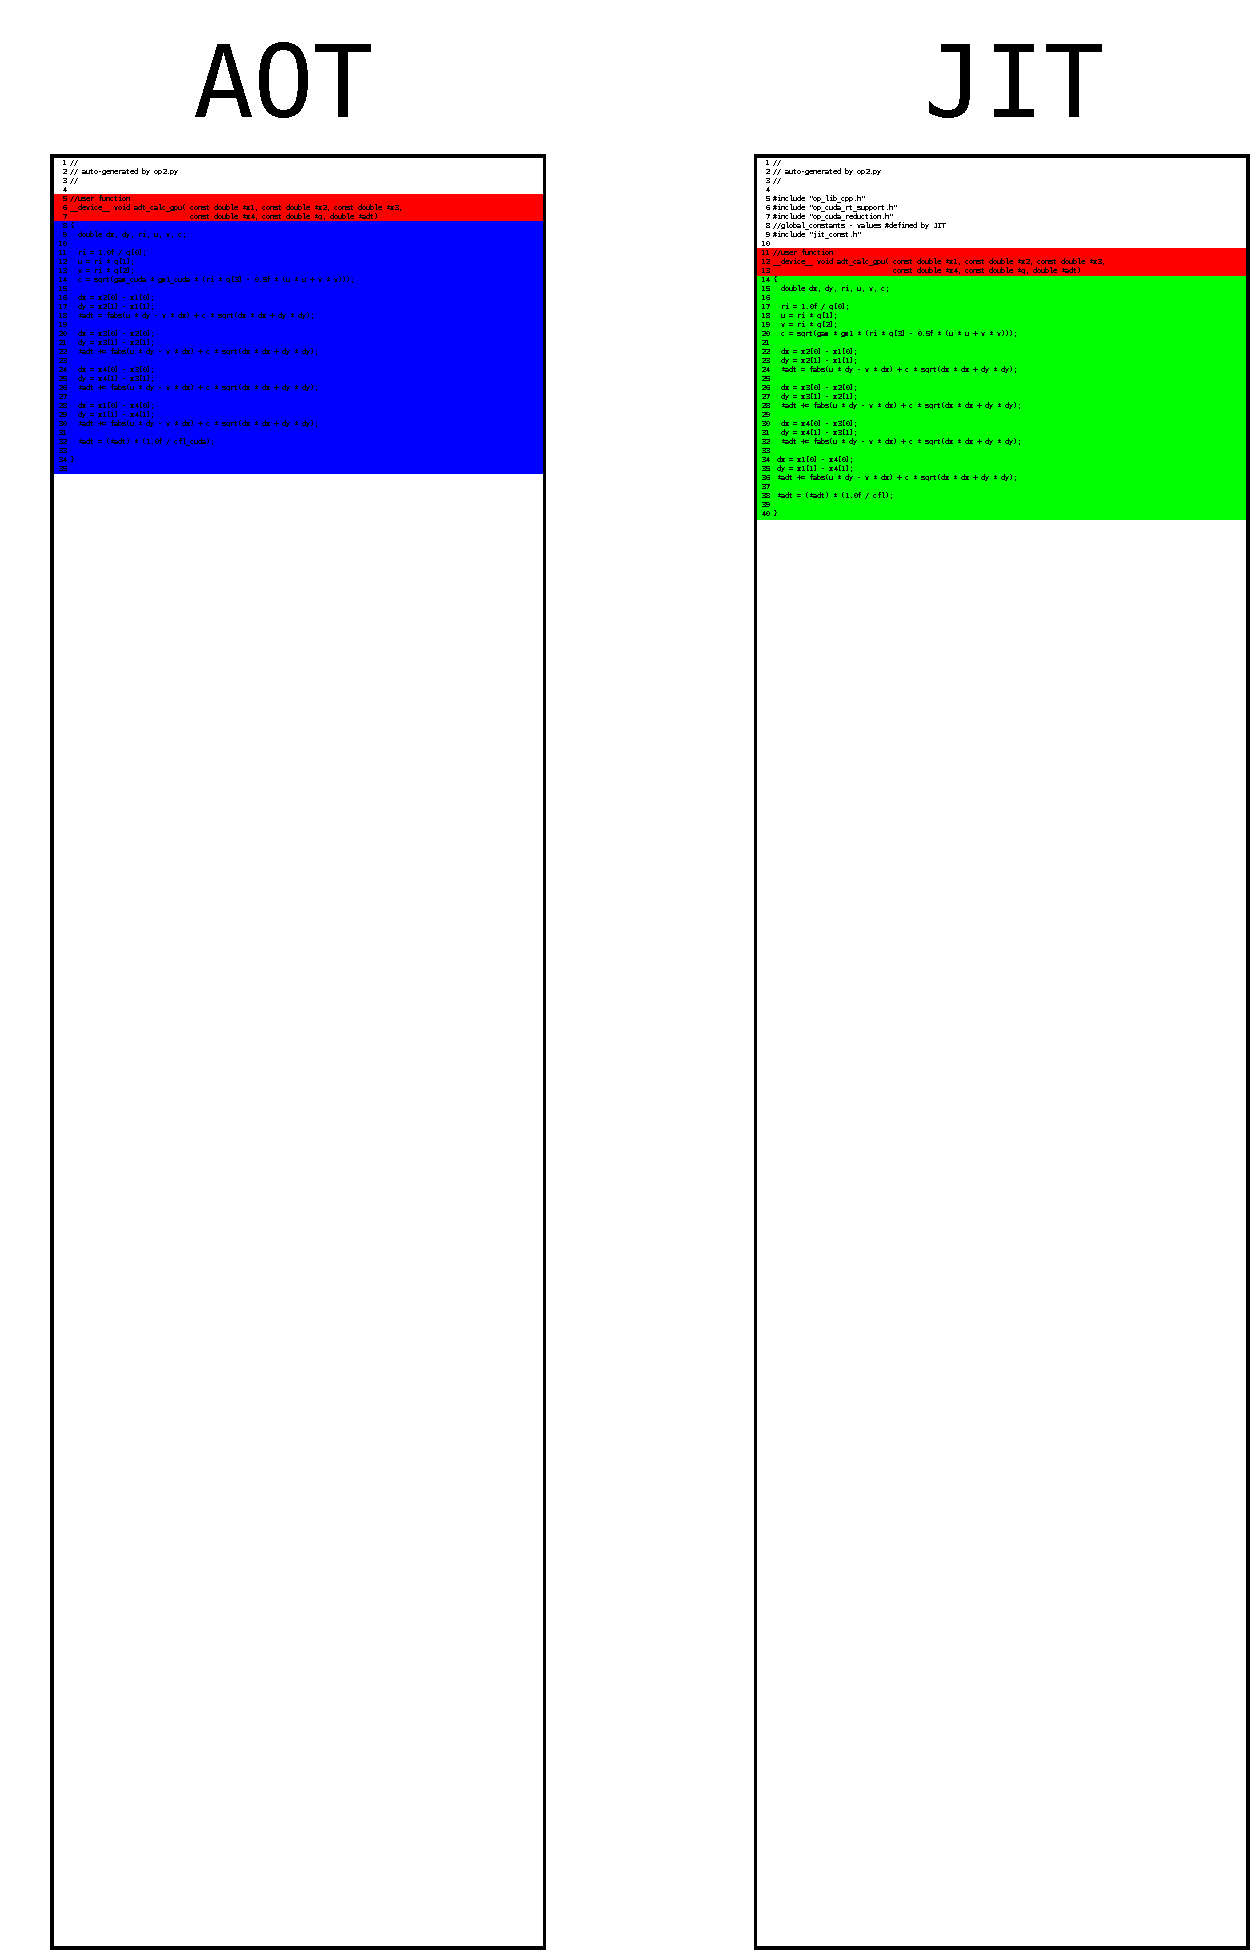
\includegraphics[width=.3\textwidth]{user_function}
\end{wrapfigure}
\minititle{User Function}
The User Function is the operation specified by the user to be carried out on each iteration of the loop. This function will run on the device (GPU) on many threads simultaneously, performing an action at least once for each set item.
\par
The User Function is given the \verb|__device__| function  descriptor, so that it will be compiled for execution on a GPU device, and so it can only be called from other device code - which will be the next function generated. The whole signature for the function will be:
\begin{lstlisting}[language=C, backgroundcolor=\color{red!20}]
__device__ void [name]_gpu ( [args] )
{
  ...
\end{lstlisting}
\codelabel{generated by TODO}

\noindent The function body is pulled from a function written by the application programmer, and found in the input files: either the Application File, or one of the optional header files. Once found, it needs to be checked to ensure it has the correct number of parameters, otherwise it is not valid to be used as the user function, and code generation will end with an error.
\par
Any \verb|#include| statements in the file containing the user function are replaced by the contents of the file, exactly as the pre-processor would do normally.
\par
\tinytitle{Data Layout} If the flag for automatic Struct-of-Arrays data layout transformation is not enabled, the function body will remain largely the same as defined by the application programmer. However, if it is enabled, there are modifications that need to be made to the function body to achieve this.
\par The code for making this transformation is pulled from the pre-existing AOT CUDA code generation script: \\\verb|translator/c/python/aot/op2_gen_cuda_simple.py|.
\par
The purpose of the code segment (\verb|op2_gen_cuda_jit.py| [242-257]) is to multiply array access indices by the stride for that data structure, which will be set as a constant later by the Host Function. If the access is indirect, it is the second index that is multiplied by the stride of the inner map.
\begin{figure}[h]
  \centering
  \subfloat[Array-of-Structs (AoS) layout]
  {
    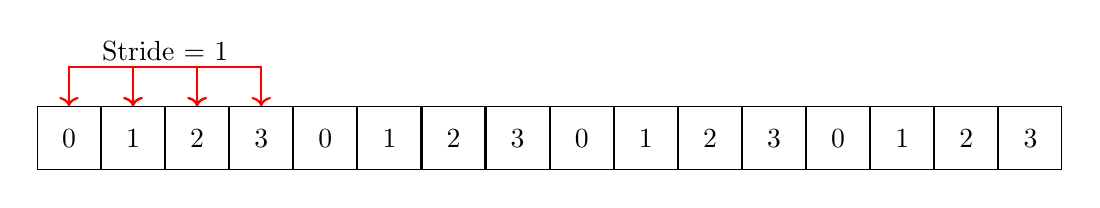
\begin{tikzpicture}[cell/.style={rectangle,draw=black}, ampersand replacement=\&, space/.style={minimum height=1.5em,matrix of nodes,row sep=-\pgflinewidth,column sep=-\pgflinewidth,column 1/.style={font=\ttfamily}},text depth=0.5ex,text height=2ex,nodes in empty cells]

    \tikzset{square arrow/.style={to path={-- ++(0,.5) -| (\tikztotarget)}}}

    \matrix (A) [matrix of nodes, nodes={draw, minimum size=8mm}]{
        \node (z) {0}; \& \node (o) {1}; \& \node (tw) {2}; \& \node (th) {3}; \& 0 \& 1 \& 2 \& 3 \& 0 \& 1 \& 2 \& 3 \& 0 \& 1 \& 2 \& 3\\};

    \draw[<->,square arrow, red, thick]
      (z.north) to (o.north) ;
    \draw[<->,square arrow, red, thick]
      (o.north) to (tw.north) ;
    \draw[<->,square arrow, red, thick]
      (tw.north) to (th.north) ;

    \node [above, yshift=2.5ex] at  ($(o.north)!0.5!(tw.north)$) {Stride = 1};

    \end{tikzpicture}
  }

  \quad

  \subfloat[Struct-of-Arrays (SoA) layout]
  {
    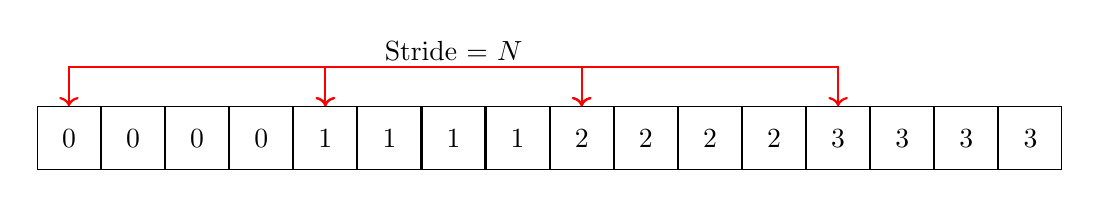
\begin{tikzpicture}[cell/.style={rectangle,draw=black}, ampersand replacement=\&, space/.style={minimum height=1.5em,matrix of nodes,row sep=-\pgflinewidth,column sep=-\pgflinewidth,column 1/.style={font=\ttfamily}},text depth=0.5ex,text height=2ex,nodes in empty cells]

    \tikzset{square arrow/.style={to path={-- ++(0,.5) -| (\tikztotarget)}}}

    \matrix (A) [matrix of nodes, nodes={draw, minimum size=8mm}]{
      \node (z) {0}; \& 0 \& 0 \& 0 \& \node (o) {1}; \& 1 \& 1 \& 1 \& \node (tw) {2}; \& 2 \& 2 \& 2 \& \node (th) {3}; \& 3 \& 3 \& 3\\};

    \node [above, yshift=2.5ex] at  ($(o.north)!0.5!(tw.north)$) {Stride = $N$};

    \draw[<->,square arrow, red, thick]
      (z.north) to (o.north) ;
    \draw[<->,square arrow, red, thick]
      (o.north) to (tw.north) ;
    \draw[<->,square arrow, red, thick]
      (tw.north) to (th.north) ;

    \end{tikzpicture}
  }
  \caption{\label{fig:SoA_v_AoS} Data layouts with labelled strides}
\end{figure}
\par

\tinytitle{Constant Definition} The Constant Definition optimisation needs to be applied to the user function, as it contains code written by the application developer. Wherever an input constant is referenced it needs to be modified in both the AOT and JIT kernel, but in different ways.

\tinytitle{AOT}
In the Ahead-Of-Time kernel, which will only be executed if JIT compilation is disabled, the constant will need to read from the device's memory - where the value will have been copied when it is defined as a constant. The copied version will have the identifier \verb|[id]_cuda| to prevent a name collision, so all constants in the AOT kernel must be replaced with this pattern, which is achieved by the following lines from the translator script:\\
\begin{lstlisting}[backgroundcolor = \color{lightgray!20}, language=Python]
for nc in range(0,len(consts)):
  varname = consts[nc]['name']identifier
  aot_user_function = re.sub('\\b' + varname + '\\b',
                              varname + '_cuda',
                              aot_user_function)
\end{lstlisting}
\codelabel{op2\_gen\_cuda\_jit.py [905-907]}

\tinytitle{JIT}
The JIT kernel needs to be modified differently. Constants with a dimension of 1 (i.e.\ they contain only 1 value) can be left unchanged, as the literal value will be defined under that same identifier. There is no possibility of a name collision here since the identifier will never be allocated memory, only replaced by a literal value.
\par
Constants with multiple values (i.e.\ with a dimension greater than one) cannot be defined as a macro, since macro values cannot have multiple values, and cannot be indexed. It also CUDA does not allow variables to be declared both \verb|__constant__|, and given external linkage using \verb|extern| \cite[p126]{guide}, which is how they are handled for the sequential JIT implementation.
\par
The solution to this challenge comes in two parts. For each index \verb|N| of the constant array, a 1 dimensional constant would be defined with the name:\\ \verb|op_const_[id]_[N]|. All references to the constant where the index is a literal number can be replaced with the new identifier:
\begin{lstlisting}[backgroundcolor = \color{lightgray!20}, language=Python]
for nc in range(0,len(consts)):
  varname = consts[nc]['name']
  if consts[nc]['dim'] != 1:
    jit_user_function = re.sub(`\\b' + varname + `\[([0-9]+)\]',
                               `op_const_' + varname + `_\g<1>',
                                jit_user_function)}
\end{lstlisting}
\codelabel{op2\_gen\_cuda\_jit.py [931-934]}

However, if the constant is accessed using any expression other than a integer literal, this system will run into an issue.
\par As an example, see the result of processing the following statement, where \verb|c_array| is a defined constant with dimension greater than 1:
\begin{center}
\lstinline|int A = c_array[1 + 2]| \hspace{1cm}$\Rightarrow$\hspace{1cm} \lstinline |int A = op_const_c_array_1 + 2|
\end{center}

If this problem is not solved the most likely outcome is an undefined identifier error at compile time. In the above example the code will compile without error, but the whole meaning of the statement has changed from the developer's intention, as \verb|op_const_c_array_1| will be replaced by the first value in the array, then the literal integer value of 2 will be added to it.
\par
To resolve this, a constant device array is declared in global scope above the top of the function, with the identifier \verb|op_const_[name]|. Each index of the array will be the constant defined for that position. The accesses can then still use the expression for an index, but are modified to instead access the new array, instead of the constant's identifier - so that the meaning of the statement is preserved.
\par This is only done when an expression index is found and the process becomes necessary, since allocating a new array can take time. If there are no expression accesses, the code will not be generated to handle them.\\
\begin{lstlisting}[backgroundcolor=\color{green!20}]
__constant__ int op_const_c_array = { op_const_c_array_1, ..._2, }
 ...
int A = op_const_c_array[1+2]
\end{lstlisting}
\codelabel{generated by TODO}

The above is a trivial example, and the actual code is unlikely to be an expression involving only literal values. If it were, then there would be benefit to implementing constant folding \cite{constFold} to evaluate the expression at compile time where possible, but this was not done due to the unlikely possibility of such code actually being written.
\clearpage
\noindent The full Python listing for generating C code to handle constants in JIT compiled kernel is provided below.
\begin{lstlisting}[backgroundcolor = \color{lightgray!20}, language=Python]
for nc in range(0,len(consts)):
  varname = consts[nc]['name']
  if consts[nc]['dim'] != 1:
    # Replace all instances with literal int index
    jit_user_function = re.sub('\\b'+varname+'\[([0-9]+)\]',
                               'op_const_'+varname+'_\g<1>',
                                jit_user_function)

    # Replace and count all remaining array accesses
    jit_user_function, numFound = re.subn('\\b'+varname+'\[',
                                          'op_const_'+varname+'[',
                                           jit_user_function)

    # At least one expression index was found
    if (numFound > 0):
      if CPP:
        #Line start
        codeline = '__constant__ '           +\
                    consts[nc]['type'][1:-1] +\
                   ' op_const_'              +\
                    varname                  +\
                   '[' + consts[nc]['dim'] + '] = {'

        #Add each constant index to line
        for i in range(0,int(consts[nc]['dim'])):
          codeline += "op_const_"+varname+"_"+str(i)+", "

        # Remove last comma, add closing brace
        codeline = codeline[:-2] + "};"

        #Add array declaration above function
        jit_user_function =  codeline +\
                            '\n\n'    +\
                             jit_user_function
\end{lstlisting}
\codelabel{op2\_gen\_cuda\_jit.py [931-944 UPDATE]}

\tinytitle{SoA optimisation}
Since the modifications to enable the Struct-of-Arrays data layout involve constant values for the stride of each data structures, an attempt to streamline this process using the Constant Definition optimisation was made during this project. It was unsuccessful, with a longer discussion later on the reasoning in a later section on the Host Function.
\par


\begin{wrapfigure}[13]{r}{.33\textwidth}
  \centering
  \caption{Kernel Function}
  \label{fig:krnl_func}
  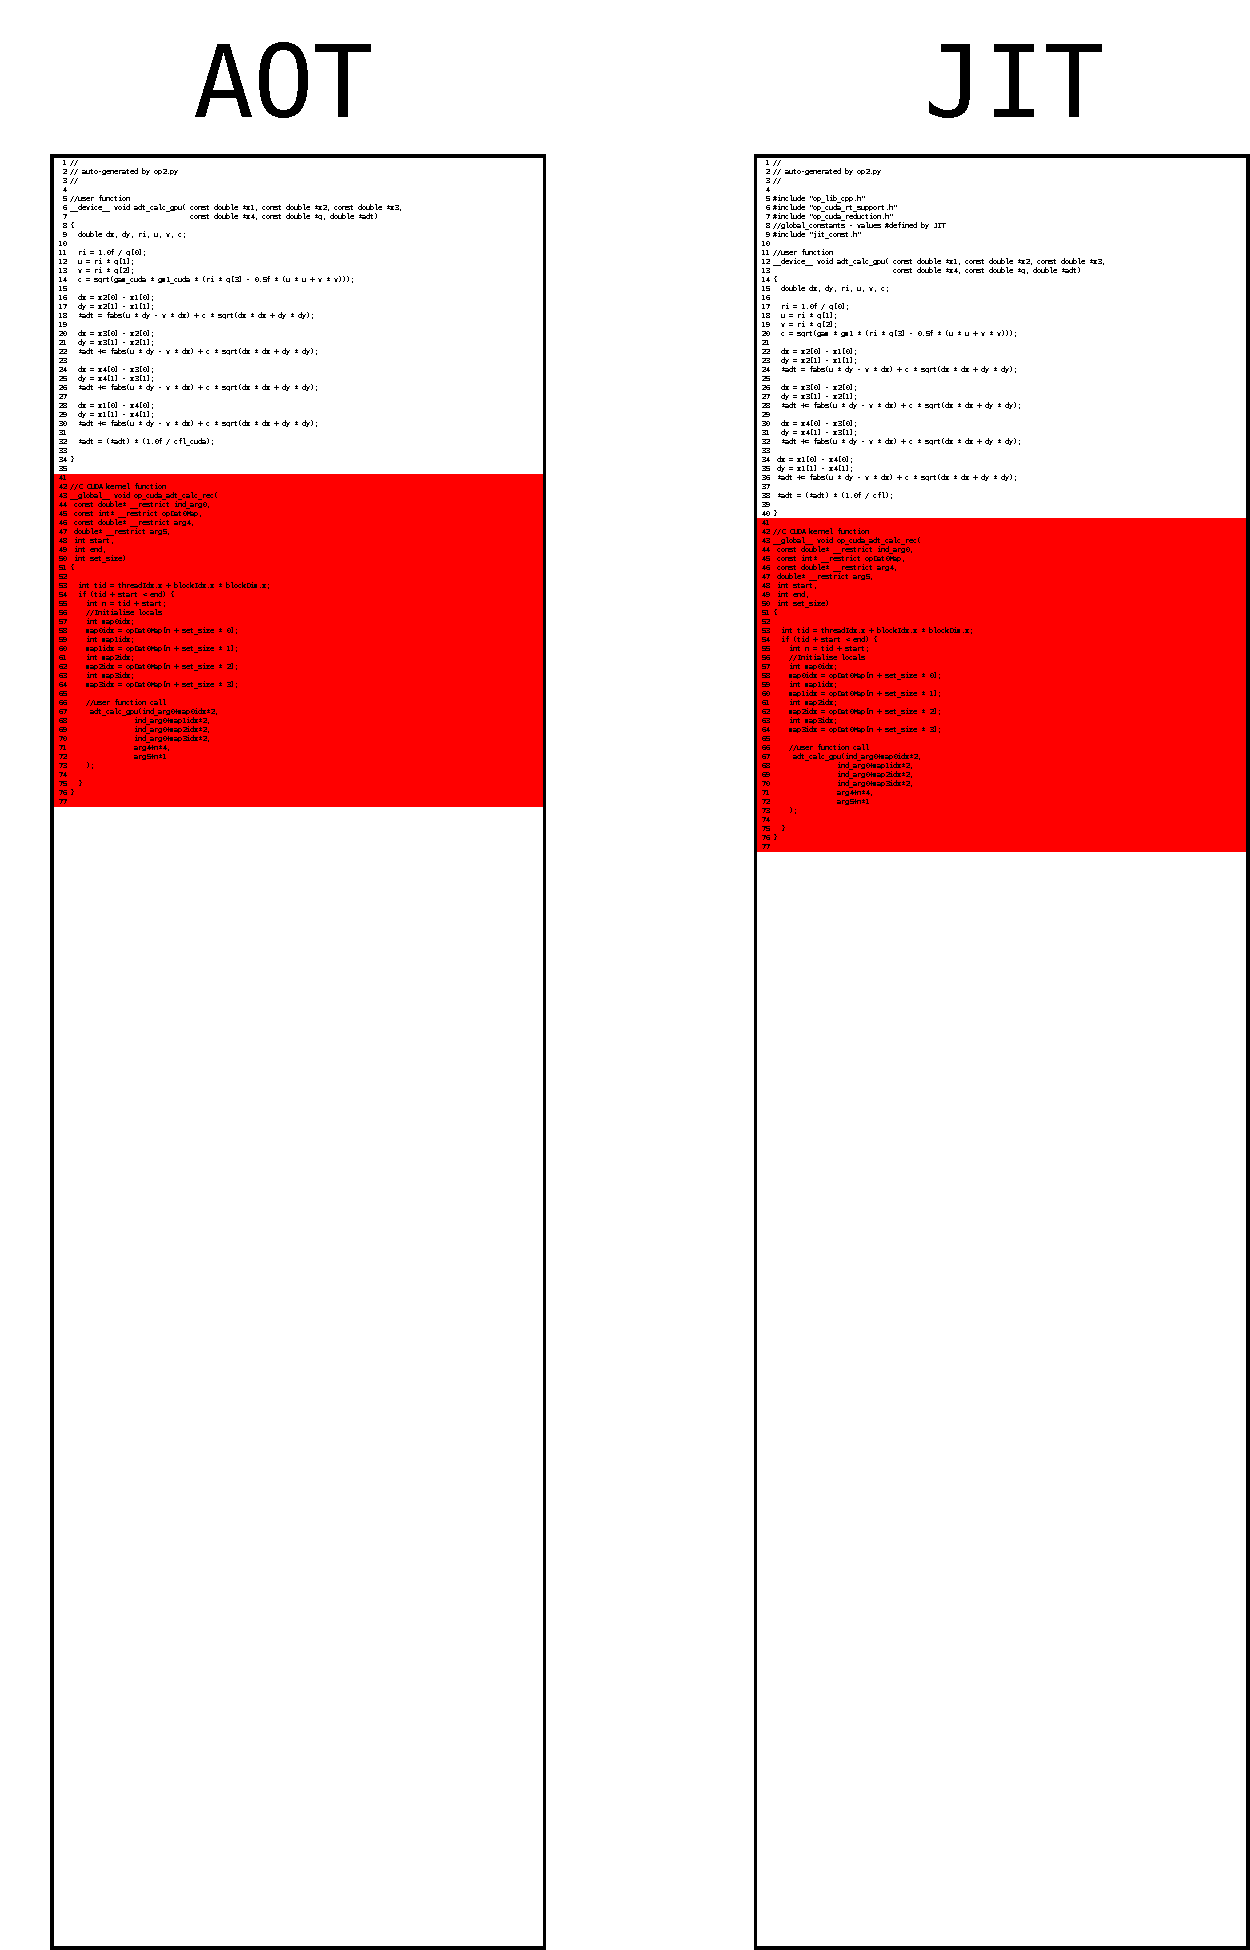
\includegraphics[width=.3\textwidth]{kernel_function}
\end{wrapfigure}
\minititle{Kernel Function}
From this section onwards, all code generated is based only on the kernel descriptor, and does not contain any code written by the application developer.
\par The kernel function is the same in both files, and is also executed on the GPU across all the parallel threads. It is declared \verb|__global__| so that is executed on the device, but can be called from host (CPU) code:
\begin{lstlisting}[language=C, backgroundcolor=\color{red!20}]
__global__ void op_cuda_'+name+'( [args] )
{
  ...
\end{lstlisting}
\codelabel{generated by op2\_gen\_cuda\_jit.py [TODO]}

\noindent The purpose of this function is to use the CUDA built in variables \verb|threadIdx.x|, \verb|blockIdx.x|, and \verb|blockDim.x| to map a unique portion of the workload onto each executing thread.

\tinytitle{Indirection} If the loop is indirect, and uses values from another map as indices, these values need to be read from the inner map in this function, so that the User Function (generated above) can receive all the data already formatted in the manner it expects to receive it. It is possible that the indirect map is optional, in which case the \verb|optflags| argument needs to be checked using a bit comparison, to determine if the optional argument was passed or not.
\par
Once this is done, a call is then made to the user function with the parameters it requires, followed by performing any data reductions necessary. The supported reductions are: sum, maximum, and minimum \cite[p11]{manual}. Reductions are handled by the \verb|op_reduction| library function.

\begin{wrapfigure}[10]{r}{.33\textwidth}
  \centering
  \caption{Host Function}
  \label{fig:host_func}
  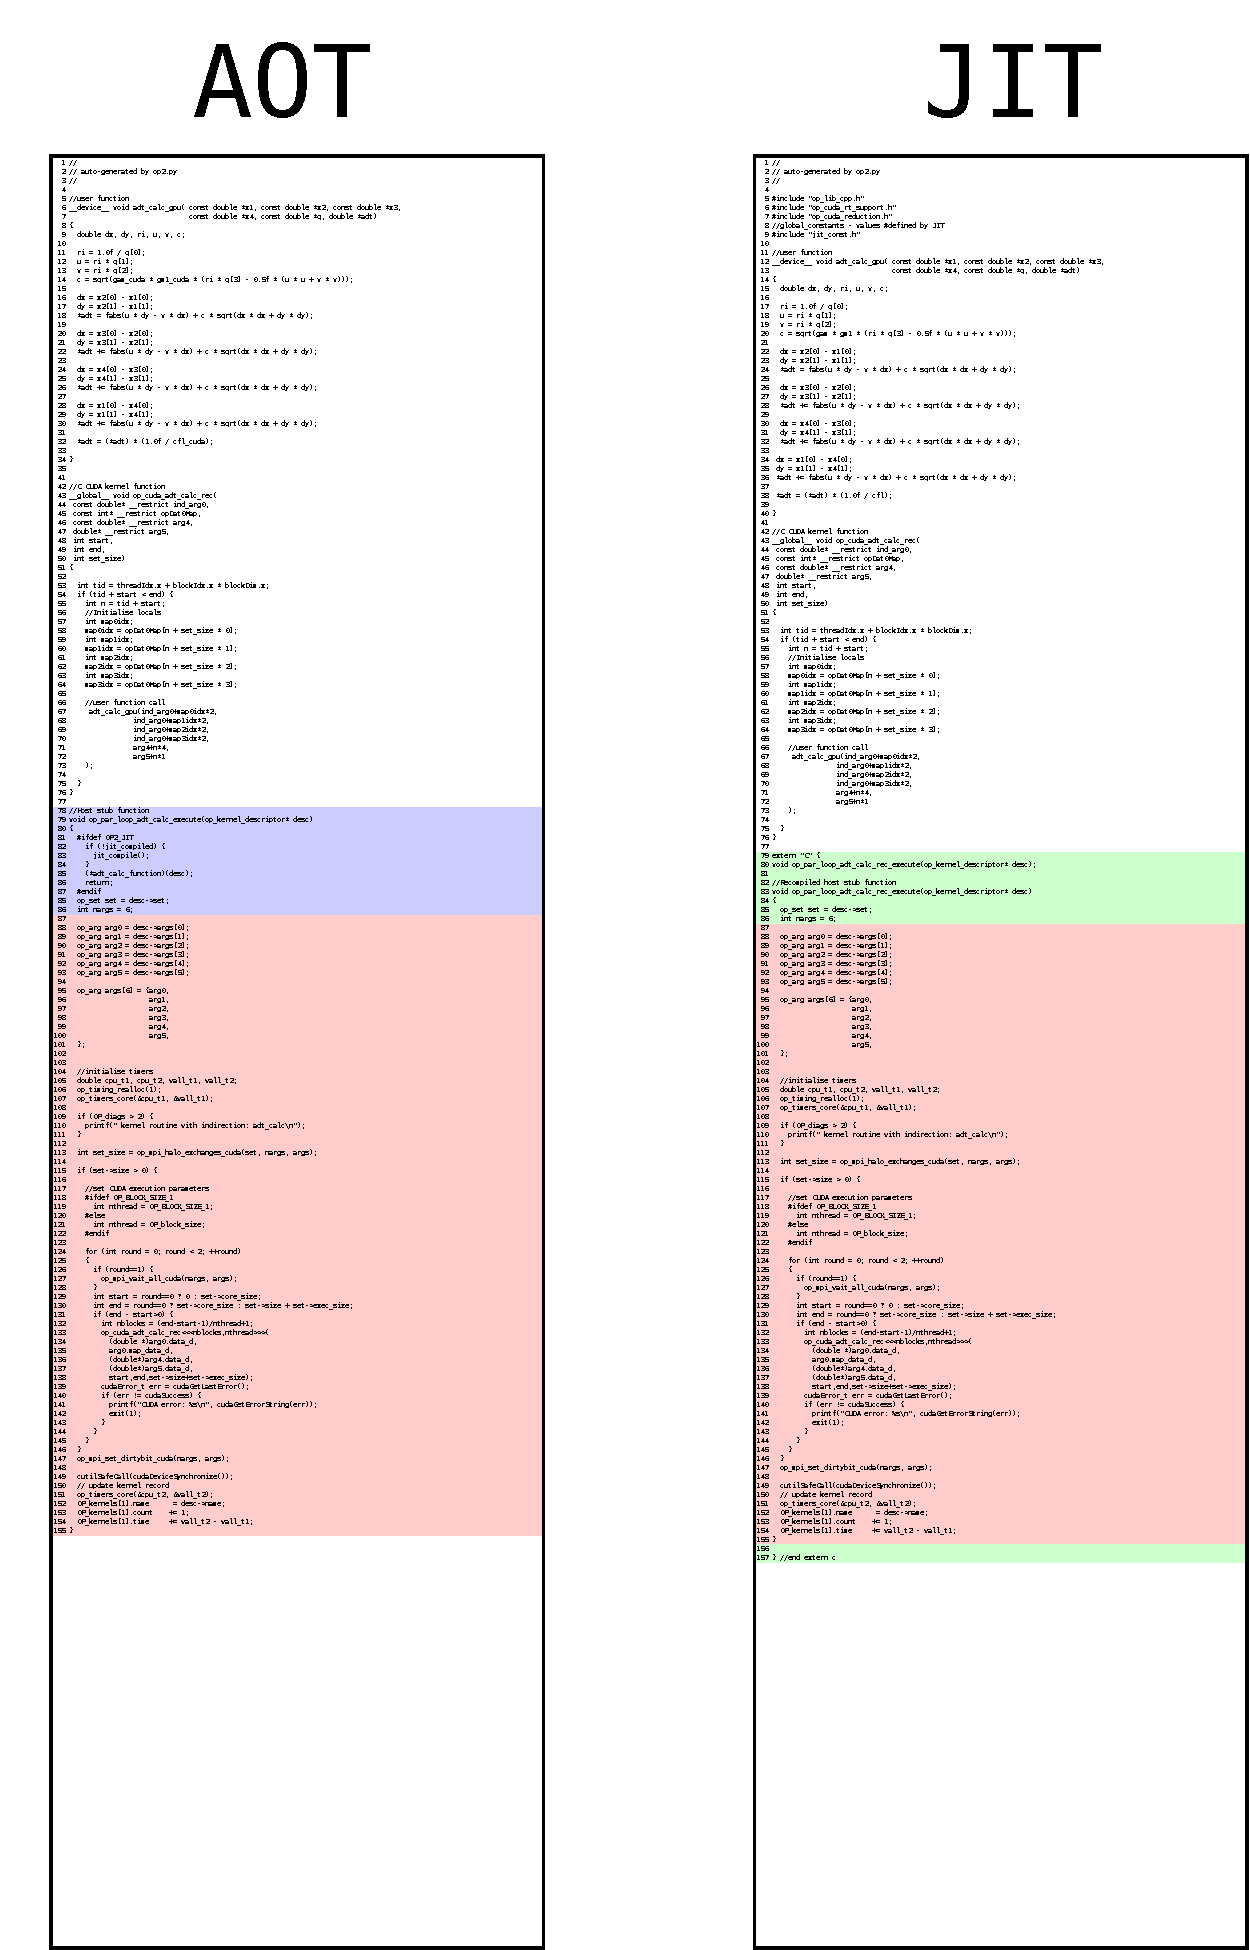
\includegraphics[width=.3\textwidth]{host_function}
\end{wrapfigure}
\minititle{Host Function}
The purpose of the host function is to bridge the gap between the host and the device. It is CPU code, so runs on the host, but contains the CUDA call to the kernel function which will run in parallel on the GPU. The function body is the same for both AOT and JIT: setting up function arguments, block and thread sizes for the CUDA call, and timers to record how long is spent in each parallel loop. The head of the function does differ however, as highlighted in Figure \ref{fig:host_func}.
\vspace{\parskip}

\tinytitle{AOT}
In the Ahead-Of-Time kernel file, the C code generated for the head of the host function is as follows:

\begin{lstlisting}[linewidth = \textwidth, framesep=0pt, language=C, linebackgroundcolor={\ifnum\value{lstnumber}<15 \ifnum\value{lstnumber}>10 \color{red!20} \else \color{blue!20} \fi \else \color{blue!20} \fi}]
 //Host stub function
 void op_par_loop_[name]_execute(op_kernel_descriptor* desc)
 {
   #ifdef OP2_JIT
     if (!jit_compiled) {
       jit_compile();
     }
     (*[name]_function)(desc);
     return;
   #endif

   op_set set = desc->set;
   int nargs = 6;
   ... //Identical Section
 }
\end{lstlisting}

\codelabel{Generated by jit/op2\_gen\_cuda\_jit.py [537-558]}

The function name is \verb|op_par_loop_[name]_execute| because a pointer to this function will be queued by the lazy execution system mentioned previously in this Section, so this function actually executes the loop, whenever the lazy execution system should decide it needs to be executed. The decision of when to call the loop is outside the scope of this project, as it would be part of the lazy execution feature, but currently the loop will simply be called immediately after it is queued.
\par At the top of the function a decision is made as to whether JIT compilation should be used, based on whether the pre-processor flag: \verb|OP2_JIT| has been defined. This allows JIT compilation to be enabled by passing the compiler argument \verb|-DOP2_JIT|, and otherwise by default it will be disabled. If JIT compilation is enabled, then the compiler is invoked if this execution is the first of the application, then the pointer to the newly compiler version of the function is executed instead.
\par
The actual invocation of the compiler process is handled by the \verb|jit_compile()| function, which has not yet been generated, as it will reside in the central kernels file. It will be discussed in detail, along with the other functions in that file, in Section \ref{sss:mkf}.
\par
If JIT is not enabled, the lines of code between \verb|#ifdef| and \verb|#endif| will be ignored by the compiler, so the process will continue into the AOT host function, which causes it to stay within the AOT kernel file and never execute any code from the JIT file.
\par
The pre-processor condition section is generated using the following Python code:
\begin{lstlisting}[backgroundcolor=\color{lightgray!20}, language=Python]
    code('#ifdef OP2_JIT')
    depth += 2
    IF("!jit_compiled")
    code('jit_compile();')
    ENDIF()
    code('(*'+name+'_function)(desc);')
    code('return;')
    depth -= 2
    code('#endif')
    code('')
\end{lstlisting}
\codelabel{op2\_gen\_cuda\_jit.py [546-555]}



\tinytitle{JIT}
The code generated for the top of the Host Function in a JIT kernel file is shown below. Contrasting with the code generated for the AOT kernel file there are a few key differences. Firstly, since this function needs to be linked to the existing code as part of a dynamically loaded library, it is placed inside an \verb|extern "C"| scope, to ensure C language function linkage, and prevent the compiler from "mangling" the name as it would for C++ code \cite{linkage}.

\begin{lstlisting}[linewidth = \textwidth, framesep=0pt, linebackgroundcolor={\ifnum\value{lstnumber}<10 \ifnum\value{lstnumber}>6 \color{red!20} \else \color{green!20} \fi \else \color{green!20} \fi}]
 extern "C" {
 void op_par_loop_[name]_rec_execute(op_kernel_descriptor* desc);

 //Recompiled host stub function
 void op_par_loop_[name]_rec_execute(op_kernel_descriptor* desc)
 {
   op_set set = desc->set;
   int nargs = 6;
   ... //Identical Section
 }

 } //end extern c
\end{lstlisting}

\codelabel{Generated by op2\_gen\_cuda\_jit.py [522-531]}

\noindent As can be seen above, the function also has a different signature:\vspace{1em}
\begin{lstlisting}[backgroundcolor=\color{green!20}, language=C]
op_par_loop_[name]_rec_execute(op_kernel_descriptor* desc)
\end{lstlisting}
\vspace{-1em}
Instead of:
\vspace{.5em}
\begin{lstlisting}[backgroundcolor=\color{blue!20}, language=C]
op_par_loop_[name]_execute(op_kernel_descriptor* desc)
\end{lstlisting}
As before, ``rec" is short for \textbf{recompiled}. This version of the function will come to reside at the address pointed to by the \verb|[name]_function| function pointer previously referenced in the AOT kernel. It will be executed after the run-time compiler has been invoked, by the following line from the code listing on the previous page:

\begin{lstlisting}[backgroundcolor=\color{blue!20}, language=C]
     (*[name]_function)(desc);
\end{lstlisting}

\noindent Since it resides in the JIT kernel file, it makes calls to the Kernel Function and User Function in the same file as itself, rather than those in the AOT file, and as such the optimisations made to the User Function in the JIT kernel file are able to be used.

\tinytitle{SoA}
If the Struct-of-Arrays Data layout is enabled, the body of this function in both AOT compiled and JIT compiled kernels will need to set the stride length for each data structure and copy it to a CUDA device symbol. This is only done on the first iteration of each loop.
\begin{lstlisting}[linewidth = \textwidth, framesep=0pt,escapechar=:, language=C,backgroundcolor=\color{red!20}]
if ((OP_kernels[_].count==1) ||
    (direct_[name]_stride_OP2HOST != getSetSizeFromOpArg(&arg_)))
   )
   {
     direct_[name]_stride_OP2HOST = getSetSizeFromOpArg(&arg_);
     cudaMemcpyToSymbol( direct_[name]_stride_OP2CONSTANT,
                         &direct_[name]_stride_OP2HOST,
                         sizeof(int));
   }
\end{lstlisting}

\codelabel{Generated by op2\_gen\_cuda\_jit.py [640-654]}

\noindent These sizes only become available when the function has been called and it's arguments are known. As previously mentioned, an attempt was made to replace these constants with defined literal values in the JIT kernel, however this proved difficult as each loop would need to have been called at least once so that all the strides are known before the compilation could be done.
\par
For this to be possible, each loop would need to execute correctly before JIT compilation as well as after in the binary with JIT compilation enabled, and therefore all the input constants would need to be copied to device memory as usual, otherwise they would not be available before the re-compilation is initiated. This would add extra duration to the upfront cost of the optimisation.\par
Furthermore, parallel loops may not all be created equally. It is a possibility that a certain loop never gets called, or is only called for the first time half way through an application. In a situation such as that, any benefit that could be gained from JIT compiling would be wasted while waiting for every loop to have been called at least once.
\par
For this reason, the data structure strides remain as a device constant which is copied to device memory on the first iteration of a loop in both AOT compiled and JIT compiled kernels

\clearpage

\begin{wrapfigure}{r}{.33\textwidth}
  \centering
  \caption{Loop Function}
  \label{fig:loop_func}
  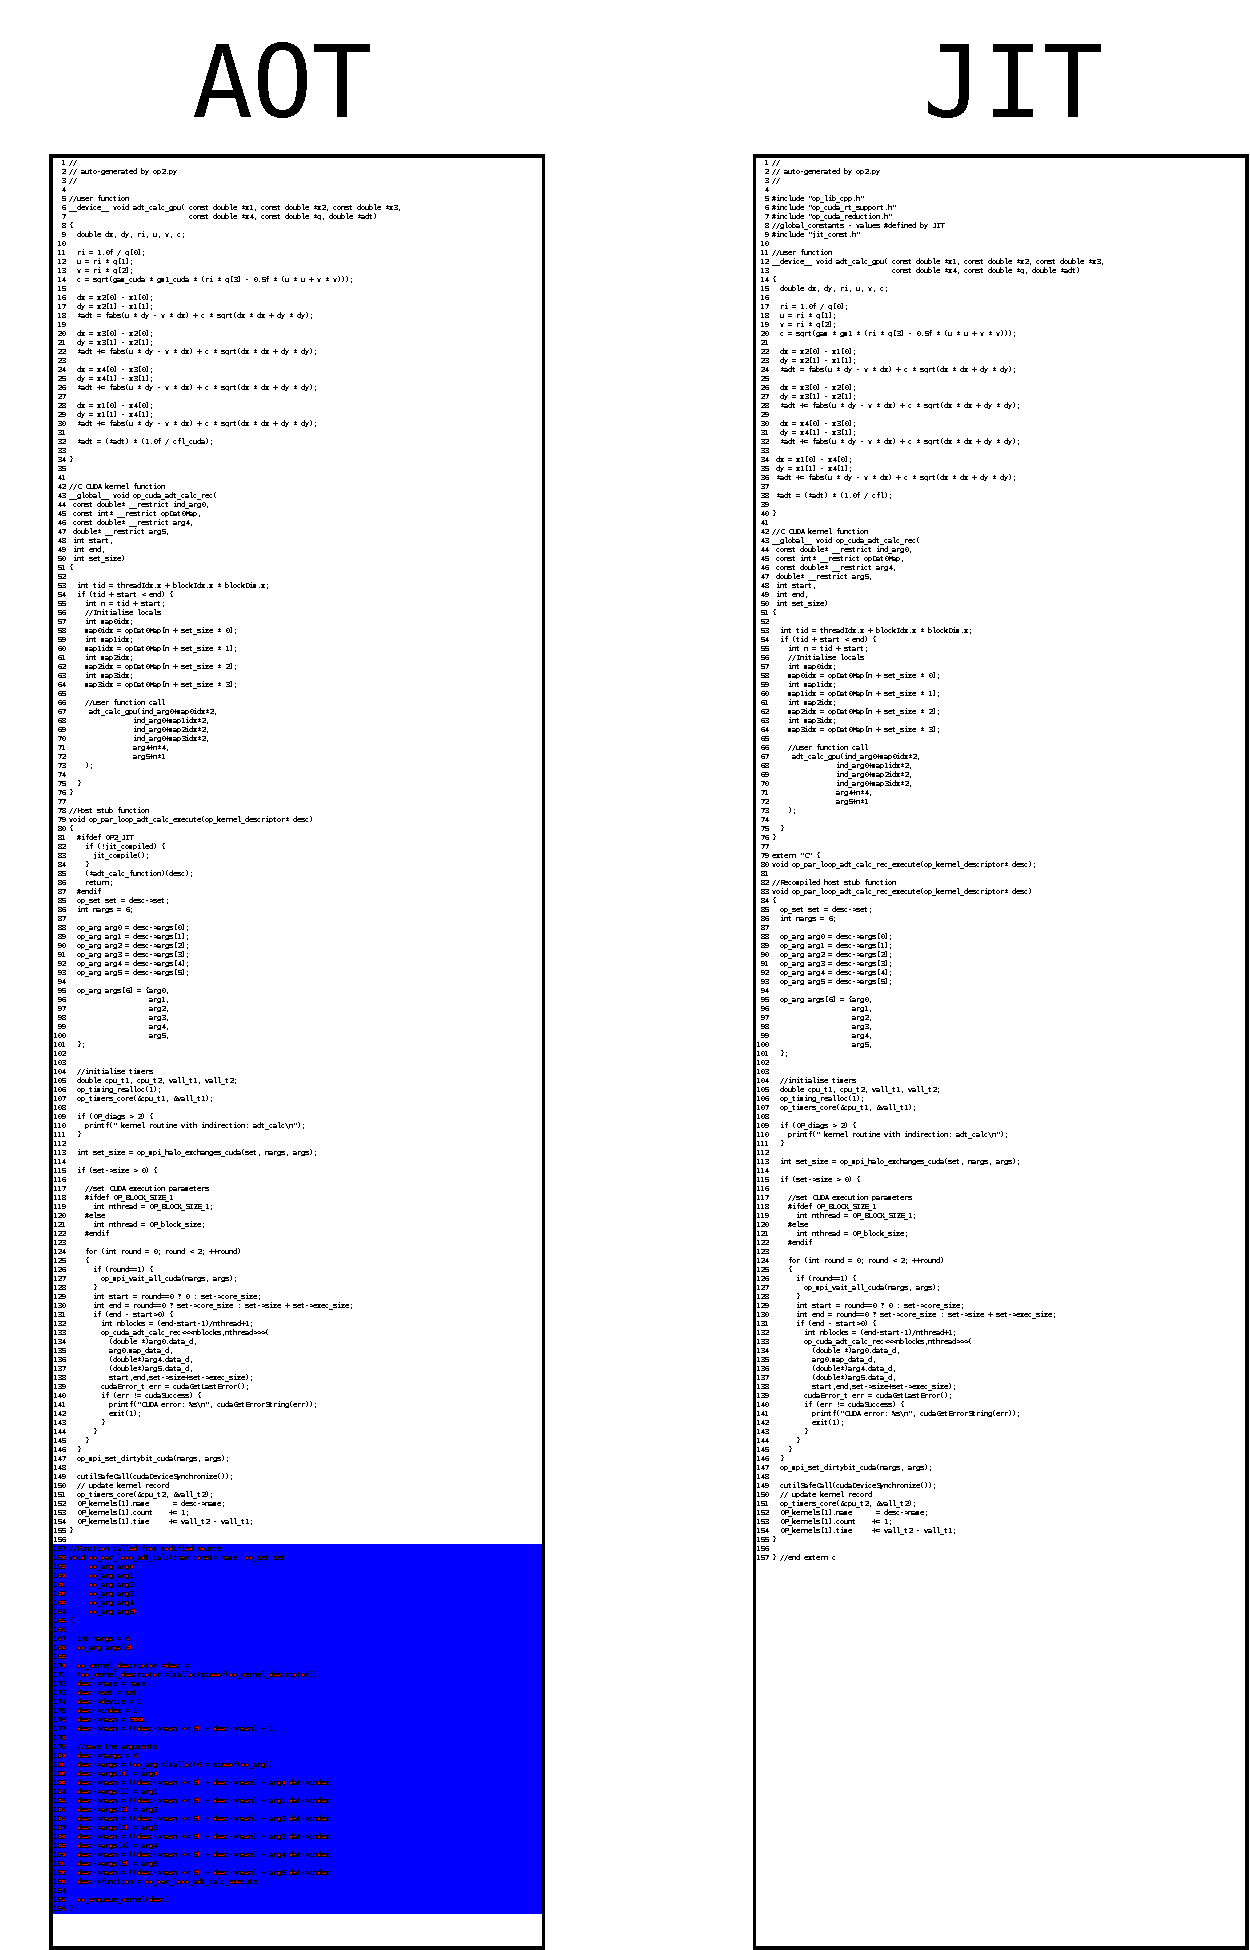
\includegraphics[width=.3\textwidth]{loop_function}
\end{wrapfigure}
\minititle{Loop Function}
The last section to be added to the kernel files for each parallel loop is the Loop Function, which serves as the entry point for the whole loop operation.
 \par
The Application File will be modified by \verb|op2.py| to contain an declaration for this function marked \verb|extern|, to be linked against this definition in the CUDA version of the executable. Only the AOT kernel requires this function, as the Host Function acts as the entry point for the JIT compiled kernel The function signature is:
\begin{lstlisting}[backgroundcolor=\color{blue!20}, language=C]
void op_par_loop_[name](char* name, op_set set, ...)
{

\end{lstlisting}
\codelabel{generated by op2\_gen\_cuda\_jit.py [878]}
\par
\noindent The purpose of the Loop Function is to generate the kernel descriptor for the loop. This is an OP2 data structure that contains the name, operating set, arguments, and execution function of the loop, and is passed as an argument to the enqueue function so it can be executed at a time decided by the lazt execution subsystem:
\codeline{void op_enqueue_kernel(op_kernel_descriptor *desc)}{op2/c/src/core/op\_lazy.cpp [71-89]}

\noindent As previously mentioned, the kernel descriptor and enqueue function were part of the work done to enable lazy execution in OP2, and not created as part of this project.

\clearpage

\subsubsection{Kernel Files Summary}
\label{impl_summary}

To summarise, for every parallel loop two separate kernel files containing C and CUDA code are generated, one for Ahead of Time compilation, and one for Just in Time compilation. The generated code in a particular pair of kernel files will to be executed when the corresponding loop is invoked in the Application File, which has been modified so that the compiler will link its function calls to the function definitions generated above.

\begin{wrapfigure}{r}{.42\textwidth}
  \centering
  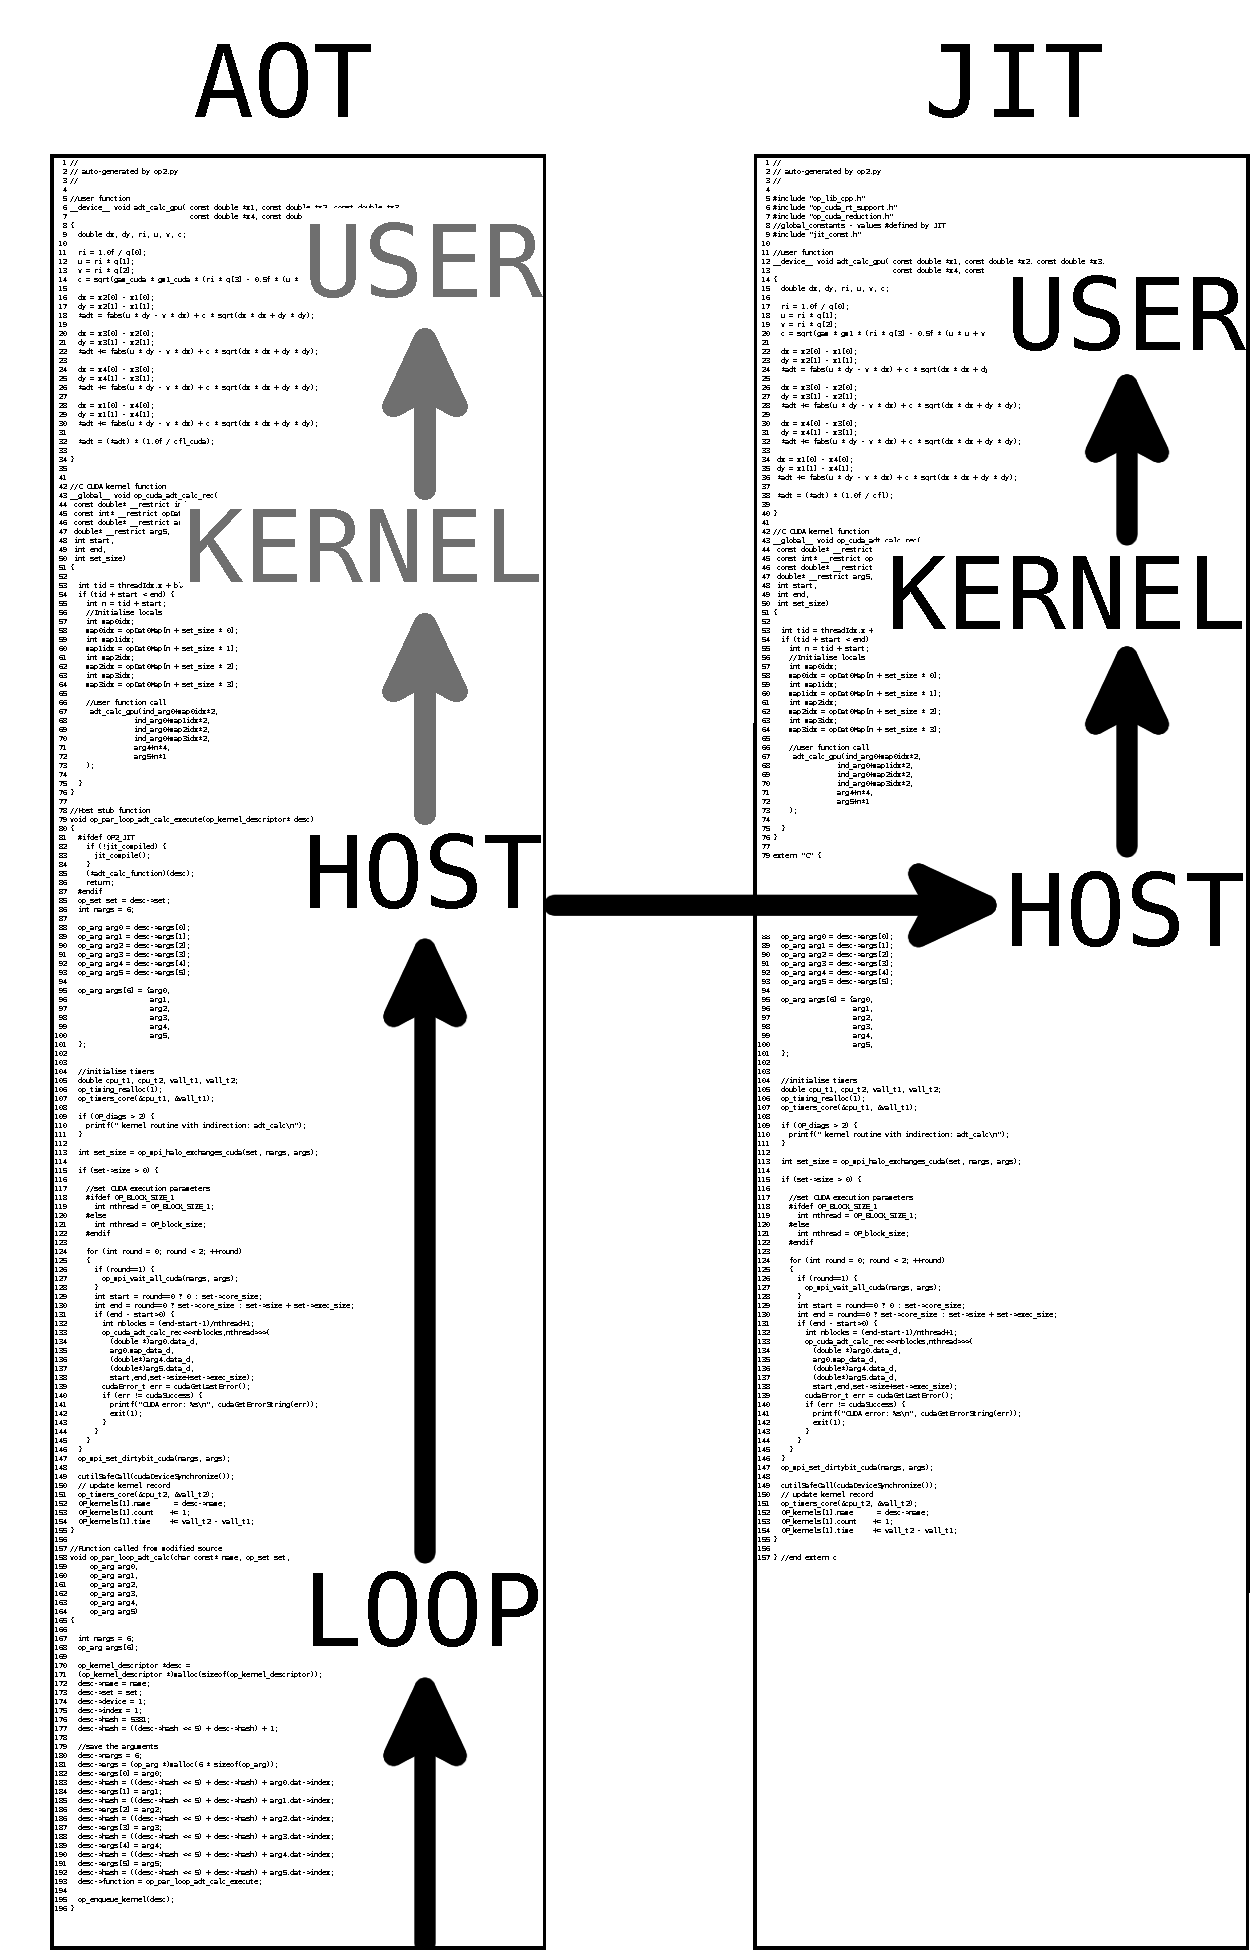
\includegraphics[width=.39\textwidth]{krnl_flow}
  \caption{Kernel Flow}
  \label{fig:krnl_flow}
\end{wrapfigure}

Figure \ref{fig:krnl_flow} has been included to clarify the data flow through the two files, where an arrow from Function A to Function B indicates that B is called from the body of A. The diagram starts with the Loop Function at the bottom which is called from the Application File, and executed by a single thread on the host. The AOT Host Function is eventually called, where either the re-compiled JIT version is invoked, or the original version is used if JIT compilation is not enabled when the application is first compiled. In the host function the GPU device is configured, and Kernel Function is executed simultaneously on many parallel threads. Each thread in turn executes the User function to perform an operation on elements of a set, as per the design of the application programmer.

The \verb|jit_compile()| function, which will handle actually performing a compilation stage at runtime, has not yet been defined. This will be covered in the next section on the final source file to be generated: the Central Kernels file.
\clearpage
\subsubsection{Central Kernels File}
\label{sss:mkf}
The Central Kernels File resides in the \verb|cuda/| directory alongside the Kernel files. It is named: \verb|cuda/[application]_kernels.cu| and is the final source file to be generated, once the Kernel files for each parallel loop are complete. It will tie up the remaining loose ends, as it contains the \verb|jit_compile()| function for invoking the run-time compiler, and the definition for the new OP2 API function for declaring constants.
\par It also contains \verb|#include| statements for each of the AOT kernel files, so that their contents is imported to make a single file, and can be compiled in a single parse. The compilation process for generated code will be covered further in Section \ref{ss:make} on the Makefile.
\par
At the top, the central kernels file includes the required OP2 library files, as seen at the very start of this Section for the JIT compiled kernel:
\begin{lstlisting}[backgroundcolor = \color{red!20}, language=C]
\\header
 #include `op_lib_cpp.h'
 #include `op_cuda_rt_support.h'
 #include `op_cuda_reduction.h'
 ...
\end{lstlisting}
\codelabel{generated by TODO}
As mentioned in that section, these serve as a reference to the OP2 library files for all of the AOT kernels, and their inclusion here is the reason the AOT kernels do not each individually require these statements.

A declaration of a CUDA constant for each input constant in the user's dependingn is generated next. An example of what this might look like is shown below.
\begin{lstlisting}[backgroundcolor=\color{red!20}, language=C]
__constant__ double single_cuda;
__constant__ double value_cuda;
__constant__ double constant_cuda;
__constant__ double four_vals_cuda[4];
\end{lstlisting}
\codelabel{generated by op2\_gen\_cuda\_jit.py [1026-1037]}

These declarations are generated using the following Python code.
\begin{lstlisting}[backgroundcolor = \color{lightgray!20}, language=Python]
for nc in range (0,len(consts)):
  if consts[nc]['dim']==1:
    # __constant__ [type] [name]_cuda;
    code('__constant__ ' + consts[nc]['type'][1:-1] + ' ' +
          consts[nc]['name'] + '_cuda;')
  else:
    if consts[nc]['dim'] > 0:
      num = str(consts[nc]['dim'])
    else:
      num = 'MAX_CONST_SIZE'

    # __constant__ [type] [name]_cuda[ [dim] ];
    code('__constant__ ' + consts[nc]['type'][1:-1] + ' ' +
          consts[nc]['name'] + '_cuda' + '['+num+'];')
\end{lstlisting}
\codelabel{op2\_gen\_cuda\_jit.py [1026-1037]}

Following this, the file contains definitions for two functions. The first is the OP2 API function \verb|op_decl_const_char|, which will be called from the Application File when the programmer wishes to declare a constant identifier and value in the input; and the second is \verb|jit_compile| which will invoke the run-time compiler, load the generated shared object file, and assign a function pointer for each re-compiled loop exported by the DLL so it can be retrieved and executed when required.

\minititle{op\_decl\_const\_char}
This function is an OP2 API function which allows users to declare an input value that will not change over the course of execution. It currently has the following signature, as defined in the OP2 User Guide \cite[p9]{manual}:
\codeline{void op_decl_const_char(int dim, char const *type, int size,
                                  char *dat, char const *name)}{}
This signature will not be altered to ensure backwards compatibility. Fortunately, it does not need to be modified for the requirements of this project, so this is not an issue.
\par
Two versions of the function are generated, but only one will be needed depending on whether JIT compilation is enabled or disabled. To achieve this, the two function definitions are wrapped with pre-processor conditionals, so that only one of them will be visible to the compiler. As before, the \verb|OP2_JIT| flag being defined is the condition for the JIT functionality to be enabled.
\begin{lstlisting}[backgroundcolor=\color{red!20}, language=C]
#ifndef OP2_JIT

void op_decl_const_char(int dim, char const *type,
                        int size, char *dat,
                        char const *name)
{
  ... //JIT disabled function definition
}

#else

void op_decl_const_char(int dim, char const *type,
                        int size, char *dat,
                        char const *name)
{
  ... //JIT enabled function definition
}
...
void jit_compile() {
  ...
}

#endif
\end{lstlisting}
The \verb|jit_compile()| function is also wrapped by the pre-processor conditional, as it is only going to be required if JIT compilation is enabled. Although it would not detriment the program to include it in both versions, it is not necessary.

\tinytitle{AOT} The top version of the function, for when JIT compilation is disabled, is based on the existing code generation, and therefore copies the constant value passed to it to the device constant using a CUDA function for moving a value between host memory and device memory:
\codeline{cudaMemcpyToSymbol(const void* symbol, const void* src, size_t count)}{}
\noindent The default copy direction for this function is from host memory to device memory, so it does not need to be passed as a parameter.

\tinytitle{JIT}
The JIT version instead invokes the OP2 internal library function:
\codeline{void op_lazy_const(int dim, char const *type, int typeSize, char *data,
                        char const *name)}{op2/c/src/core/op\_lazy.cpp [100-101]}
\noindent This function was added with lazy execution, and maintains a de-duplicated list of constants, so that once they all have been declared the header file defining each value can be generated. As can be seen in the generated C code below, constants containing more than one value are iterated over, and each element is declared as asingle value due to the issues with \verb|extern __constant__| values described in Section \ref{ss:krnl_files} (2. User Function).
\begin{lstlisting}[backgroundcolor=\color{red!20}, language=C]
#else

void op_decl_const_char(int dim, char const *type,
                        int size, char *dat,
                        char const *name)
{
  if (dim == 1) {
    op_lazy_const(dim, type, size, dat, name);
  }
  else {
    for (int d = 0; d < dim; ++d)
    {
      char name2[32];
      sprintf(name2, "op_const_%s_%d\0", name, d);
      op_lazy_const(1, type, size, dat+(d*size), name2);
    }
  }
}
...
\end{lstlisting}
\vspace{-1em}
\codelabel{generated by op2\_gen\_cuda\_jit.py [1092-1114]}

\minititle{jit\_compile()}
The other function generated is the \verb|jit_compile()| function, which is responsible for the actual recompilation of the JIT kernels, and making their functions available to the binary. It also uses the same OP2 library functions for timing which kernel files used previously to gather data on the time spent in each parallel loop, as the time spent re-compiling the binary is important for performance comparisons later.
\par
Above the \verb|jit_compile()| function, in global scope, a function pointer is declared for each parallel loop, and defined \verb|NULL| so that after re-compiling the new version of the function can be referenced using the function pointer.

\begin{lstlisting}[backgroundcolor=\color{lightgray!20}, language=Python]
code('')
comm(' pointers to recompiled functions')
for nk in range (0,len(kernels)):
  name = kernels[nk]['name']
  code('void (*' + name +\
       '_function)(struct op_kernel_descriptor *desc) = NULL;')
\end{lstlisting}
\codelabel{op2\_gen\_cuda\_jit.py [1016-1120]}
\noindent The output of this Python code is a number of lines of C with the following form:
\begin{lstlisting}[backgroundcolor=\color{red!20}, language=C]
// pointers to recompiled functions
void (*[name]_function)(struct op_kernel_descriptor *desc) = NULL;
void (*[name]_function)(struct op_kernel_descriptor *desc) = NULL;
void (*[name]_function)(struct op_kernel_descriptor *desc) = NULL;
...

void jit_compile() {
\end{lstlisting}
\codelabel{generated by op2\_gen\_cuda\_jit.py [1016-1120]}

\tinytitle{Invoking the Compiler}\\
As can be seen below, the compiler is invoked by the executable through a system call to initiate a GNU Make \cite{make} command. It is expected that the Makefile is accessible at runtime as well as at compile time, and that it contains a target named \verb|[application]_cuda_rec| which will perform the necessary compilation. Furthermore, the compiler arguments, library install paths, and other parameters of the compiler are handled by the Makefile. The contents of the Makefile for this implementation will be covered in Section \ref{ss:make}.\par
Once the compilation has completed, the terminal output of the command is stored in a log file in case of an error, which will also cause an error message is printed, and the program to exit early.
\clearpage
\noindent This is the C code generated to perform the compilation, with error checking.
\vspace{1em}
\begin{lstlisting}[backgroundcolor=\color{red!20}, language=C]
if (op_is_root()) {
  if (system("make -j [application]_cuda_rec &> jit_compile.log"))
  {
    // 0 indicated success
    printf("Error: JIT compile failed. \n
            - see jit_compile.log for details\n");
    exit(1);
  }
}
\end{lstlisting}
\codelabel{generated by op2\_gen\_cuda\_jit.py [1139-1146]}
\par
\noindent It is expected that the result of the compilation will be a shared object file named\\ \verb|cuda/airfoil_kernel_rec.so|, which exports functions for each parallel loop. If this file does not exist the application binary will exit with an error, otherwise the recompiled function for each parallel loop is dynamically loaded into the application, using: \verb|void *dlsym(void *restrict handle, const char *restrict name)|\\ from \textit{dlfcn.h}.
\par
\noindent For every parallel loop, the function \verb|op_par_loop_[name]_rec_execute| is imported, with its address stored in the void pointer declared in global scope: \verb|[name]_function|. We have seen this pointer before, in Section \ref{ss:krnl_files}, where is was used to call the JIT kernel Host Function from the AOT kernel Host Function.
\par
The value return from \verb|dlsym()| needs to be cast to the type of the function signature: \\
\verb|(void (*)(op_kernel_descriptor *))|
\vspace{1em}
\begin{lstlisting}[backgroundcolor=\color{red!20}, language=C]
//dynamically load functions from the  .so
[name]_function = (void (*)(op_kernel_descriptor *))
                  dlsym( handle, "op_par_loop_[name]_rec_execute" );
if ((error = dlerror()) != NULL) {
  fputs(error, stderr);
  exit(1);
}
...
\end{lstlisting}
\codelabel{generated by op2\_gen\_cuda\_jit.py [1160-1169]}
\par
\noindent Once all the exported functions from the shared object file have been imported, the wall clock time since the start of the \verb|jit_compile| function is printed to the terminal. The time will be used later when analysing the optimised application runtime.\\
\\
The final part of this Section on the project Implementation is on the Makefile. While this is not generated by the Python script, and would need to be recreated by an application programmer, it was part of the process to create and therefore needs to be covered.

\subsection{Makefile}
\label{ss:make}
This implementation relies on GNU Make to control Ahead of Time compilation, as well as Just in Time compilation during runtime. This includes setting parameters that will be passed to the compiler process, and other options. A number of other libraries were required to build an OP2 binary even before JIT compilation was added, as described in Appendix \ref{app:getStart} - \textit{Getting Started with OP2}, so here only the recompilation target will be discussed, as it was the target developed for this project.
\par
The binary expects there to be a Makefile in the directory it is executing in, with a target: \verb|[application]_cuda_rec| that controls re-compilation, in order to work correctly. This is the target which will be compiled at run-time. As mentioned in the previous section, the result of making this target needs to be a a shared object file named \verb|cuda/airfoil_kernel_rec.so|, which exports the recompiled loop functions.
\par
The library object is produced by compiling each of the kernels individually, using the NVidia compiler \verb|nvcc| as the code contains CUDA code, then linking them into a single object. It is necessary that the compiler flags include \verb|--compiler-options -fPIC|. The flag \verb|--compiler options| passes a list of arguments to the underlying C compiler which handles all non-CUDA sections of the code, in this case passing the argument \verb|-fPIC|, which is for forcing generation of Position Independent Code. The result is that the library function will execute correctly regardless of the address at which it is loaded in memory, which is important for dynamically loaded functions.
\par
The target \verb|cuda/airfoil_kernels_cu.o|, which \verb|[application]_cuda_rec| has a dependency on, is also declared PHONY, so that it is always recompiled even if the file is already considered up to date. This is so that the code is forcibly re-compiled with the pre-processor flag in the new state, even if the code has not been modified, otherwise the make flag would not function correctly. A JIT enabled version of this file may be compiled even if the variable is set to \verb|FALSE|, if the kernel files are skipped on the assumption that they are up to date.
\subsubsection{Optional Functionality}
By default, the JIT compilation functionality is enabled in the Makefile provided in \\\verb|apps/c/airfoil/airfoil_JIT/dp/|, since the default value of the macro variable \verb|$JIT| is \verb|TRUE|. However, if the variable is set to anything else in the parameters of the make command, JIT will be disabled in the resulting executable. This is done with the following lines:
\begin{lstlisting}[linewidth = \textwidth, framesep=0pt]
ifeq ($(JIT), TRUE)
	CCFLAGS    := $(CCFLAGS) -DOP2_JIT
	NVCCFLAGS  := $(NVCCFLAGS) -DOP2_JIT
	SUFFIX     := _jit
endif
\end{lstlisting}
If the \verb|JIT| variable does match the string: \verb|TRUE|, a compiler argument is added for the C and CUDA compilers to define \verb|OP2_JIT| for the pre-processor. Additionally, the string "\_jit" will be appended to the name of the executable generated, so it will not overwrite a binary with JIT compilation disabled.

% !TEX root =  ../report.tex
% !TeX spellcheck = en-GB

\section{Testing}
\label{s:test}
Throughout development, an example application that was previously developed using the OP2 API was used to test code generation, and verify the results. The application is called \textit{airfoil}, and it has been used for validating generated OP2 code before \cite{gpudesign}, as it makes use of all the key features including having both direct and indirect loops.
\par
\textit{airfoil} is a computational fluid dynamics application which models the air flow around an aeroplane wing, using unstructured grid to discretise the space. A document detailing the \textit{airfoil} code is available on the OP2 website \cite{airfoil}. Figure \ref{fig:airfoil_mesh} is an simple 120 x 60 mesh for \textit{airfoil}, showing the wing shape, and increasing granularity close to the shape. Each quadrilateral represents a cell.\par
\begin{figure}[h!]
  \centering
  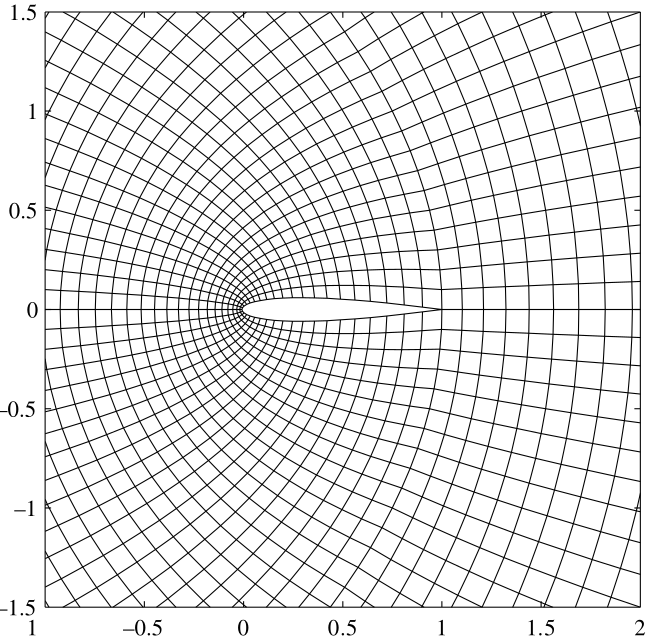
\includegraphics[width=.55\textwidth]{airfoil}
\caption{Rendering of an \textit{airfoil} mesh. Diagram from \cite{gpudesign}}
\label{fig:airfoil_mesh}
\end{figure}
\par
\vfill
\noindent To ensure that the test cases selected definitely validate the implementation, the requirements set out in the Specification must be revisited. They are summarised in the next Section.
\clearpage
\subsection{Requirements}
  \begin{outline}[enumerate]
  \1 Source code files must be produced as the output of the new code generation Python script.
  \1 The generated source code files must be valid.
  \2 C code must compile using \verb|icc| without errors;
  \2 CUDA code must compile with \verb|nvcc| without errors.
  \1 The compiled executable must invoke a re-compilation stage, if the feature is enabled.
  \2 Re-compilation must also complete without error;
  \2 The binary must execute code that has been compiled during its execution.
  \1 Constant values from the input must be available to the User Function.
  \2 If JIT is enabled, they must be turned into \verb|#define| directives;
  \2 Otherwise they must be copied to device memory.
  \1 The compiled executable must produce a result within some tolerance of the expected result.
  \1 The OP2 API must not be modified.
  \end{outline}

\noindent Section \ref{ss:results} is the final results of the test plan used throughout the project whenever a work done needed to be validated. Each test  ensures that a requirement from the above list has been met, and also includes the date when it first passed.
\par
Requirement 6 can be trivially accepted when testing, since the implementation did not modify the OP2 API. There is no test for this requirement.

\subsection{Initial State}
\begin{wrapfigure}[18]{l}{0.45\textwidth}
  \centering
\caption{\textit{airfoil} folder initial state}
\label{fig:files_a}
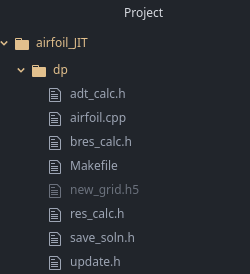
\includegraphics[width=0.4\textwidth]{files1}
\end{wrapfigure}
The initial state for testing is a folder containing the source files for \textit{airfoil}, as listed in Figure \ref{fig:files_a}. The Application File is \verb|airfoil.cpp|, and the five header files each contain a User Function for the parallel loop with the same name.
\par
\verb|new_grid.h5| is the name of the input data file, formatted in the Heterogeneous Data Format (HDF5) \cite{HDF5}. This file can be obtained from the OP2 website \cite{op-dsl}, and must be converted from \verb|.txt| to \verb|.h5| using the \verb|convert_mesh| tool.
\par
OP2 already provides a standard set of functions for performing file I/O on an HDF5 file, which \textit{airfoil} uses. The contents of the file can be viewed using the \verb|hdump| utility, which comes with an HDF5 installation.

\clearpage
\subsection{Test Plan \& Results}
\label{ss:results}

\hspace{\parindent}\minititle{``Source code files must be produced as the output of the new code generation Python script."}
To test the code generation, the python script \verb|op2.py| is called in the directory, passing the main application file \verb|airfoil.cpp| as an argument, as well as the string \verb|JIT| to make sure the correct GPU code generation script is used. \par
The environmental variable \verb|$OP2_INSTALL_PATH| can be assumed to hold to full path to the \verb|op2/| folder in the top level of the OP2 repository. Since the translation script is in a sub-directory of \verb|translator/|, which is also a top-level folder, the path to the Python translator script will be as shown below.
\codeline{> python2 \$OP2_INSTALL_PATH/../translator/c/python/op2.py airfoil.cpp JIT}{}

\noindent After running this command in the \textit{airfoil} directory, the expected outcome is that a new file: \verb|airfoil_op.cpp| is created, as well as a new directory named \verb|cuda/|, which will contain with eleven CUDA source code files it: two kernel files for each of the five parallel loops, and a single Central Kernels File, named \verb|airfoil_kernels.cu|.
\par
This test is considered a pass if these files exist, as their contents will be validated as correct if the following tests pass. A folder called \verb|seq/| is also created by the translator script \verb|translator/c/python/jit/op2_gen_seq_jit.py|, which was not completed as part of this project, but part of the \verb|feature/lazy-execution| branch.
\par
If the environmental variable \verb|OP_AUTO_SOA| is set to one, the code will be generated with transformations to automatically use the Struct-of-Arrays data structures, overwriting any generated source files that exist already. To confirm the functionality is working with both, the generated files need to be deleted, and the script invoked again once the environmental variable has been set.

\begin{wrapfigure}[13]{l}{0.45\textwidth}
\caption{\textit{airfoil} folder after Code Generation}
\label{fig:files_b}
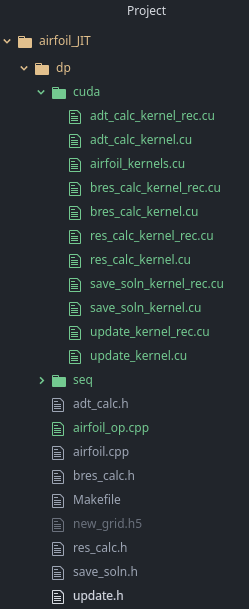
\includegraphics[width=0.4\textwidth]{files2}
\end{wrapfigure}
\par
Figure \ref{fig:files_b} shows the folder after a passing test case of running the OP2 translation script. The folder appears identical whether automatic\\ Struct-of-Arrays transformation is enabled or not, which is the expected outcome, so the Figure has not been duplicated.\par
When compared to Figure \ref{fig:files_a}, all the additional files have been generated by the code generation script. As expected, there are two kernel files for each parallel loop, and a single Central Kernels File in the \verb|cuda/| directory, and a Modified Application file in the root.
\par

\testresult{pass}{03/12/2019}

\minititle{``The generated source code files must be valid."}
The validity of the generated source code files will be confirmed by the initial compilation of the binary completing without error, both when JIT compilation is enabled and disabled. Recall that even with JIT compilation enabled, the AOT compiler is still required to produce an initial binary. If any errors are produced by the compiler, the code generated is not valid, and therefore is of no further use.
\par
In the \verb|airfoil_JIT| folder, compilation is done using the Makefile, and for the initial compilation of the binary, the target is \verb|airfoil_cuda|. The Makefile produces a binary with JIT compilation enabled by default, so the command to compile it will be: \\\verb|make airfoil_cuda|
\par Whereas, to produce a binary that will execute only Ahead-Of-Time compiled code, the command will be: \\\verb|make airfoil_cuda JIT=FALSE|
\par \noindent The resulting command executed by the Makefile is: \vspace{-1em}
\begin{verbatim}
nvcc -gencode arch=compute_60,code=sm_60 -m64 -Xptxas=-v
   --use_fast_math -O3 -lineinfo [-DOP2_JIT]
   -I$OP2_INSTALL_PATH/c/include
   -I$HDF5_INSTALL_PATH/include -Icuda -I.
   -c -o cuda/airfoil_kernels_cu.o cuda/airfoil_kernels.cu
\end{verbatim}
The inclusion of \verb|-DOP2_JIT| depends on which of the two above commands was called. Both commands will need to be tested for errors when the code base has been generated both with and without automatic Struct-of-Arrays transformations, giving four test cases. The generated code will also need to be manually inspected to ensure that transformations have been made when \verb|OP_AUTO_SOA| is enabled.
\begin{wrapfigure}[18]{l}{0.45\textwidth}
\caption{\textit{airfoil} folder after Ahead-Of-Time compilation}
\label{fig:files_c}
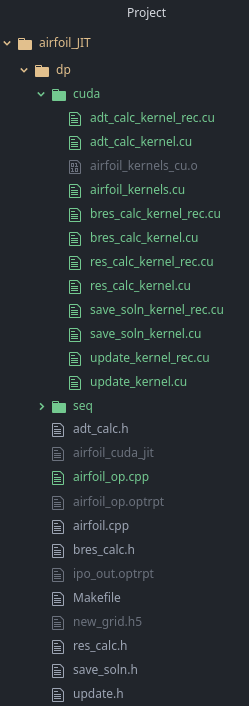
\includegraphics[width=0.4\textwidth]{files3}
\end{wrapfigure}
\par
\noindent Figure \ref{fig:files_c} shows the folder after the make command has been successfully executed. As before, the folder will appear almost identical for all four test cases, so the Figure has not been duplicated.\par
In the figure the first new file that can be seen is a single object file in the \verb|cuda/| folder, which is the result of compiling the Central Kernels File and all the kernels that are not marked \verb|_rec| into a single object binary.
\par  In the parent directory the executable \verb|airfoil_cuda_jit| has been generated, which statically links the above object file, so does not require access to it at run-time. If JIT compilation is not enabled, the binary is just called \verb|airfoil_cuda|.\par Lastly, a number of optimisation reports have been generated by the Intel C compiler.\par
\vspace{3cm}
\noindent The test results and dates for the four test cases are shown in a matrix below.
\begin{table}[h]
\centering
\renewcommand{\arraystretch}{1.5}
\begin{tabular}{| c || c | c |}
\hline
JIT & \verb|OP_AUTO_SOA=0| & \verb|OP_AUTO_SOA=1| \\
\hhline{|=|=|=|}
TRUE &\textbf{\textcolor{green!20!black}{PASSED}}. 16/01/2020 &\textbf{\textcolor{green!20!black}{PASSED}}. 17/01/2020 \\
\hline
FALSE&\textbf{\textcolor{green!20!black}{PASSED}}. 16/01/2020 &\textbf{\textcolor{green!20!black}{PASSED}}. 17/01/2020 \\
\hline
\end{tabular}
\end{table}

\minititle{``The compiled executable must invoke a re-compilation stage, if the feature is enabled."}
\label{sss:jit_comp}
For this test to be considered a pass, a compiler process must be started during the execution of the binary, and must complete without producing errors. As described previously, in Section \ref{sss:mkf}, there exists a check for success in the code, and the terminal output of the compilation is dumped to a file named \verb|jit_compile.log|.
\par
The executable printing the compilation duration to the console output like the example below confirms the compilation has completed, and success can be confirmed by checking the compiler log for errors. If none are found, requirement \textbf{3i} has been met: \textbf{``Re-compilation must also complete without error"}.

\begin{figure}[h!]
  \caption{\label{fig:jit_ex}Example success output}
\begin{verbatim}
> ./airfoil_cuda_jit
...
JIT compiling op_par_loops
  Completed: 5.588549s
\end{verbatim}
\end{figure}

\par\noindent
It should be the case that these lines are \textbf{not} printed if the executable was compiled with JIT compilation disabled, otherwise the part of the requirement that states \textbf{``\ldots, if the feature is enabled"} has been violated.\par
In order to determine whether sub-requirement \textbf{3ii} has been met: \textbf{``The binary must execute code that has been compiled during its execution"}, one of the Kernel files that will be compiled at runtime is manually edited to contain a print statement, or some other identifier to confirm which version is being executed: the run-time compiled or the original.\par
As with the second requirement there are 4 test cases. It is possible that the state of \verb|OP_AUTO_SOA| could interfere, so both enabled and disabled will need to be tested for both possible states for JIT compilation.
\clearpage
\begin{wrapfigure}[21]{l}{0.45\textwidth}
\caption{\textit{airfoil} folder after Just-In-Time Compilation}
\label{fig:files_d}
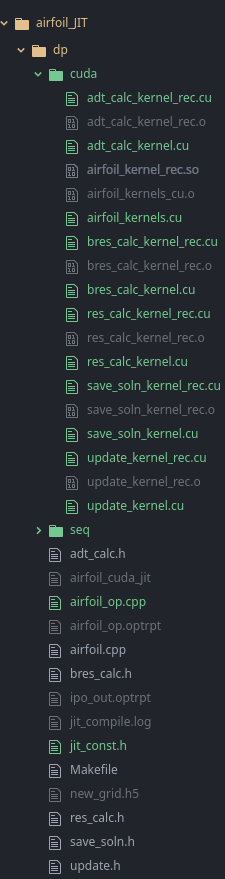
\includegraphics[width=0.4\textwidth]{files4}
\end{wrapfigure}
Figure \ref{fig:files_d} shows the \textit{airfoil} folder after the JIT compilation stage has completed successfully. In the Figure, there is now an object file for each of the parallel loops, as well as a new shared object in the \verb|cuda/| folder, which will have been loaded by the running executable. Some other files have also been generated, including the compilation log file \verb|jit_compile.log|, and the constants header file \verb|jit_const.h| which is part of the next requirement.
\par
The JIT compilation log file does not contain any errors, and the expected files have been generated, so the main part of the requirement has been met.
\par
Manually adding a print statement to only the re-compiled kernels confirms that the correct kernels are being executed, and JIT compilation is enabled, the executable is utilising functions that have been compiled as part of it's execution.
\begin{table}[b]
\raggedleft
\renewcommand{\arraystretch}{2.5}
\begin{tabular}{| c || c | c |}
\hline
JIT & \verb|OP_AUTO_SOA=0| & \verb|OP_AUTO_SOA=1| \\
\hhline{|=|=|=|}
TRUE & \shortstack{\textbf{\textcolor{green!20!black}{PASSED}}.\\22/01/2020} &\shortstack{\textbf{\textcolor{green!20!black}{PASSED}}.\\22/01/2020} \\
\hline
FALSE&\shortstack{\textbf{\textcolor{green!20!black}{PASSED}}.\\22/01/2020} &\shortstack{\textbf{\textcolor{green!20!black}{PASSED}}.\\22/01/2020} \\
\hline
\end{tabular}
\hspace{-0.5cm}
\end{table}

\minititle{``Constant values from the input must be available to the User Function."}
This test simply requires that the User Function is able to access the values of input constants when they are executing on the GPU. For Kernels compiled with JIT compilation disabled, this requires that they are copied to device memory, and for JIT enabled Kernels they must be defined literals.
\par
The \textit{airfoil} program includes a number of input constants, where six have a dimension of 1, and one has a dimension of 4 named \verb|qinf| - all holding values of the type \verb|double|. It never exercises the functionality of accessing \verb|qinf| using an expression however, so to test that this functionality works correctly, additional code needs to be added inside the User Function.
\par This can be solved at the same time as testing the other constants by adding to the code generation script, such that inside the User Function the values of constants are printed. This should include a loop over \verb|qinf| such that it is accessed using an index variable, and with literal values.

\begin{lstlisting}[backgroundcolor=\color{lightgray!20}, language=Python]
|IF('blockIdx.x == 0 && threadIdx.x == 0')
|for nc in range (0,len(consts)):
|  comm(consts[nc]['name'])
|  if consts[nc]['dim']==1:
|  code('printf("'+name+'-'+consts[nc]['name']+
        ': %1.17e\\n",'+ consts[nc]['name']+');')
|  else:
|    FOR('i','0',consts[nc]['dim'])
|    code('printf("'+name+'-'+consts[nc]['name']+
          '[%d]: %1.17e\\n", i,'+consts[nc]['name']+'[i]);')
|    ENDFOR()
|    for i in range (0,int(consts[nc]['dim'])):
|      code('printf("'+name+'-'+consts[nc]['name']+
            '['+str(i)+']: %1.17e\\n",'+ consts[nc]['name']+
            '['+str(i)+']);')
|ENDIF()
\end{lstlisting}
The above code is left in the translator script, at lines [259-281], but has been commented out as printing this much to the terminal is very detrimental to performance. It should not be included for benchmarking or production code generation.
\par
For \textit{airfoil}, the code added to the end of the JIT enabled \verb|save_soln| User Function is:
\begin{lstlisting}[backgroundcolor=\color{red!20},language=C]
|  if (blockIdx.x == 0 && threadIdx.x == 0) {
|    //gam
|    printf("save_soln-gam: %1.17e\n",gam);
|    //gm1
|    printf("save_soln-gm1: %1.17e\n",gm1);
|    //cfl
|    printf("save_soln-cfl: %1.17e\n",cfl);
|    //eps
|    printf("save_soln-eps: %1.17e\n",eps);
|    //mach
|    printf("save_soln-mach: %1.17e\n",mach);
|    //alpha
|    printf("save_soln-alpha: %1.17e\n",alpha);
|    //qinf
|    for (int i = 0; i < 4; ++i)
|    {
|      printf("save_soln-qinf_OP2CONSTANT[%d]: %1.17e\n", i,
               qinf_OP2CONSTANT[i]);
|    }
|    printf("save_soln-qinf_0_OP2CONSTANT: %1.17e\n",
             qinf_0_OP2CONSTANT);
|    printf("save_soln-qinf_1_OP2CONSTANT: %1.17e\n",
             qinf_1_OP2CONSTANT);
|    printf("save_soln-qinf_2_OP2CONSTANT: %1.17e\n",
             qinf_2_OP2CONSTANT);
|    printf("save_soln-qinf_3_OP2CONSTANT: %1.17e\n",
             qinf_3_OP2CONSTANT);
|  }
\end{lstlisting}
When the above lines are included, the expected output for each loop is that each one dimensional constant will be printed along with the function it is being used in. Then, the multi value constants will be printed twice: once using a variable \verb|i| to index it, and again using literal values.
\par
The generated code for an AOT kernel is similar, but with modified references to the constants, since constant references are managed using a string replacement on all places where they appear in the User Function.\par
\clearpage
\noindent When the \verb|save_soln| loop is executed, the terminal output with JIT compilation is enabled will be the following if the values are available and correct:
\begin{lstlisting}[frame=none]
save_soln-gam: 1.39999997615814209e+00
save_soln-gm1: 3.99999976158142090e-01
save_soln-cfl: 8.99999976158142090e-01
save_soln-eps: 5.00000007450580597e-02
save_soln-mach: 4.00000005960464478e-01
save_soln-alpha: 5.23598775598298830e-02
save_soln-qinf_OP2CONSTANT[0]: 1.00000000000000000e+00
save_soln-qinf_OP2CONSTANT[1]: 4.73286385670476317e-01
save_soln-qinf_OP2CONSTANT[2]: 0.00000000000000000e+00
save_soln-qinf_OP2CONSTANT[3]: 2.61200015044213218e+00
save_soln-qinf_0_OP2CONSTANT: 1.00000000000000000e+00
save_soln-qinf_1_OP2CONSTANT: 4.73286385670476317e-01
save_soln-qinf_2_OP2CONSTANT: 0.00000000000000000e+00
save_soln-qinf_3_OP2CONSTANT: 2.61200015044213218e+00
\end{lstlisting}

\noindent Furthermore, when an \textit{airfoil} binary with JIT compilation enabled is executed, the \verb|jit_const.h| file should contain the following statements. Values correspond with those above.
\begin{lstlisting}[backgroundcolor=\color{green!20}, language=C]
|#define gam 1.39999997615814209e+00
|#define gm1 3.99999976158142090e-01
|#define cfl 8.99999976158142090e-01
|#define eps 5.00000007450580597e-02
|#define mach 4.00000005960464478e-01
|#define alpha 5.23598775598298830e-02
|#define qinf_0_OP2CONSTANT 1.00000000000000000e+00
|#define qinf_1_OP2CONSTANT 4.73286385670476317e-01
|#define qinf_2_OP2CONSTANT 0.00000000000000000e+00
|#define qinf_3_OP2CONSTANT 2.61200015044213218e+00
\end{lstlisting}
\vfill
\noindent The test results and dates for the four test cases are shown in a matrix below.
\begin{table}[h]
\centering
\renewcommand{\arraystretch}{1.5}
\begin{tabular}{| c || c | c |}
\hline
JIT & \verb|OP_AUTO_SOA=0| & \verb|OP_AUTO_SOA=1| \\
\hhline{|=|=|=|}
TRUE &\textbf{\textcolor{green!20!black}{PASSED}}. 21/01/2020 &\textbf{\textcolor{green!20!black}{PASSED}}. 21/01/2020 \\
\hline
FALSE&\textbf{\textcolor{green!20!black}{PASSED}}. 21/01/2020 &\textbf{\textcolor{green!20!black}{PASSED}}. 21/01/2020 \\
\hline
\end{tabular}
\end{table}
\clearpage
\minititle{``The compiled executable must produce a result within some tolerance of the expected result."}
The final test is that the result of the execution is within tolerance of the expected result. This test confirms that the contents of the file are not just valid but also correct.

\tinytitle{Expected Result}
The \textit{airfoil} OP2 application prints the value of the \verb|rms| (root mean square) variable every 100 iterations. According to the documentation, the first 1000 iterations for double precision should be exactly:\\
\begin{table}[h!]
\vspace{-2em}
\centering
\renewcommand{\arraystretch}{1.2}
\begin{tabular}{c c || c }
& & \verb|rms| \\
\hline
\multirow{10}{*}{Iterations} & 100 & $ 5.02186\times10^{-4} $ \\
& 200 & $ 3.41746\times10^{-4} $ \\
& 300 & $ 2.63430\times10^{-4} $ \\
& 400 & $ 2.16288\times10^{-4} $ \\
& 500 & $ 1.84659\times10^{-4} $ \\
& 600 & $ 1.60866\times10^{-4} $ \\
& 700 & $ 1.42253\times10^{-4} $ \\
& 800 & $ 1.27627\times10^{-4} $ \\
& 900 & $ 1.15810\times10^{-4} $ \\
& 1000 & $ 1.06011\times10^{-4} $
\end{tabular}
\caption{Expected values of rms}
\label{tab:expected}

\end{table}

\noindent The application code also includes a test of the result after 1000 iterations, which compares against the expected outcome and prints the calculated percentage difference using the equation:
\[\%diff = \abs{ (100 \times \frac{rms}{0.0001060114637578}) - 100 }\]
A difference of less than 0.00001\% is considered within tolerance due to the potential for minor floating point errors.
\clearpage
\tinytitle{Actual Results}

\noindent The tables below show the results output by the compiled binary every 100 iterations.
\begin{table}[H]
\renewcommand{\arraystretch}{1.2}
\caption{Console Output when JIT compilation is Enabled}
\label{tab:output}
\begin{tabular}{c c || c | c }
&  & \verb|OP_AUTO_SOA=0| & \verb|OP_AUTO_SOA=1| \\
\hline
\multirow{10}{*}{Iterations} & 100  & $ 5.02186\times10^{-4} $ & $ 5.02186\times10^{-4} $  \\
& 200  & $ 3.41746\times10^{-4} $ & $ 3.41746\times10^{-4} $  \\
& 300  & $ 2.63430\times10^{-4} $ & $ 2.63430\times10^{-4} $  \\
& 400  & $ 2.16288\times10^{-4} $ & $ 2.16288\times10^{-4} $  \\
& 500  & $ 1.84659\times10^{-4} $ & $ 1.84659\times10^{-4} $  \\
& 600  & $ 1.60866\times10^{-4} $ & $ 1.60866\times10^{-4} $  \\
& 700  & $ 1.42253\times10^{-4} $ & $ 1.42253\times10^{-4} $  \\
& 800  & $ 1.27627\times10^{-4} $ & $ 1.27627\times10^{-4} $  \\
& 900  & $ 1.15810\times10^{-4} $ & $ 1.15810\times10^{-4} $  \\
& 1000  & $ 1.06011\times10^{-4} $ & $ 1.06011\times10^{-4} $  \\
\hline
&&&\\
Accuracy & & $2.484679129111100\times10^{-11} \%$ & $2.489120021209601\times10^{-11} \%$ \\
&&&\\
\hline
\end{tabular}
\newline
\newline
\caption{Console Output when JIT compilation is Disabled}
\label{tab:output}
\begin{tabular}{c c || c | c }
&  & \verb|OP_AUTO_SOA=0| & \verb|OP_AUTO_SOA=1| \\
\hline
\multirow{10}{*}{Iterations} & 100  & $ 5.02186\times10^{-4} $ & $ 5.02186\times10^{-4} $  \\
& 200  & $ 3.41746\times10^{-4} $ & $ 3.41746\times10^{-4} $  \\
& 300  & $ 2.63430\times10^{-4} $ & $ 2.63430\times10^{-4} $  \\
& 400  & $ 2.16288\times10^{-4} $ & $ 2.16288\times10^{-4} $  \\
& 500  & $ 1.84659\times10^{-4} $ & $ 1.84659\times10^{-4} $  \\
& 600  & $ 1.60866\times10^{-4} $ & $ 1.60866\times10^{-4} $  \\
& 700  & $ 1.42253\times10^{-4} $ & $ 1.42253\times10^{-4} $  \\
& 800  & $ 1.27627\times10^{-4} $ & $ 1.27627\times10^{-4} $  \\
& 900  & $ 1.15810\times10^{-4} $ & $ 1.15810\times10^{-4} $  \\
& 1000  & $ 1.06011\times10^{-4} $ & $ 1.06011\times10^{-4} $  \\
\hline
&&&\\
Accuracy & & $2.486899575160351\times10^{-11} \%$ & $2.493560913308102\times10^{-11} \%$ \\
&&&\\
\hline
\end{tabular}
\end{table}
\vspace{-1.5em}
\noindent All of these results are well within tolerance. The requirement has been met.

\subsection{Benchmarking}
The functionality has now been confirmed to work as intended, and the technical requirements of the project have all been met: new code is able to be generated by the OP2 translator script, which can be compiled into a binary that will execute code it has compiled itself as part of it's execution. What remains is to benchmark the run-time of the application with JIT compilation enabled and disabled, and determine if there is any performance gain.
\par
The following results should be considered a benchmark of the Constant Definition optimisation, rather than JIT compilation as a whole, as further assertions at run-time are possible and could make even more use of the compiler being aware of the input data.

\subsubsection{Hardware}
Testing was done on a personal computer with an NVIDIA GeForce MX250 Graphics Card \cite{mx250} - and while this is able to execute the CUDA code and ensure it produces the right output, it is not sufficient to gather representative benchmarking data for the runtime of the \textit{airfoil} application. Using a personal computer system may result in noisy data, for example from the Operating System scheduling other tasks.
\par
In order to gather better data, access to a HPC cluster located in Cambridge, part of the Cambridge Service for Data-Driven Discovery (CSD3) \cite{csd3}, was approved - with the caveat that workloads for this project would be placed in a low priority queue.
\par
The supercomputer named \textit{Wilkes2} was used, which is the largest GPU enabled supercomputer for academic research in the UK. \textit{Wilkes2} has 90 nodes, each with the specifications in Table \ref{tab:wilkes2} \cite{wilkes2}. \clearpage

\begin{table}[h]
  \centering
  \renewcommand{\arraystretch}{1.5}
  \caption{\textit{Wilkes2} hardware specification}
  \label{tab:wilkes2}
\begin{tabular}{c |r l c}
CPU & 1 x&12-core Intel Xeon E5-2650 v4 2.2GHz & \cite{xeon}\\
RAM & &96GB &\\
GPU & 4 x&NVidia P100 16GB &\cite{p100}\\
\end{tabular}
\end{table}

\noindent The translator currently only generates code for a single graphics card, so only one of the four will be used. A possible extension would be to include MPI and divide the workload across multiple GPUs.

\subsubsection{Benchmarking Strategy}
The \textit{airfoil} program was also used for benchmarking, as it is reasonably representative of production applications. The input mesh remains the same size as in the previous Section where it was used for testing functionality, with 721,801 nodes, but the number of time step iterations was upped from 1000 to 1,000,000 to make any differences in run-time more noticeable. OP2's internal timing functions are used to sum the total time spent in each of the parallel loops, which can be compared between the versions with JIT compilation enabled and disabled.
\par
As discussed in Section \ref{sss:jit_comp} (Just-In-Time Compilation), the time taken for the invocation of the compiler at run-time to complete is also recorded, and will be included in the data. It is a one-time cost at the start of execution, but still needs to be considered.
% \par
% Given more time other OP2 applications would also have been used to compare data, however, finding a suitable HPC system and gaining access took a larger portion of the project's duration than expected.
\clearpage
\subsubsection{Results}
The graph in Figure \ref{fig:res_total} shows the mean total run-time of the four different configurations, averaged from five executions, in an attempt to further reduce any noise from factors other than those being tested. The percentage speed-up from the original version (blue) to JIT compiled (green) is shown above each pair of bars.

\begin{figure}[h!]
\begin{center}
\caption{Total Execution Time}
\label{fig:res_total}
\pgfplotsset{width=.6\linewidth,compat=1.8}
\begin{tikzpicture}
\begin{axis}[
  ybar,
  ymin=1000,
  ymax=2500,
  bar width=.6cm,
  enlargelimits=0.05,
  enlarge x limits={abs{0.5}},
  legend style={at={(1,0.95)},
    anchor=north},
  ylabel={Execution Time/s},
  symbolic x coords={Total},
  xtick=data,
  nodes near coords={},
  every node near coord/.append style={yshift=5pt}
  ]
  \addplot+[blue, fill=blue!20, name nodes near coords=AOTAOS]
  coordinates {(Total,2379.0361)};
  \addplot+[green!50!black,fill=green!20, name nodes near coords=JITAOS]
  coordinates {(Total,2378.349309)};
  \addplot+[blue, pattern=custom north west lines, hatchspread=1em, hatchcolor=blue!20, name nodes near coords=AOTSOA]
  coordinates {(Total,1910.25154)};
  \addplot+[green!50!black, pattern=custom north west lines, hatchspread=1em, hatchcolor=green!60, name nodes near coords=JITSOA]
  coordinates {(Total,1912.105723)};
\legend{JIT Disabled AoS,JIT Enabled AoS,JIT Disabled SoA,JIT Enabled SoA}
\end{axis}
\path (AOTAOS0) -- (JITAOS0) node[midway] (A) {0.03\%};
\path (AOTSOA0) -- (JITSOA0) node[midway] (A) {-0.1\%};
\end{tikzpicture}
\end{center}
\vspace{-1cm}
\end{figure}

\noindent The speed-up percentages above the bars were calculated using the formula below:
\[ \%speedup = \frac{\text{Initial Time}-\text{New Time}}{\text{Initial Time}} \times 100\%\]
Therefore a positive value indicates that the JIT compiled version completed faster, while a negative value indicates it was outperformed by the original.

\tinytitle{Analysis}

\noindent In Figure \ref{fig:res_total}, the speed-up for Array-of-Structs data layout is 0.03\%, which is only a very small improvement coming to about 1 second saved out of nearly 40 minutes. However the setup cost of run-time compilation is an average of 4.13 seconds, compared to essentially zero seconds to copy constants to device memory (0.0001s for all \textit{airfoil} constants). This duration does not vary significantly when either the size of the mesh or the number of iterations is increased.
\par
If the re-compilation time is excluded, the speed-up is 0.2\% for the actual execution of the application. From this, and the fact that compilation time is O(1) for input size, it follows that the speed-up could increase linearly with problem size, albeit at a shallow gradient. There will always be a constant initial cost, but every single iteration will complete fractionally faster. More iterations means more time saved.
\par
Unfortunately, when \verb|OP_AUTO_SOA=1| the object difference is that the executable with JIT compilation enabled is 0.1\% slower. As before, it should be considered that JIT compilation incurs a larger one-time cost at the start, and comparing just the application execution the runtime is 0.14\% faster. It would seem there is benefit possible for the SOA enabled build, but the problem size needs to be even greater for the per-iteration time reduction to outweigh the upfront cost, and the total execution time to be reduced.\par
\subsubsection{Results by Parallel Loop}
The runtime can be broken down into how long the application spent executing each of the parallel loops, and what speed-up each loop was able to see when applying JIT compilation. In the chart on the next page (Figure \ref{fig:res_func}), the speed-up of each parallel loop is plotted. Once again, a percentage is given above each pair of bars, which is the speed-up of the JIT compiled version compared to the version with JIT compilation disabled.
\par
As in Figure \ref{fig:res_total}, a positive value indicates that the JIT compilation enabled version completed faster, while a negative percentage means the version without JIT compilation had the shorter runtime.
\clearpage
\begin{figure}[ht]
\begin{center}
\caption{Execution Time by Function}
\label{fig:res_func}

\pgfplotsset{width=1.1\linewidth,compat=1.8}
\makebox[\textwidth][c]{
\begin{tikzpicture}
\begin{axis}[
  ybar,
  bar width=.5cm,
  enlargelimits=0.01,
  ymin=0,
  ymax=1400,
  enlarge x limits={abs{0.1}},
  legend style={at={(.05,.95)},
    anchor=north west},
  ylabel={Execution Time/s},
  symbolic x coords={setup,save\_soln,adt\_calc,res\_calc,bres\_calc,update},
  xtick=data,
  x tick label style={rotate=45,anchor=east},
  nodes near coords={},
  every node near coord/.append style={yshift=5pt}
  ]
  \addplot+[blue, fill=blue!20, name nodes near coords=AOTAOS]
  coordinates
  {(setup,0) (save\_soln,149.6223833) (adt\_calc,242.9445833) (res\_calc,1324.230383) (bres\_calc,25.66483333) (update,636.5739167)};
  \addplot+[green!50!black,fill=green!20, name nodes near coords=JITAOS]
  coordinates
  {(setup,4.125742667) (save\_soln,148.9582667) (adt\_calc,240.1570667) (res\_calc,1324.5283) (bres\_calc,25.20193333) (update,635.378)};
  \addplot+[blue, pattern=custom north west lines, hatchspread=1em, hatchcolor=blue!20, name nodes near coords=AOTSOA]
  coordinates
  {(setup,0) (save\_soln,99.07338) (adt\_calc,239.80552) (res\_calc,1028.33054) (bres\_calc,29.6906) (update,513.3515)};
  \addplot+[green!50!black, pattern=custom north west lines, hatchspread=1em, hatchcolor=green!60, name nodes near coords=JITSOA]
  coordinates
  {(setup,3.993373) (save\_soln,98.793325) (adt\_calc,238.07195) (res\_calc,1027.164025) (bres\_calc,29.023825) (update,515.059225)};

\legend{JIT Disabled AoS,JIT Enabled AoS,JIT Disabled SoA,JIT Enabled SoA}
\end{axis}
\path (AOTAOS0) -- (JITAOS0) node[midway] (A) {\small N/A};
\path (AOTSOA0) -- (JITSOA0) node[midway] (A) {\small N/A};

\path (AOTAOS1) -- (JITAOS1) node[midway] (A) {\small 0.44\%};
\path (AOTSOA1) -- (JITSOA1) node[midway] (A) {\small 0.28\%};

\path (AOTAOS2) -- (JITAOS2) node[midway] (A) {\small 1.15\%};
\path (AOTSOA2) -- (JITSOA2) node[midway] (A) {\small 0.72\%};

\path (AOTAOS3) -- (JITAOS3) node[midway] (A) {\small -0.02\%};
\path (AOTSOA3) -- (JITSOA3) node[midway] (A) {\small 0.11\%};

\path (AOTAOS4) -- (JITAOS4) node[midway] (A) {\small 1.80\%};
\path (AOTSOA4) -- (JITSOA4) node[midway] (A) {\small 2.25\%};

\path (AOTAOS5) -- (JITAOS5) node[midway] (A) {\small 0.19\%};
\path (AOTSOA5) -- (JITSOA5) node[midway] (A) {\small -0.33\%};
\end{tikzpicture}
}
\end{center}
\end{figure}
\vspace{-1cm}
\noindent The speed-up of the setup stage is marked Not Applicable (instead of negative four million percent) since the time taken to copy constants to device memory for \textit{airfoil} is essentially zero seconds.

\tinytitle{Analysis}

\noindent As with most HPC applications, different loops in \textit{airfoil} take up different proportions of the runtime. In Figure \ref{fig:res_func} it is clear that \textit{res\_calc} dominates the runtime, and is also the least able to benefit from the Constant Definition optimisation made in the JIT compiled code, since it was actually marginally slower for AoS. Looking into the source code, the loop body only uses the input constants three times: \verb|gm1| twice in quick succession, so would likely still be cached in the AOT compiled version; then \verb|eps| once a few lines later.
\par
Comparing this to \textit{bres\_calc}, which was the best affected by Constant Definition, the pattern holds as this function makes sixteen references to \verb|qinf|, as well as using \verb|gm1| twice. Although this could not be tested in the time available, it would seem logical that if the function that dominates the runtime is also making heavy use of input constants, the overall benefit to the application could be greater.
\par
\subsubsection{Results Conclusion}
What the results demonstrate most of all, is that there is definitely potential in Just in Time compilation. At one million time steps, the optimisation of Constant Definition was able to approximately make up the cost of re-compilation through fractional reduction in the time taken to perform every iteration, and increasing the problem size would only improve the speed-up.
\par
Since the assertion being made is only that values declared constant will remain constant, the time available for optimisation is only the time taken to read constant values from memory, which will not usually make up a significant proportion of the run-time.
\par
If more optimisations are implemented, which make further use of the inputs being known, and the per-iteration speed-up is increased, then the required problem size to see benefit will shrink, and the technique becomes even more valuable.
\par
Even without further optimisations, a small improvement to a very large solver application, which might be executing many millions of time-step iterations, can quickly outweigh the relatively tiny one-time cost of recompilation, and start to make an improvement to the overall runtime.

% !TEX root =  ../report.tex
% !TeX spellcheck = en-GB

\section{Evaluation}
\label{s:eval}

This project was intended as an investigation, and therefore it can certainly be considered successful. The potential for optimisation through JIT compilation has been proved, via the demonstration that the optimisation of defining constants as literal values is able to re-coup the cost of run-time compilation, if the problem size is sufficiently large.
\par
Since the space for optimisation by this technique is relatively small, the problem size does have to be very large to see benefit. However HPC applications do tend to be very large, hence why they are not run on normal computers. This is not a significant restriction.
\par
It is very promising that this optimisation is able to provide any benefit at all, and as a result of the contributions made to the OP2 Framework while completing this project, important groundwork has been laid for future contributors to build on top of. Further optimisations and run-time assertions can be implemented as extensions to this implementation, which might achieve greater speedup at run-time, especially for smaller problem sizes.

\subsection{Future Work}
\label{ss:fw}

\subsubsection{Run-Time Assertions}
As previously mentioned, it seems necessary for more assertions to be made at run-time in order to produce more effective speed-up after JIT compilation. \par
There are a number of possible loop optimisations which could be made, including identifying a loop inside a kernel, and at run-time having the loop bound be hard-coded to remove the need to evaluate the expression of every iteration.
\par Another possible optimisation would be Loop Fusion where two separate parallel loops might be provably able to be fused into a single loop, but only if the inputs allow for it - meaning this could only be done at run-time.

\noindent There is also current research into automatically applying loop tiling to the generated code, which is dividing the iterations of a loop into sub-regions where both temporal and spatial locality in memory can be exploited. \par

\begin{wrapfigure}{r}{.4\textwidth}
  \centering
  \caption{2D Loop Tiling}
  \label{fig:tile2D}
  \hspace{-1em}
  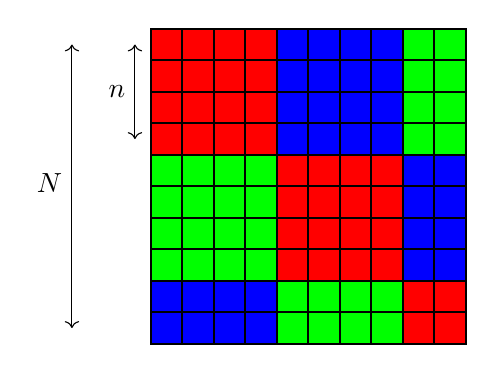
\begin{tikzpicture}
      [%%%%%%%%%%%%%%%%%%%%%%%%%%%%%%
          box/.style={rectangle,draw=black,thick, minimum size=.4cm},
          scale=0.4
      ]%%%%%%%%%%%%%%%%%%%%%%%%%%%%%%

  \foreach \x in {0,...,9}{
      \foreach \y in {0,...,9}
          \node[box] at (\x,\y){};
  }

  \foreach \x in {0,...,3}{
      \foreach \y in {6,...,9}
        \node[box,fill=red] at (\x,\y){};
  }

  \foreach \x in {4,...,7}{
      \foreach \y in {6,...,9}
        \node[box,fill=blue] at (\x,\y){};
  }

  \foreach \x in {8,...,9}{
      \foreach \y in {6,...,9}
        \node[box,fill=green] at (\x,\y){};
  }

  \foreach \x in {0,...,3}{
      \foreach \y in {2,...,5}
        \node[box,fill=green] at (\x,\y){};
  }

  \foreach \x in {4,...,7}{
      \foreach \y in {2,...,5}
        \node[box,fill=red] at (\x,\y){};
  }

  \foreach \x in {8,...,9}{
      \foreach \y in {2,...,5}
        \node[box,fill=blue] at (\x,\y){};
  }

  \foreach \x in {0,...,3}{
      \foreach \y in {0,...,1}
        \node[box,fill=blue] at (\x,\y){};
  }

  \foreach \x in {4,...,7}{
      \foreach \y in {0,...,1}
        \node[box,fill=green] at (\x,\y){};
  }

  \foreach \x in {8,...,9}{
      \foreach \y in {0,...,1}
        \node[box,fill=red] at (\x,\y){};
  }

  \draw[<->] (-1,6) -- (-1,9);
  \node[anchor=south east] at (-1,7) {$n$};
  \draw[<->] (-3,0) -- (-3,9);
  \node[anchor=south east] at (-3,4) {$N$};

  \end{tikzpicture}
\end{wrapfigure}
For example, a loop iterating over a 2D array of size $N \times N$, with Level 1 (L1) cache size of $n$, such that $n < N$, would benefit from dividing the array into squares of size at most $n \times n$ (see Figure \ref{fig:tile2D}), as long as this does not violate any data dependencies in the order of operations. Doing so prevents values from being evicted from L1 cache prior to being needed again.\par
Currently this has only been applied to OPS \cite{opstiling}, the precursor to OP2 \cite{opsmain}, which supports structured mesh solvers only, but there does exist a 2019 paper \cite{slope} on automated loop tiling for unstructured meshes, and the issues posed by the need for indirect array accesses. A library is provided which demonstrates the technique \cite{SLOPErep}, including a demo using the same \textit{airfoil} application used for this report.

\subsubsection{CUDA JIT Compilation}
Going in a different direction, the CUDA library does provide an interface for JIT compilation natively, which would allow for re-compilation without requiring a system call to \verb|make| for every loop kernel. System calls can be a significant bottleneck in some cases, and this problem would only compound for applications with a large number of parallel loops. Therefore, using the CUDA JIT compilation system would likely bring down the upfront cost of recompilation. For \textit{airfoil} this re-compile time is very low, so it would not have much impact on the results gathered.
\par
Using CUDA's native JIT compilation pipeline would provide the added benefit that an application developer using OP2 would not have to write the Makefile themselves, as currently as its contents are not generated by the OP2 code generator, but simply relies on the executable producing an error if a Makefile with the correct target does not exist.

\subsubsection{Alternative Hardware Targets}
Finally, there are other hardware targets supported by OP2 which may be able to benefit from Just-In-Time compilation, and since the purpose of OP2 is to provide performance on multiple hardware platforms from a single application code any new optimisation which is found to improve performance should also be ported to other platforms, where it might be able to provide benefit. Users who do not primarily execute applications on NVidia GPU hardware should still have the option to utilise the JIT compilation optimisation.

\clearpage
\subsection{Project Management}
\label{ss:pm}
This Section serves as a reflection on the project as a whole, and how I believe it went. A breakdown of the time investment distribution can be found in Appendix \ref{app:tracker} (p\pageref{app:tracker}).
\par
The Gantt chart in figure \ref{progGantt} was produced for the progress report submitted in November, 6 weeks into the project. Having now completed the project I can reflect on how well the timeline was followed, and the successes and challenges of each of the four periods.
\newcommand\w{25}
\begin{figure}[h]
\centering
\caption{\label{progGantt} Gantt Diagram produced with Progress Report}
\makebox[0pt]{
\begin{ganttchart}[
expand chart=1.22\textwidth,
vgrid={*{1}dotted, *4{white},*1{dotted}, *{12}{white}, *1{dotted}, *1{white}, *1{dotted}, *5{white}},
hgrid=true,
y unit chart=0.8cm,
inline,
today=6,
today label=Progress Report,
today label font=\itshape,
]{0}{\w}

 \gantttitle{Timeline}{26} \\
 \gantttitlelist{0,...,\w}{1} \\

 \ganttgroup{Research}{1}{5} \\ %0%

 \ganttset{inline=false}
 \ganttbar{Read Papers}{1}{2}          %1%
 \ganttset{inline=true}

 \ganttgroup{Implementation}{6}{18} \\ %2%

 \ganttset{inline=false}
 \ganttbar{Familiarity Work}{2}{5}     %3%
 \ganttset{inline=true}

 \ganttgroup{Benchmarking}{19}{20} \\  %4%

 \ganttset{inline=false}
 \ganttbar{Feature Development}{6}{8}  %5%
 \ganttbar{} {10}{12}                   %6%
 \ganttbar{} {14}{17}                  %7%
 \ganttset{inline=true}
 \ganttgroup{Documentation}{21}{25} \\ %8%

 \ganttset{inline=false}

 \ganttbar{Feature Testing}{9}{9}      %9%
 \ganttbar{}{13}{13}                   %10%
 \ganttbar{}{18}{18}                   %11%

\\

 \ganttbar{Results Gathering}{19}{19}  %12%
 \\
 \ganttbar{Results Processing}{19}{20} %13%
 \\

 \ganttbar{Final Report}{21}{25} \\    %14
 \ganttbar{Presentation}{21}{22}       %15

 \ganttlink{elem1}{elem3}
 \ganttlink{elem3}{elem5}
 \ganttlink{elem5}{elem9}
 \ganttlink{elem9}{elem6}
 \ganttlink{elem6}{elem10}
 \ganttlink{elem10}{elem7}
 \ganttlink{elem7}{elem11}
 \ganttlink{elem11}{elem12}
 \ganttset{link mid=0.25}
 \ganttlink{elem11}{elem13}
 \ganttset{link mid=0.5}
 \ganttlink{elem13}{elem14}
 \ganttset{link mid=0.25}
 \ganttlink{elem13}{elem15}
 \ganttset{link mid=0.5}
\end{ganttchart}
}
\end{figure}
\vspace{-1.2cm}

\subsubsection{Challenges and Reflection}
\hspace{\parindent} \minititle{Research}
The research section of my project involved reading scientific papers, many produced by contributors to the OP2 framework; as well as working hands-on with both CUDA and OP2 to try to build familiarity before the actual implementation began. On reflection, my research was mostly focused on the existing OP2 work, and many of my sources were from the same authors.
\par
Once I had already decided on my approach and begun the implementation I discovered some similar work which might have influenced the direction of the project if I had been aware of it earlier on. For example, the \textit{easy::JIT} approach of performing a code generation stage at runtime as well as compiling is an interesting direction.
\par
The time I had allotted to research did need to be extended from the plan at the outset of the project, as having originally given myself just three weeks I was not confident enough with the existing OP2 code base to begin to contribute. An additional two weeks to make the five shown in Figure \ref{progGantt} were sufficient for me to feel able to begin the implementation.
\par
Considering that I had never written code for a graphics card before starting this project, I am happy with the confidence in using the CUDA programming model I have built.

\minititle{Implementation}
The Implementation progressed largely as expected, with advancements made at a good pace for the time allocated. I did find that while Figure \ref{progGantt} lists a total of 3 full weeks for testing, partial solutions were difficult to test fully, as there is no executable generated with which to ensure the result was correct, or perform much benchmarking, until towards the end of the implementation.
\par
Instead, testing during implementation relied more on comparing expected results from the code generation of airfoil, and modified versions of airfoil, with the actual outputs of the code generation scripts. For some areas of development, I found it useful to write the code manually into the \textit{airfoil} files, and compiling the manually written code to figure out how it could work. Once it was compiling successfully, the code generator could be modified to produce equivalent code, but with application specific names replaced with variables so that it would work for any application.
\par
I discussed with my supervisor some extension work which could have been a part of the implementation if there was time, such as the Loop Tiling feature mentioned in the previous Section \ref{ss:fw}. Since the core functionality of the project was only completed with two weeks of planned implementation time left (16 weeks in), it was decided that this was unlikely to be completed in the time frame, and that it would be better to thoroughly benchmark the completed functionality than to attempt a complex extension feature and potentially leave it incomplete.

\minititle{Benchmarking}
It was fortunate for the project as a whole that the decision to move on to benchmarking in week 17 instead of pursuing further functionality was taken, as the original plan allotted only one week for gathering results, and a second week for analysing them. In reality, the extra two weeks that had been allocated to Implementation were also required, as well as an additional week that was supposed to be used for making the project presentation. Benchmarking was completed 21 weeks into the project, although further data was gathered after the presentation for this report.
\par
The delay was mostly due to the desire to use a HPC cluster to gather proper benchmarking data. While the graphics card in my personal laptop was sufficient for validating the code executed correctly, the results would likely have been noisy and inconsistent if not gathered on a dedicated system. Finding a cluster that could allow me access to a Kepler generation GPU, and getting familiar with using the system once accepted, took longer than expected.
\par
With the benefit of hindsight it is clear that this process should have begun at the start of the project, as it was always going to be necessary to have access to a HPC cluster, and be familiar with using it by the time the implementation was ready for benchmarking.
\par
Eventually the Cambridge Service for Data-Driven Discovery (CSD3) kindly approved for me to use their \textit{Wilkes2} GPU cluster, with workloads I submitted being placed in a low priority queue. This provided its own challenge, as I often had to wait overnight for results of a submitted job to be provided, or to find out it had failed with some error. As with many supercomputer clusters, \textit{Wilkes2} requires jobs to be submitted using SLURM \cite{slurm}. I was already starting to become familiar with SLURM from using it as part of a High Performance Computing module, and my knowledge only improved for needing to make use of it here as well.

\minititle{Documentation}
The last period of work is producing the documentation, which encompasses both creating and giving a presentation on the completed work, and writing this report. The presentation was made using Google Slides \cite{gslides}, and I believe it went well, although the demonstration was perhaps not as thorough as it should have been and perhaps did not represent my work to its fullest. The benchmarking results I collected for the presentation were only for 10,000 time steps, while the results in this report ran for 1,000,000 - which gave a much better indication of the outcome of applying the optimisation. The total execution time of the application increased from ~30 seconds to ~40 minutes, which allows a small change to amplify into a more noticeable difference.
\par
This report was produced as the final submission and utilises LaTeX and BibTeX. It was completed well within the allotted time, allowing for sufficient re-drafting and feedback. The two week extension provided to account for the current pandemic was helpful to make the final stages of the report less stressful to write.

\subsubsection{Tools Selection}
I am satisfied with my selection of tools for this project. There was certainly no need to diverge from using GitHub for version control as the rest of the OP2 Framework does, and there have been no issues with using it during this project as I was already very familiar with using \verb|git| prior to starting. Since there was no collaboration, the workflow is simple and there is only a single branch, with commits whenever a feature or fix is completed.
\par
For development, the use of GNU make for AOT compilation is sufficient,and very convenient to combine many commands into a single, simple one. However, using it for the JIT compile as well is not an ideal interface for an application developer using OP2, as they would need to recreate the contents of my Makefile themselves. It also relies on the OP2 library files, the generated code and the Makefile all being accessible by the binary at run-time, which might not always be the case. This is definitely something that could be improved upon by using NVidia's native CUDA JIT compilation.
\par
Code was mostly written using Atom \cite{atom} as a text editor, or Vim \cite{vim} when working remotely on the HPC cluster. Atom's GUI is useful when working on a code-base with many files, especially when the output is also a set of files. I used Vim when only a terminal is available, because it is the editor I am most familiar with, and because it is usually already available on Linux systems.
\par
Lastly, Google Slides was selected for the presentation because of familiarity, and to ensure changes are automatically saved to a remote in case of loss of data. I prefer LaTeX for producing reports as it allows greater control of the structure of the document than other editors, and provides access to TikZ \cite{tikz}: a powerful package used for producing diagrams.

% !TEX root =  ../report.tex

\section{Conclusion}
\label{s:conc}

This project was developed as an investigation into a new optimisation for the GPU code generation of the OP2 framework. As part of this investigation, an implementation of the technique was produced, and the results benchmarked to determine if the optimisation is able to provide benefit.
\par
The implementation was completed, producing the functionality for execution of JIT compiled code, and applied an optimisation made based on the inputs of the program, which can only be done at runtime - defining the constant values for the pre-processor.
\par
The results from this benchmarking were unfortunate, in that there was no benefit from the runtime, however it is important to draw the distinction that the defining of constants was not able to provide speedup, and not that JIT compilation as a technique does not have potential to speedup.
\par
It is likely that adding loop blocking as a runtime optimisation would produce better results, and adding this feature will have been made easier by the work completed for this project. It is unfortunate that there was not enough time to implement loop blocking, and benchmark it suffiently.
\par
Overall,


\newpage

%%TC:ignore
\printbibliography
% !TEX root =  ../report.tex
% !TeX spellcheck = en-GB

\appendixpage
\setcounter{section}{0}
\renewcommand{\thesection}{\Alph{section}}

\section{Example CUDA program for vector addition}
\label{app:cudaEx}
\lstset{language=C, basicstyle=\linespread{1.1}\ttfamily\footnotesize,
frame=tlbr,
backgroundcolor=\color{lightgray!15},
showspaces=false, showstringspaces=false,
commentstyle=\ttfamily\footnotesize\color{gray},
escapechar=|,
emph={
       cudaMalloc, cudaFree,
       __global__, __shared__, __device__, __host__,
       __syncthreads,
   }
}
\lstinputlisting[language=C]{code/thread_add.cu}
\vspace{-1em}
\begin{adjustwidth}{-.5in}{-.5in}
\textbf{Compilation:}
\begin{verbatim}
> nvcc thread_add.cu -o thread_add
\end{verbatim}
\textbf{Result:}
\begin{footnotesize}
\begin{verbatim}
> ./thread_add
  03 06 07 05 03 05 06 02 09 01 02 07 00 09 03 06 00 06 02 06 01 08 07 09 02 00 02 03 07 05 09 02
  02 08 09 07 03 06 01 02 09 03 01 09 04 07 08 04 05 00 03 06 01 00 06 03 02 00 06 01 05 05 04 07

  05 14 16 12 06 11 07 04 18 04 03 16 04 16 11 10 05 06 05 12 02 08 13 12 04 00 08 04 12 10 13 09
\end{verbatim}
\end{footnotesize}
\end{adjustwidth}
\section{Getting Started with OP2}
\label{app:getStart}

\section{Time Investment}

\includepdf[pages=-]{figures/trackerSheet}

%%TC:endignore

\end{document}
